\documentclass[a4paper,twoside,numbers,spanish]{clases}

%% Paquetes adicionales requeridos
\usepackage{multirow}
\usepackage{float}

%% # Portada #
\author{Jeremias Vozzi}
\title{Electrochemical biosensor on flexible substrate using functional printed electronics}
\degree{Electronic Engineer}
\supervisor{\begin{tabular}{c @{\hspace{1,6cm}} c @{\hspace{1,6cm}} c}
Dr. Eng. Liliana Fraigi & Eng. Mijal Mass & ID. Mariano Roberti\\
lilifraigi$@$gmail.com & mmass$@$gmail.com & roberti.mariano$@$gmail.com\\
\end{tabular}
\begin{tabular}{c}
Centro de Micro y Nanoelectr\'onica del Bicentenario\\
Instituto Nacional de Tecnolog\'ia Industrial\\
San Martín, Buenos Aires, Argentina\\
\end{tabular}
}
\institution{Universidad Nacional de San Mart\'in}
\faculty{Escuela de Ciencia y Tecnolog\'ia}

%%Margenes del documento #
\geometry{top=20mm,bottom=40mm,inner=40mm,outer=25mm}

\hyperlinking

\begin{document}
\renewcommand{\chaptername}{Chapter}
\renewcommand{\contentsname}{Table of Contents}
\renewcommand{\listfigurename}{List of Figures}
\renewcommand{\figurename}{Figure}
%% # Portada de la tesis #
\begin{titlepage}
  \TitleBlock[\bigskip]{\scshape\insertinstitution}
  \TitleBlock[\bigskip]{\scshape\insertfaculty}
  \TitleBlock[\bigskip]{
\includegraphics[height=4cm]{Figures/logo_unsam}}
  \TitleBlock[\bigskip]{\bfseries\Large\scshape\inserttitle}
  \TitleBlock[\bigskip]{\scshape\large
  Final integrative project to obtain the degree of \insertdegree}
  \TitleBlock{\bfseries\scshape Author}  
  \TitleBlock[\vspace*{0,1cm}]{\scshape\insertauthor}
  \TitleBlock{jeremias.vozzi$@$gmail.com}  
  \TitleBlock[\bigskip]{\bfseries\scshape Tutors}
  \TitleBlock{\small\insertsupervisor}
  \TitleBlock[\vspace*{1cm}]{\bfseries\large 2019}
\end{titlepage}

\begin{center}
\vspace*{8cm}


This work was written in \LaTeX{}. The graphics were made with GNUPlot and the diagrams were drawn with InkScape.


\end{center}

%% # Prefacios #
\prefacesection{Acknowledgments}

As the last page I write of this document, I would like to end by thanking all those who contributed from my beginnings as a student to the culmination of my degree career through this project.

Especially:

To Lili, Mijal and Mariano, tutors of this project. They got me interested in the project from the first meeting. Always motivated and ready to help me in whatever it took to move forward. They gave me the freedom to carry out the work, the tools, their knowledge and their support to obtain the best possible results.

To the group of excellent professionals that comprise the Bicentennial Micro and Nanoelectronics Center. They received me from the first day as one of them and were always attentive to help me with what I needed.

To Gustavo Giménez for his enormous help with the characterization, his master class in electrochemistry and his recommendations for the project.

To the Instituto Nacional de Tecnología Industrial for providing me with the materials, space and help of its members to carry out the work.

To the Universidad Nacional de San Martín, for providing excellent free public education.

To Eng. Sinderman, Director of the Career, for having his office always open, ready to listen and help the students so that they can achieve their goals. Also, for giving the best Circuit Theory classes that an electronics student can ask for.

To Eng. Polenta for giving the best and most interesting classes (also the most difficult) of the career.

To the friends that I have been making throughout these years, especially to Gastón, Alan and Mauri with whom we promote each other in the last great efforts of finals and projects.

To my Lifelong friends Lucas, Agustin, Andi, Fede, Dexter and Stefan.

To my uncles and cousins for supporting me and helping me when I needed it most.

To my grandparents, who are no longer here but always inspired me to fight and strive to achieve what you want.

To my mother and father who supported me in all my decisions and gave me everything or more than I needed.

Last but not least, dedicate it especially to Lucila, who always supported me, gives me her joy and her love day by day.

%% # Indices y listas de contenido #
\tableofcontents
\listoffigures

%% # Capitulos #
\chapter{Objectives}
The project is based on the design, manufacture and characterization of an electrochemical biosensor on a flexible substrate to be used on the NanoPoc platform (Figure ~\ref{fig:Figura_Nano_Poc}), developed at the Instituto Nacional de Tecnología Industrial, for the detection of bacterial, viral or parasitic diseases in human and animal health \cite{PosterPoc2}.

\begin{figure}[H]
  \centering
    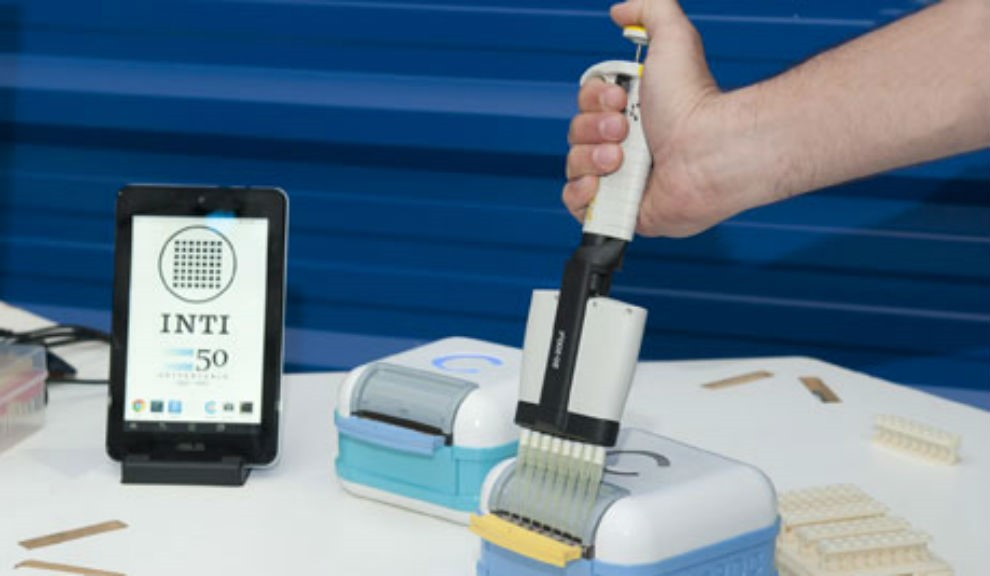
\includegraphics[width=0.5\textwidth]{Figures/Figura_Nano_Poc}
  \caption{NanoPoc platform.}
  \label{fig:Figura_Nano_Poc}
\end{figure}

\section{General Objectives}
The main objective is to generate a biosensor that is easy to manufacture and with high reproducibility. The aim is to improve its use, avoiding the handling of sample preparation between extraction and measurement in the device, for the $``$\textit{in situ}$"$ detection of infectious diseases in humans and animals, depending on the type of bioreceptor developed (Figure ~\ref{fig:Figura_Biosensor_objetivos}).

\begin{figure}[H]
  \centering
    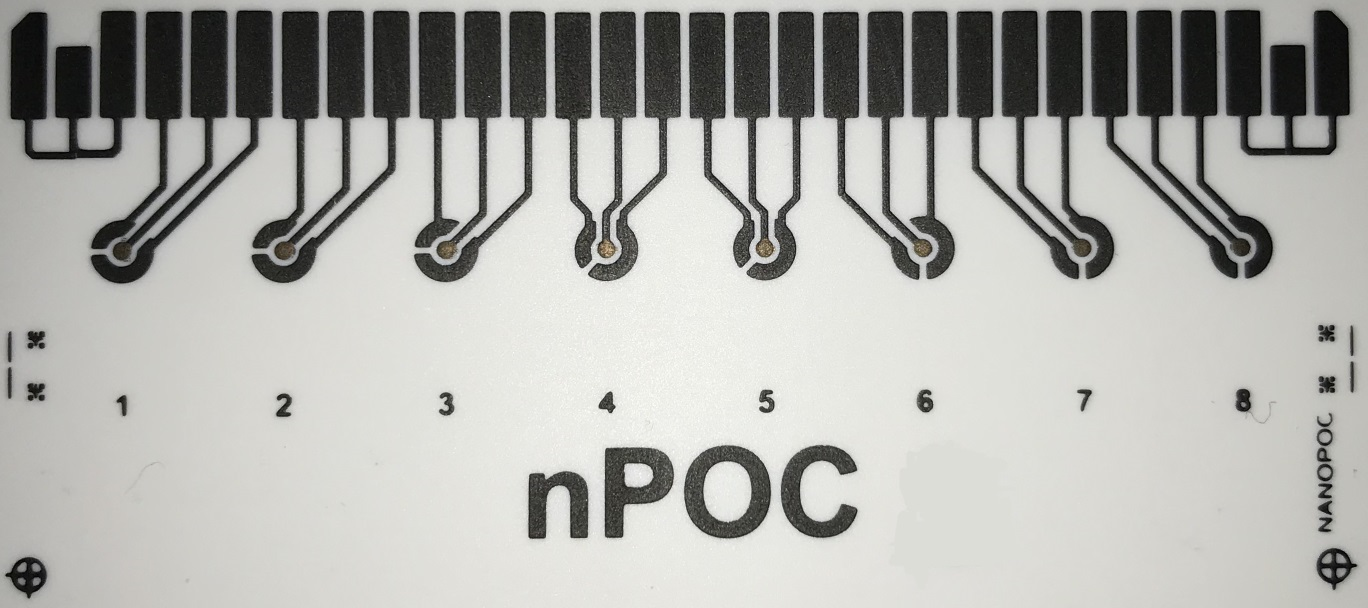
\includegraphics[width=0.5\textwidth]{Figures/Figura_Biosensor_objetivos}
  \caption{Biosensor.}
  \label{fig:Figura_Biosensor_objetivos}
\end{figure}

\section{Specific Objectives}
- Manufacture the sensors with the appropriate form, by means of a controlled deposition of material on the flexible substrate, creating 8 electrochemical cells with the standard dimensions of an 8-channel micropipette (Figure ~\ref{fig:Figura_celda_electroquimica}).\\

\begin{figure}[H]
  \centering
    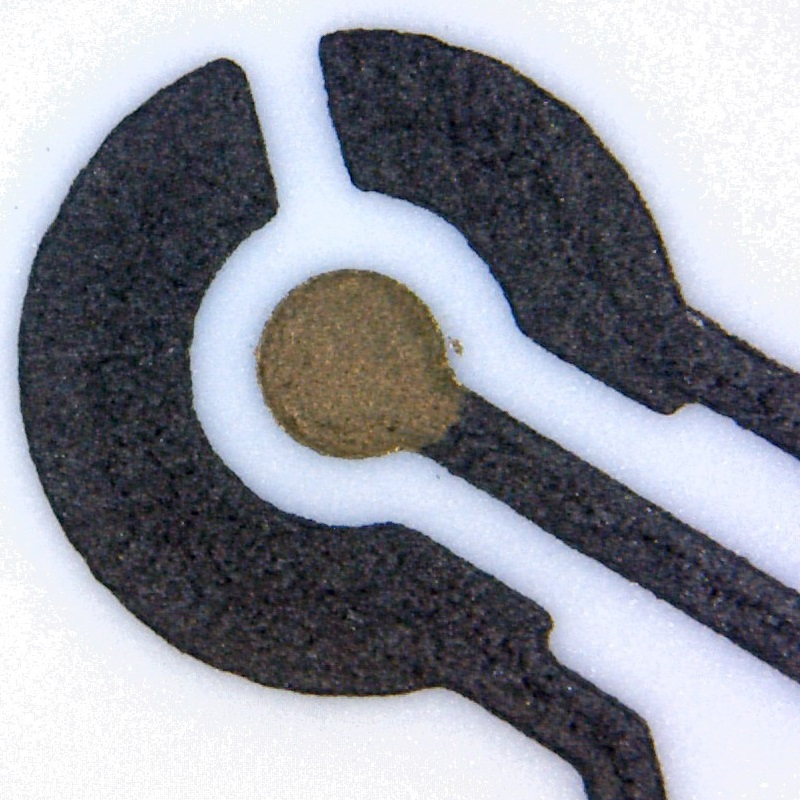
\includegraphics[width=0.35\textwidth]{Figures/Figura_celda_electroquimica}
  \caption{Electrochemical Cell.}
  \label{fig:Figura_celda_electroquimica}
\end{figure}

- Calibrate the inkjet printer in order to obtain the desired biosensor design using a specific ink on the chosen substrate (Figure ~\ref{fig:Figura_impresora_objetivos}).\\

\begin{figure}[H]
  \centering
    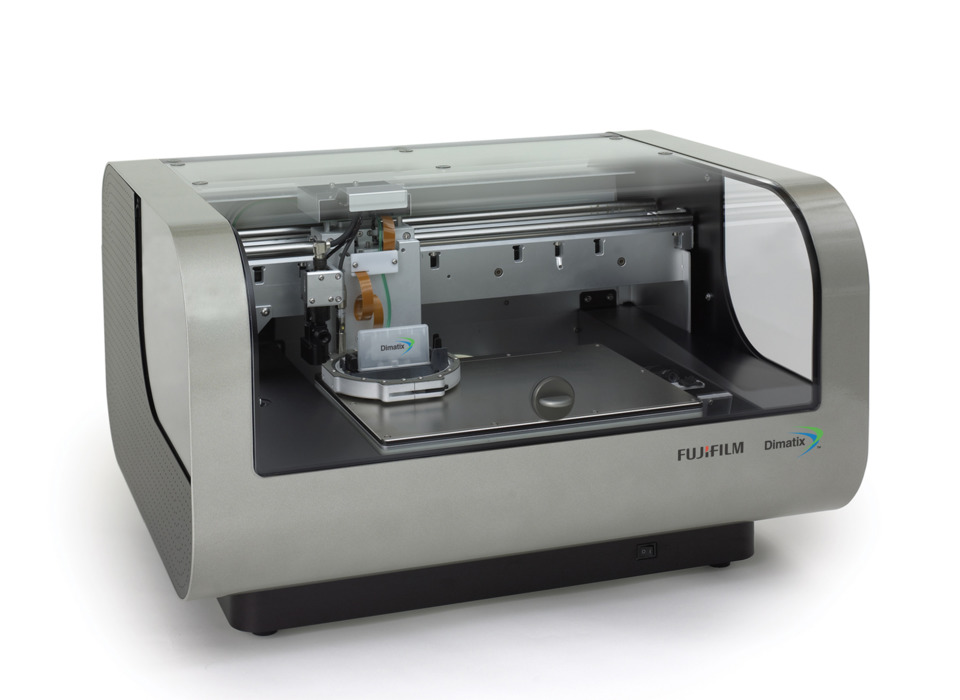
\includegraphics[width=0.5\textwidth]{Figures/Figura_impresora_objetivos}
  \caption{Inkjet Printer.}
  \label{fig:Figura_impresora_objetivos}
\end{figure}

- Obtain a correct response from the biosensors by means of a chemical solution equivalent to a specific analyte using the electrochemical technique of the amperometric type (Figure ~\ref{fig:Figura_caracElectroquim_objetivos}).\\

\begin{figure}[H]
  \centering
    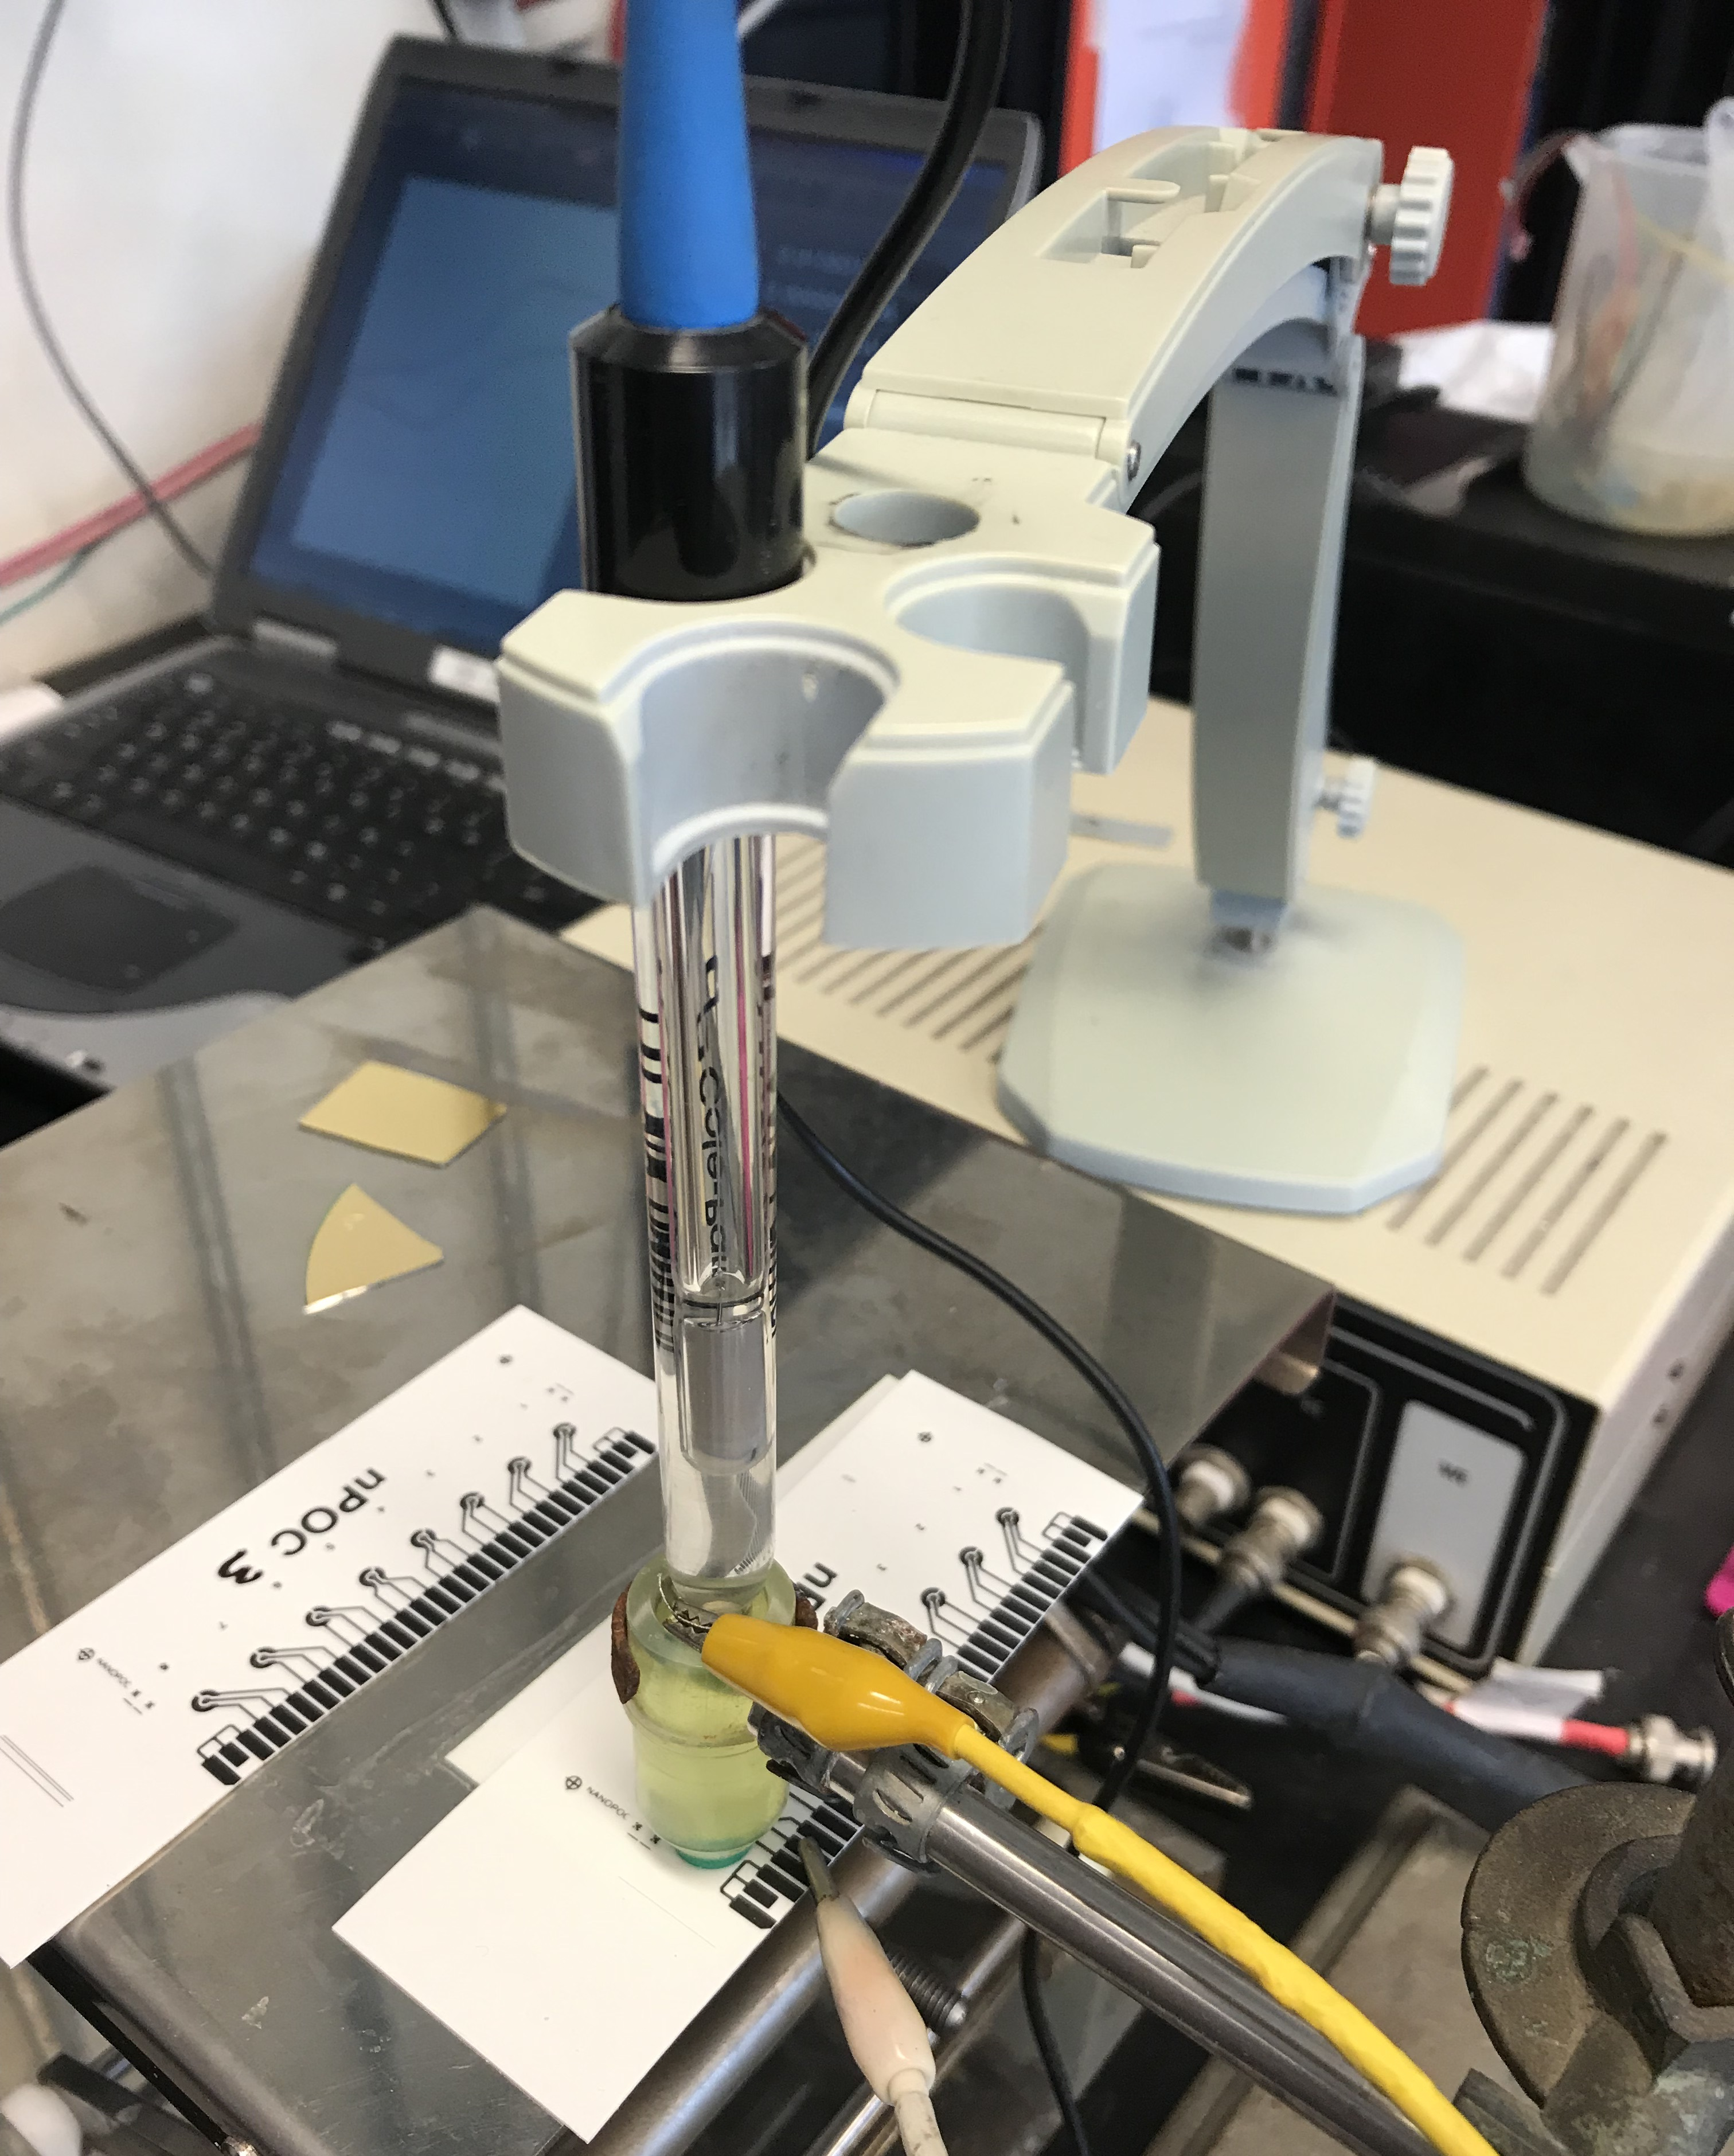
\includegraphics[width=0.4\textwidth]{Figures/Figura_caracElectroquim_objetivos}
  \caption{Electrochemical characterization.}
  \label{fig:Figura_caracElectroquim_objetivos}
\end{figure}
\chapter{Theoretical Framework}
This chapter allows to know the basic concepts required for understanding the development under the proposed project. The field of biosensors is comprised of elementary concepts of electronics, chemistry, materials science, and biology. The functional printed electronics and inkjet printers require theoretical clarifications according to the project to be developed. Fundamental principles of biosensors, functional printed electronics techniques, ink jet printing, the materials to be used and the characterizations to be performed will be analyzed.

\section{Sensors, transducers and biosensors}
A \textbf{sensor} is a device capable of transforming physical or chemical quantities, called instrumentation variables, into electrical quantities through a transducer. These devices can be characterized by different properties such as the measurement range, precision, linearity, repeatability, among others. The instrumentation variables can be magnitudes such as temperature, pressure, humidity, pH, light intensity, distance, acceleration, inclination, displacement, force, torsion, movement, etc. In a broader meaning, it is the expansion of the senses to acquire a knowledge of physical and chemical quantities that, due to their nature or size, cannot be directly perceived by the senses \cite{PallasAreny}.

A \textbf{transducer} transforms the variation in sensor property into an information output detectable by an electronic system. It may or may not have a signal conditioner within the same device, typically with one of the outputs for industrial use: voltage output (V) or standard current output (4 to 20 mA)(Figure ~\ref{fig:Figura_concepto_sensor}).

\begin{figure}[H]
  \centering
    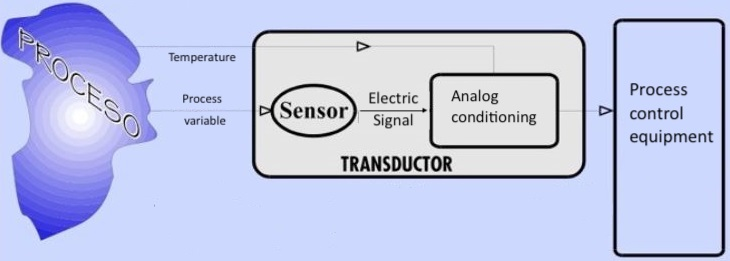
\includegraphics[width=0.8\textwidth]{Figures/Figura_concepto_sensor}
  \caption{Sensor and transducer diagram. Figure taken and traduced from \cite{Hector1}.}
  \label{fig:Figura_concepto_sensor}
\end{figure}

A \textbf{biosensor} can be defined as a device that recognizes a certain analyte by means of a \textbf{bioreceptor} coupled to a \textbf{physicochemical transducer} that converts the biological signal into an electrical signal (Figure ~\ref{fig:Figura_Biosensor}), this signal being proportional to the group of compounds to be determined qualitatively or quantitatively. An analyte is the component of analytical interest of a sample. In the case of biosensors, a protein molecule, a toxin, a peptide, a vitamin or a metal ion are examples. The bioreceptor can be a simple or complex biomolecule (enzymes, antibodies, nucleic acid chains), or based on cells (tissues, organisms) and can be taken from nature or synthesized in a laboratory. The transducer can be of the resonant, optical, thermal, FET (\textit{Field-Effect Transistor}), surface acoustic wave, piezoelectric, or electrochemical type. Within the latter, the conductivity, amperometric, potentiometric and impedometric types can be distinguished \cite{Eggins}.

\begin{figure}[H]
  \centering
    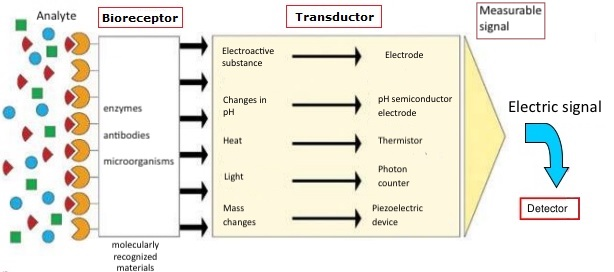
\includegraphics[width=0.8\textwidth]{Figures/Figura_Biosensor}
  \caption{Biosensor diagram: bioreceptor, transducer and electronic signal conditioner. Figure taken and traduced from \cite{Lili1}.}
  \label{fig:Figura_Biosensor}
\end{figure}

Electrochemical transducers are the most widely used in the development of enzyme biosensors. This is because they have a number of advantages, such as:

$\bullet$ Electrochemical measurements can be performed in small volumes, even on the order of nanoliters, with relative ease. This makes such devices especially suitable for monitoring in $``$\textit{in vivo}$"$.

$\bullet$ The electrical signal obtained is the direct transduction of the chemical reaction rate.

$\bullet$ The detection limits that are obtained, normally between 10\textsuperscript{-9} and 10\textsuperscript{-6} mol$\cdot$l\textsuperscript{-1}, are sufficient and adequate for the detection of numerous analytes of interest.

$\bullet$ The relative simplicity and low cost of electrochemical instrumentation allow for easy availability of these devices.

Undoubtedly, in the context of electrochemical biosensors, the most promising in terms of sensitivity, selectivity, size, portability and a minimum volume of sample (analyte) required are the amperometric biosensors, object of study of the present integrating final project. These sensors monitor pharadaic currents (direct transfer of electrons via an oxidation reaction in one electrode and a reduction reaction in the other) between the biological system and a typical electrochemical cell made up of three electrodes: a working electrode \emph{(WE)}, one reference \emph{(RE)} and a counter electrode \emph{(CE)} (Figure ~\ref{fig:Figura_Definicion_Electrodo}). The electrochemical reaction occurs in the \emph{WE}, for which a variable potential is applied with respect to the fixed potential \emph{(RE)} electrode. The current resulting from the chemical reaction circulates between the \emph{WE} and the \emph{CE}. The variation of applied potential and the current measurement are controlled by means of a potentiostat.

\begin{figure}[H]
  \centering
    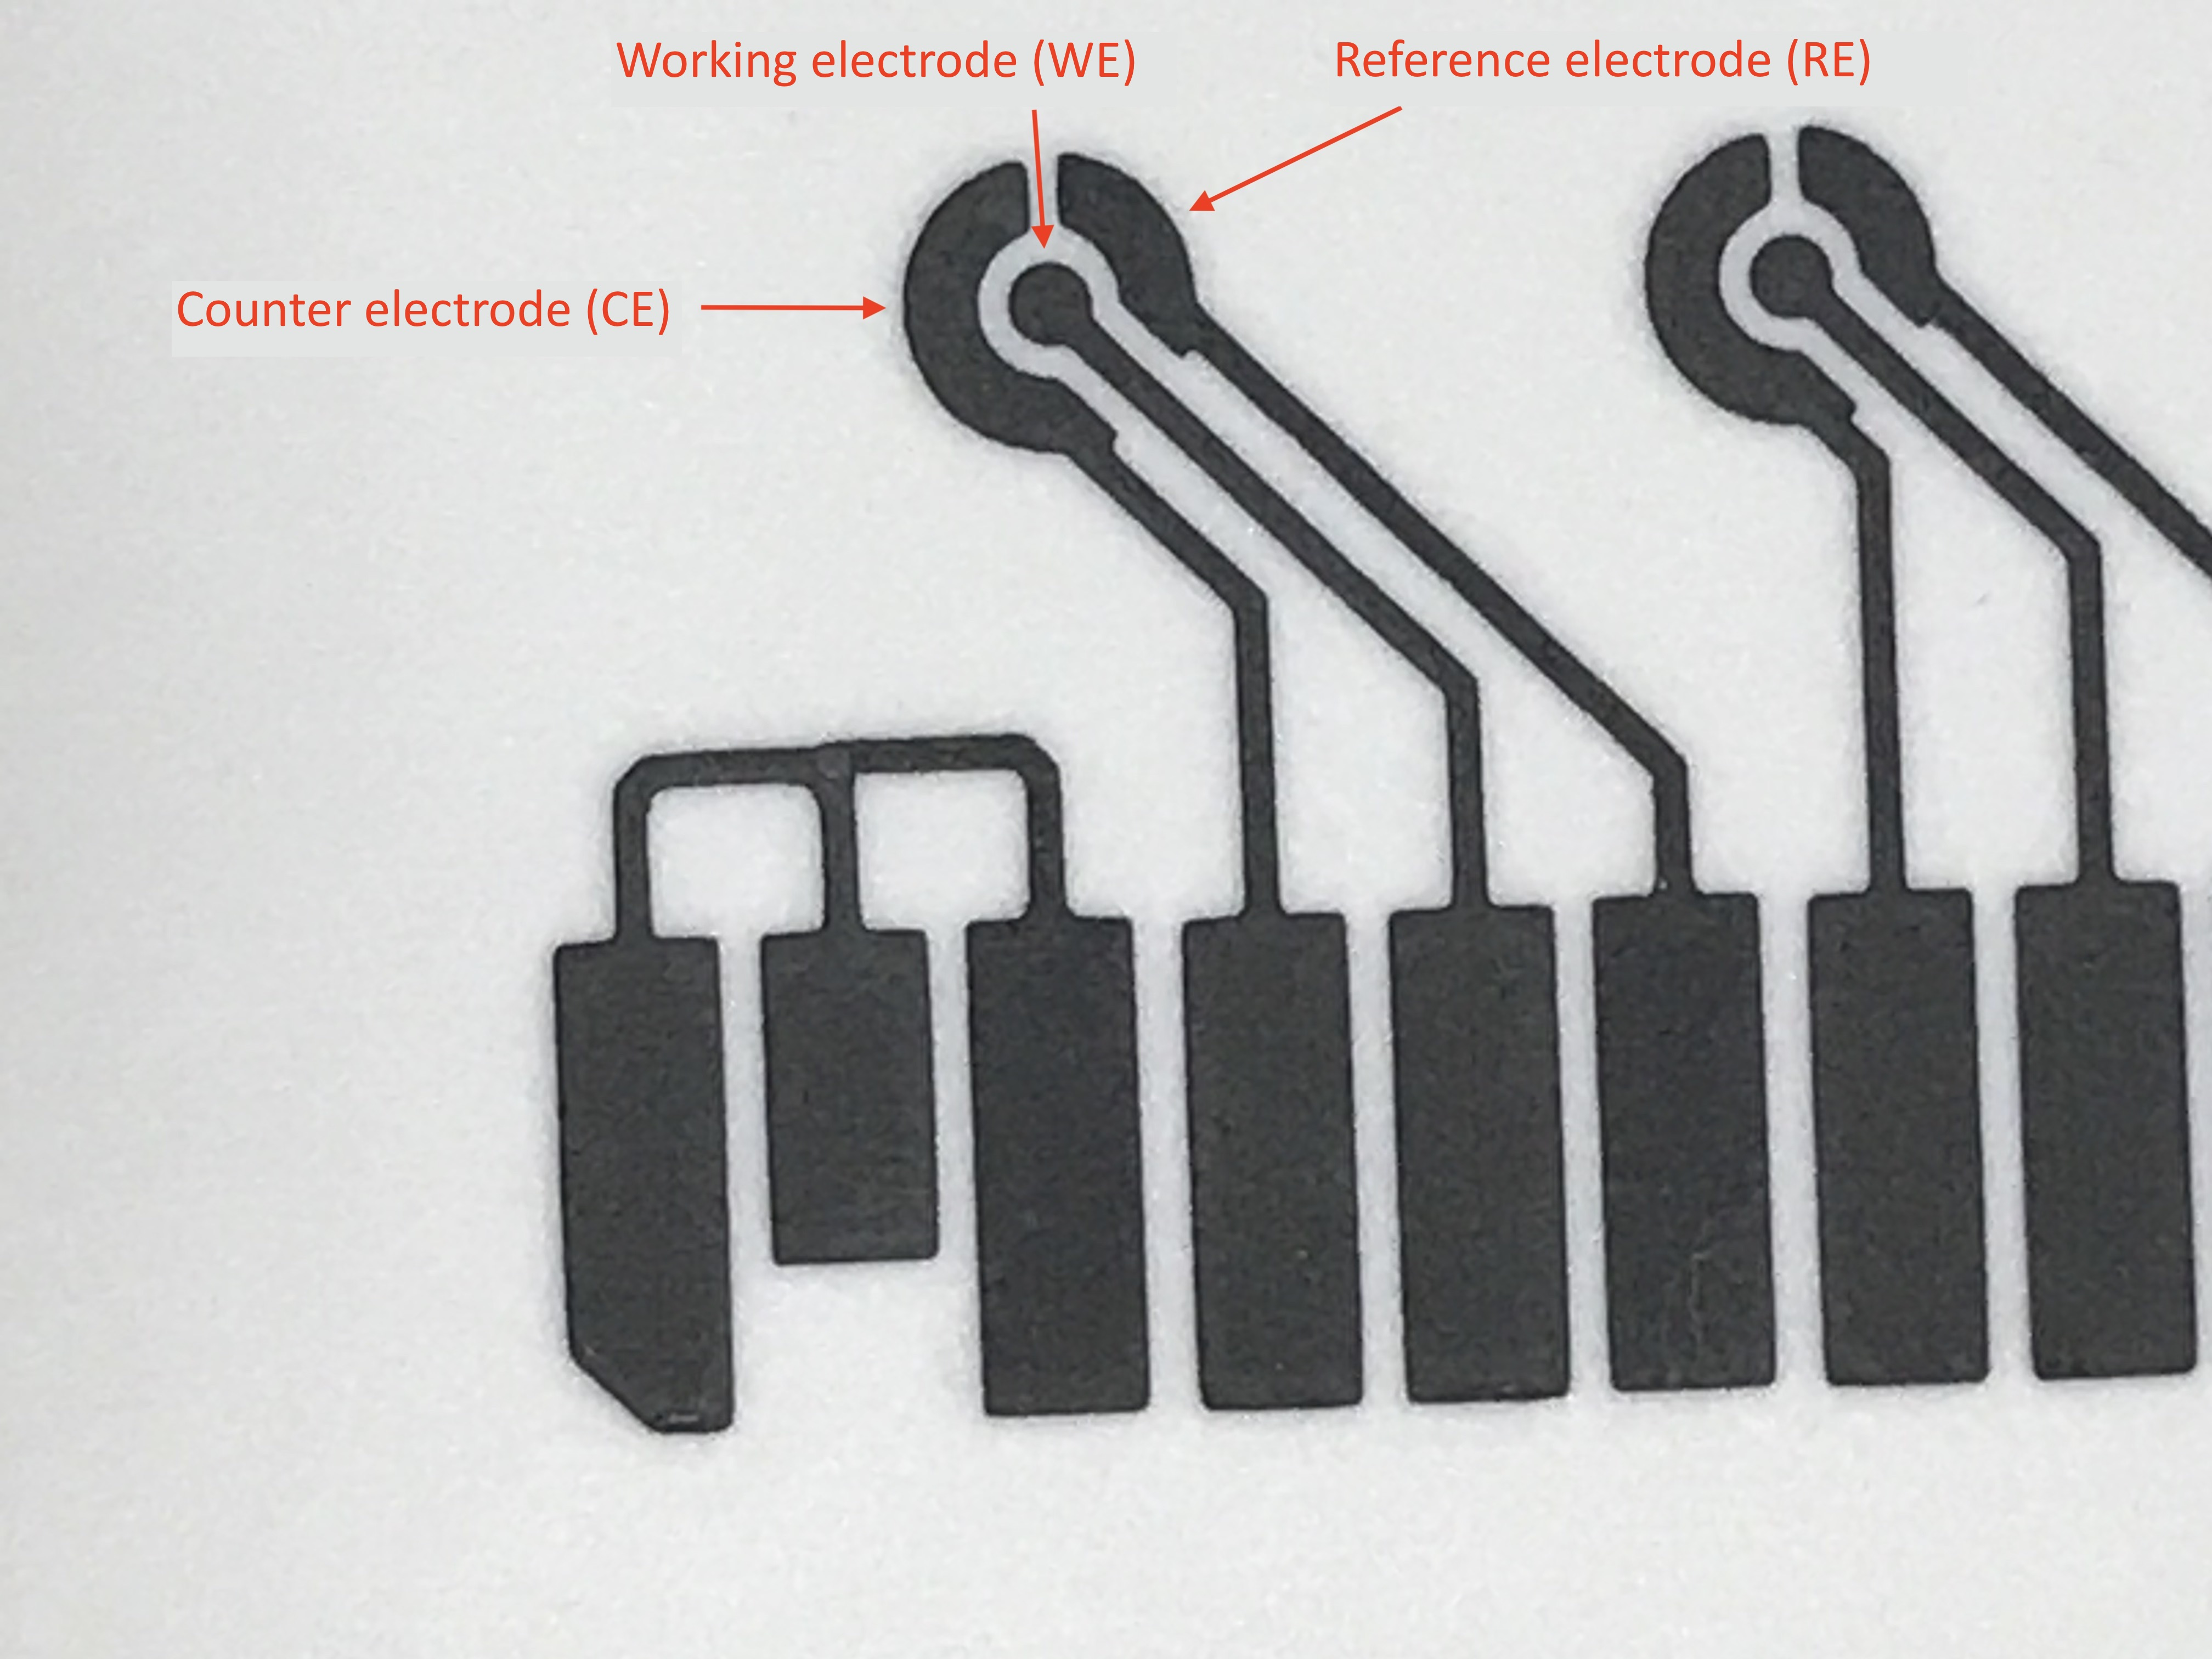
\includegraphics[width=0.5\textwidth]{Figures/Figura_Definicion_Electrodo}
  \caption{Electrochemical Biosensor.}
  \label{fig:Figura_Definicion_Electrodo}
\end{figure}

A potentiostat (Figure ~\ref{fig:Figura_potenciostato}) is an electronic device used to control a three-electrode cell and to perform most electroanalytical experiments. Its function is to apply a variable potential on the \emph{WE} with respect to the fixed potential applied on the \emph{RE} and to measure the resulting current that circulates between the \emph{WE} (where the electrochemical reaction occurs) and the \emph{CE}.

\begin{figure}[H]
  \centering
    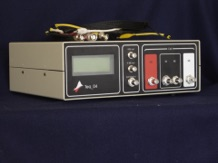
\includegraphics[width=0.5\textwidth]{Figures/Figura_potenciostato}
  \caption{Potentiostat used for electrochemical characterization.}
  \label{fig:Figura_potenciostato}
\end{figure}

\section{Functional Printed Electronics}
Taking advantage of technological advances in micro and nano electronics, it was decided to implement the biosensors using printing techniques, seeking in this way to have disposable sensor arrays, of simple manufacturing and high production scale. The biosensors can be printed on ceramic (Al\textsubscript{2}O\textsubscript{3}), acrylic or PMMA (Methyl Methacrylate Polymer) substrates, or on flexible material like PET (Polyethylene Terephthalate), Valox, etc., using different techniques, such as Screen Printing or Inkjet printing.

Silk-screen printing, typical of thick film technology, allows the manufacture of electronic circuits and sensors that are obtained by depositing layers of inks (typically resistive, conductive and dielectric), by means of a rubber spatula that moves transversely through a mesh or mask, with a given pattern, on an isolated substrate, usually ceramic. The spatula forces the ink to pass through the openings of the stainless steel mesh. They are subsequently sintered at peak temperatures of 850ºC to remove the solvents from the inks, fix the electrical characteristics of the inks and adhere the layers to the substrate (Figure ~\ref{fig:Figura_serigrafia}).

\begin{figure}[H]
  \centering
    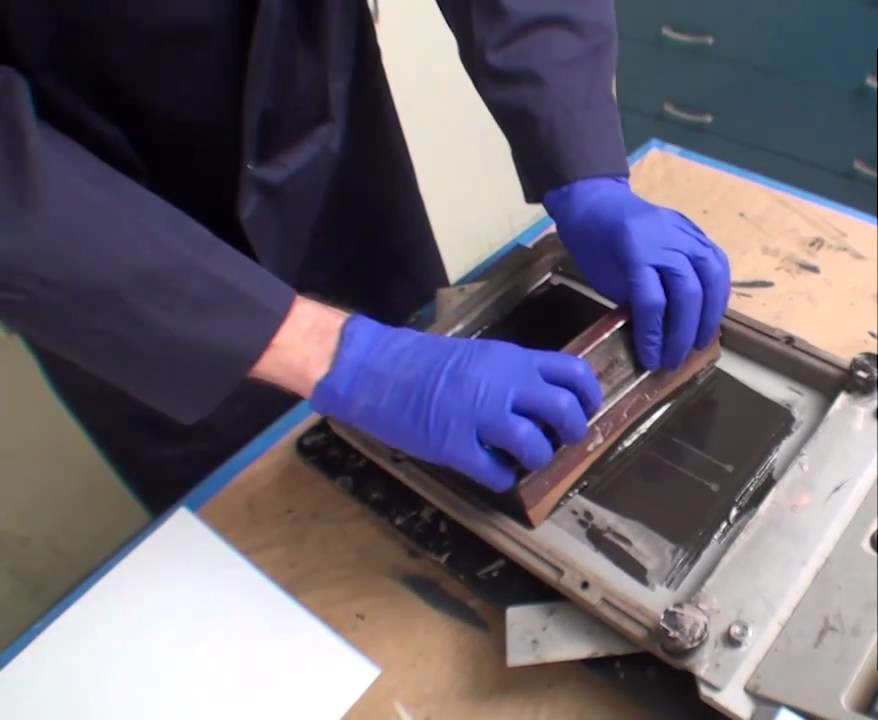
\includegraphics[width=0.5\textwidth]{Figures/Figura_serigrafia}
  \caption{Manual Silk-screen printing.}
  \label{fig:Figura_serigrafia}
\end{figure}

Inkjet printing uses piezoelectric heads to deposit ink droplets according to software controlled coordinates. The inks can be conductive, semiconductive, or dielectric (Figure ~\ref{fig:Figura_inkjet_dimatix}).

\begin{figure}[H]
  \centering
    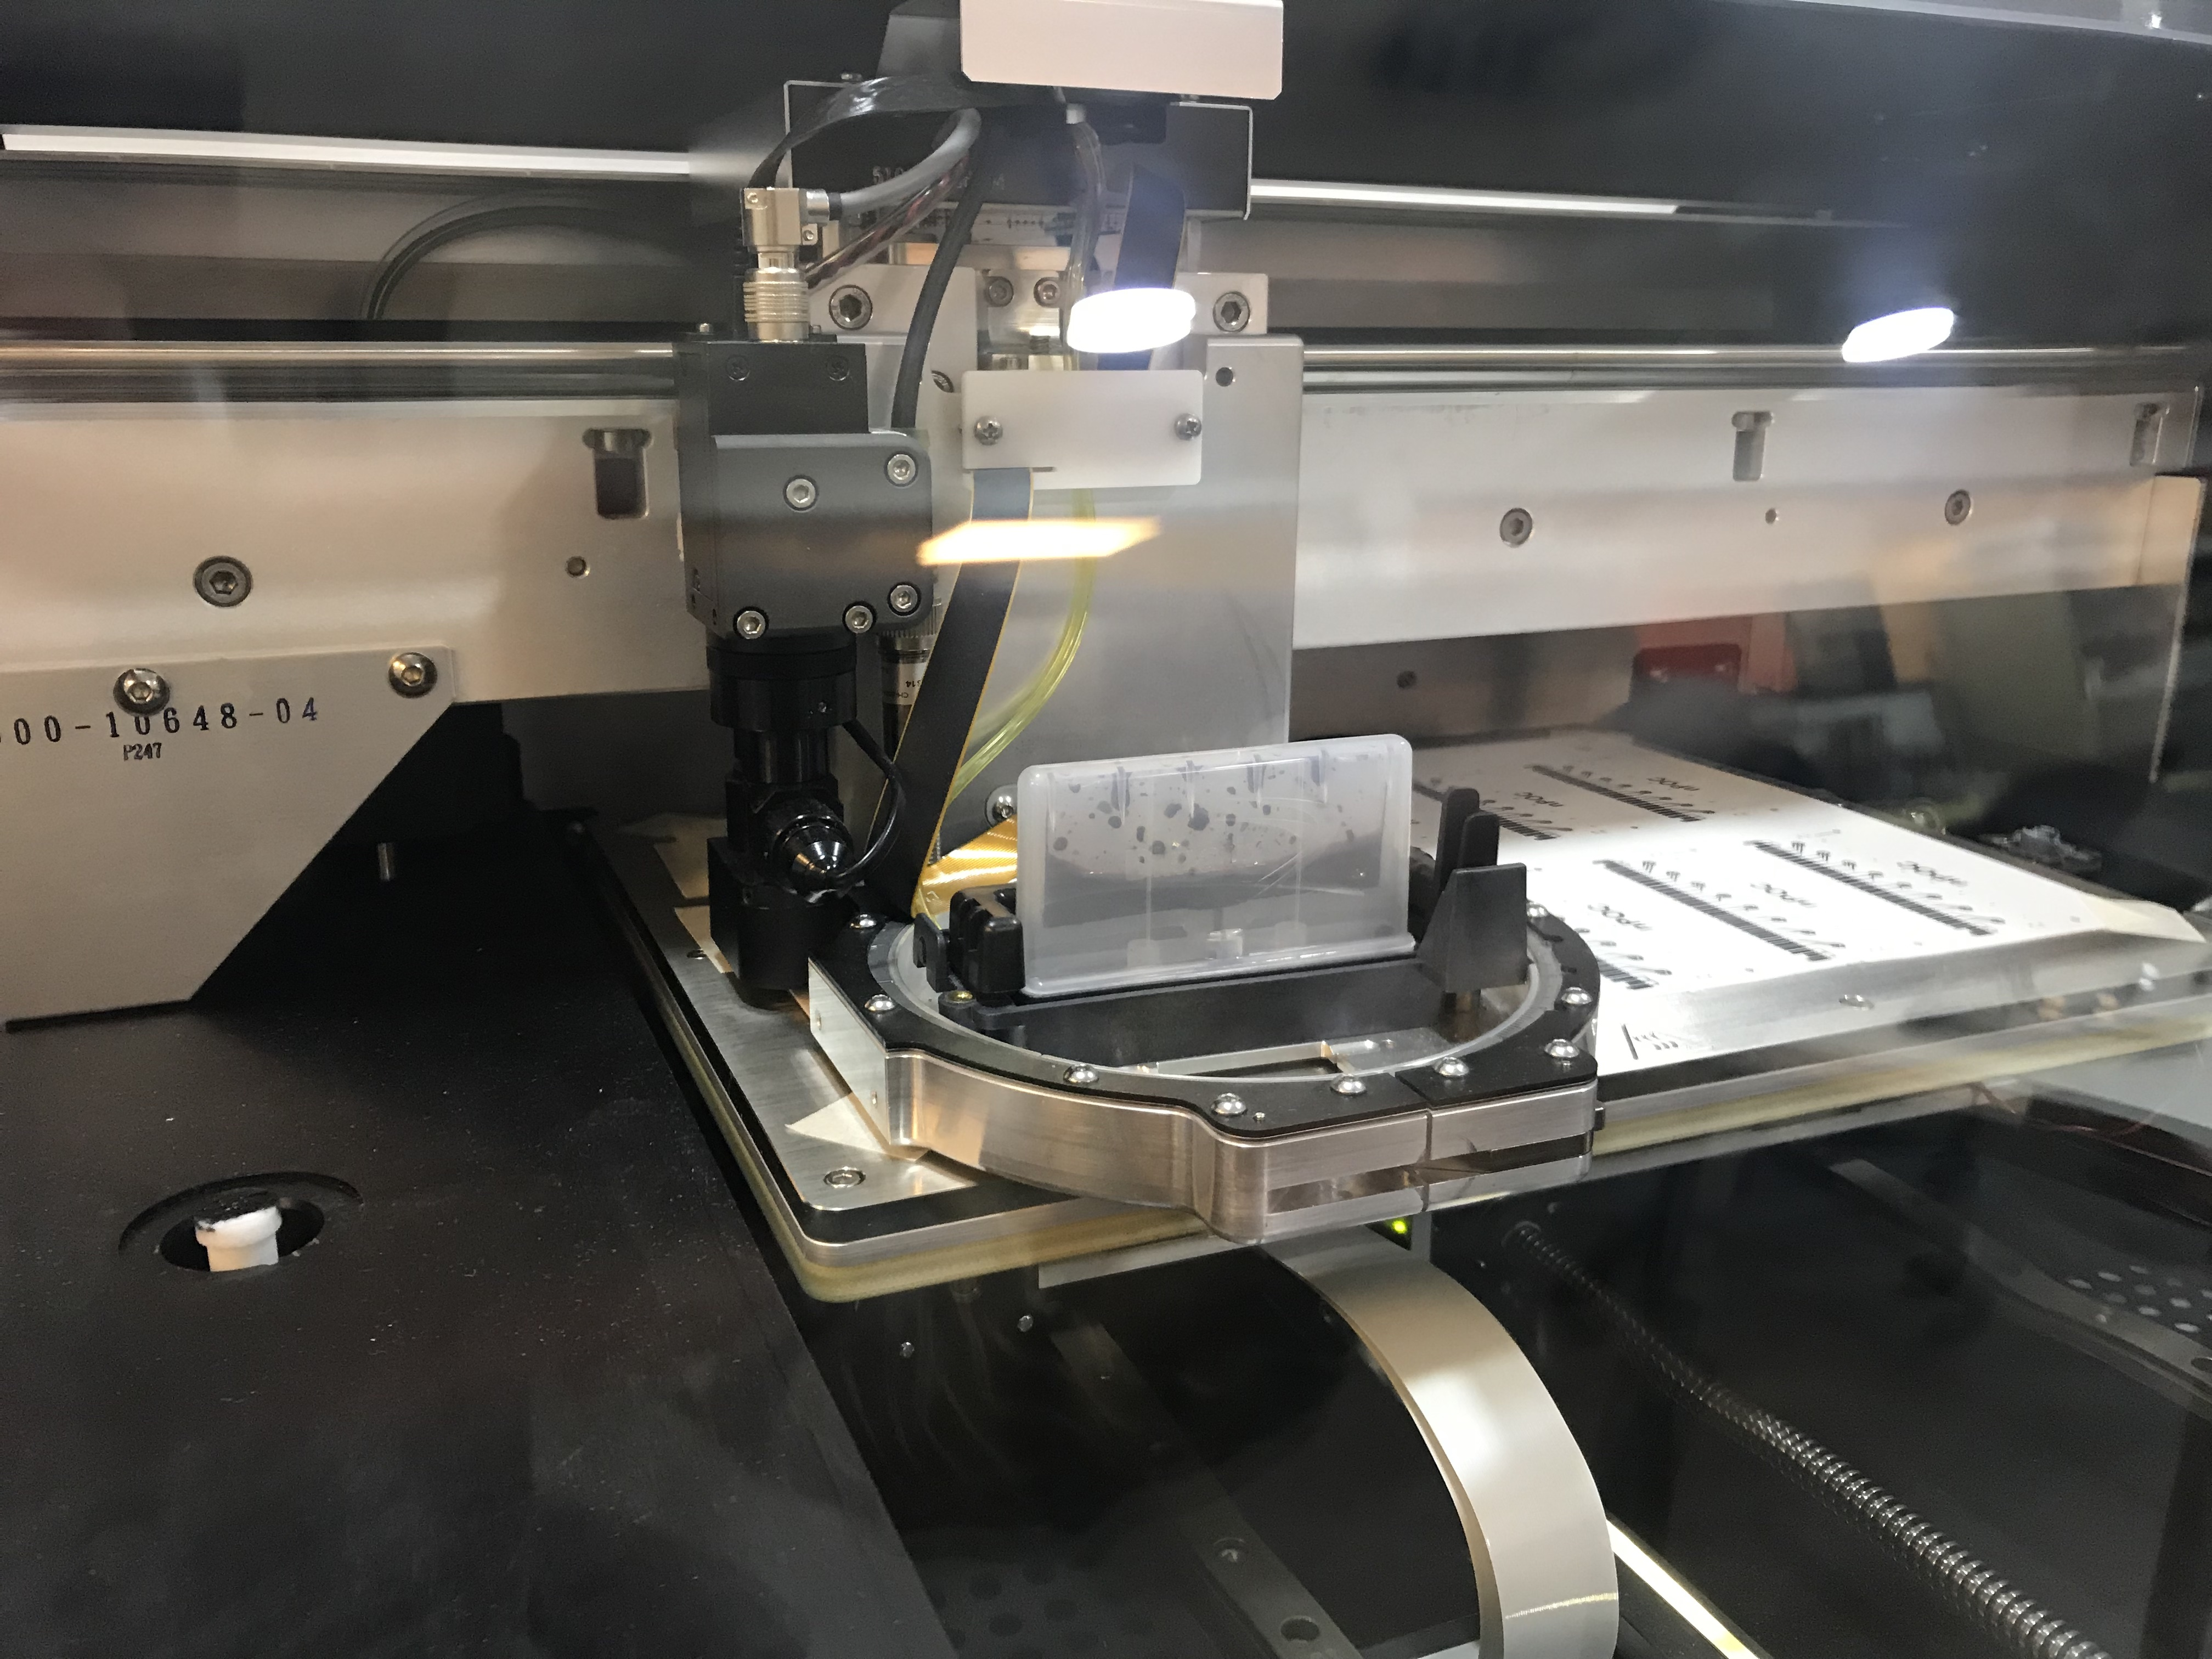
\includegraphics[width=0.5\textwidth]{Figures/Figura_inkjet_dimatix}
  \caption{Inkjet printing.}
  \label{fig:Figura_inkjet_dimatix}
\end{figure}

In this thesis, an electrochemical biosensor on flexible substrate is implemented using an Inkjet printer and the amperometric method is used to characterize it. The versatility, ease of use and innovative type of manufacturing are some of the most notable reasons why it was decided to carry out the present project in an inkjet printer.

\subsection{Inkjet printer}
As mentioned, the Inkjet type printer uses a piezoelectric head for ink deposition  (Figure ~\ref{fig:Figura_Piezoelectrico}). This head contains a reservoir with a crystal that, when a potential is applied, it moves generating a mechanical force in the tank, which causes the ejection of a drop of ink.

\begin{figure}[H]
  \centering
    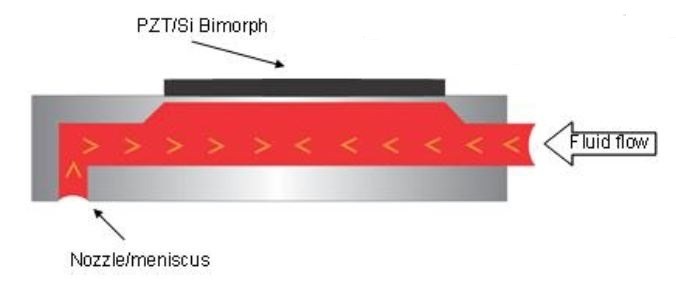
\includegraphics[width=0.5\textwidth]{Figures/Figura_Piezoelectrico}
  \caption{Piezoelectric head diagram.}
  \label{fig:Figura_Piezoelectrico}
\end{figure}

For this, a waveform specified by the manufacturer must be applied (Figure ~\ref{fig:Figura_Waveform_Dimatix}), although it must be modified for each type of ink.

\begin{figure}[H]
  \centering
    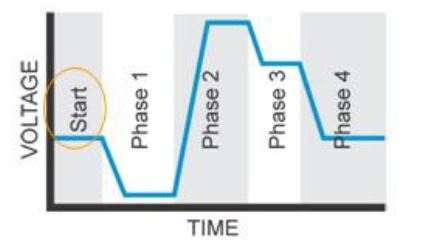
\includegraphics[width=0.5\textwidth]{Figures/Figura_Waveform_Dimatix}
  \caption{Waveform specified for piezoelectric print head.}
  \label{fig:Figura_Waveform_Dimatix}
\end{figure}

In the stage called $``$Start$"$ or also identified as $``$Standby$"$, the piezoelectric is slightly deflected generating an ink meniscus, preventing the involuntary ink drop. In $``$phase 1$"$ the electric potential is decreased and the piezoelectric moves upwards, allowing the reservoir to fill. In $``$phase 2$"$ the voltage increases, initiating the formation of the drop. Once the drop is formed, in $``$phase 3$"$ the voltage decreases again, releasing the drop from the head. $``$Phase 4$"$ is the return to the $``$Start$"$ electric potential (Figure ~\ref{fig:Figura_etapas_eyector}).

\begin{figure}[H]
  \centering
    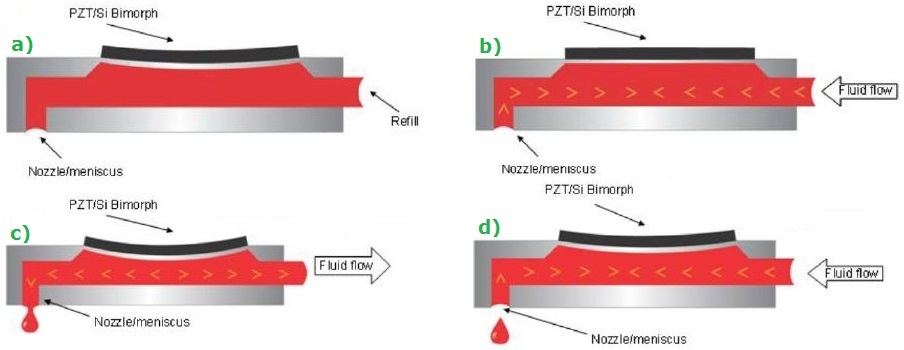
\includegraphics[width=0.8\textwidth]{Figures/Figura_etapas_eyector}
  \caption{a) Start/Standby Stage, b) Phase 1, c) Phase 2, d) Phase 3 and back to Standby.}
  \label{fig:Figura_etapas_eyector}
\end{figure}

The modifiable parameters of this waveform are the voltage level (percentage relative to the voltage set to the ejector), the slew rate that specifies the slope of the ramps between phases and the duration of each segment \cite{DimatixUM}.

The head, responsible for ejecting the ink, is a piece of \textit{MEMS} type (Micro-Electro-Mechanical Systems). Because of this, they are about the size of a thermal inkjet printer, but superior in technology (Figure ~\ref{fig:Figura_cabezal}).

\begin{figure}[H]
  \centering
    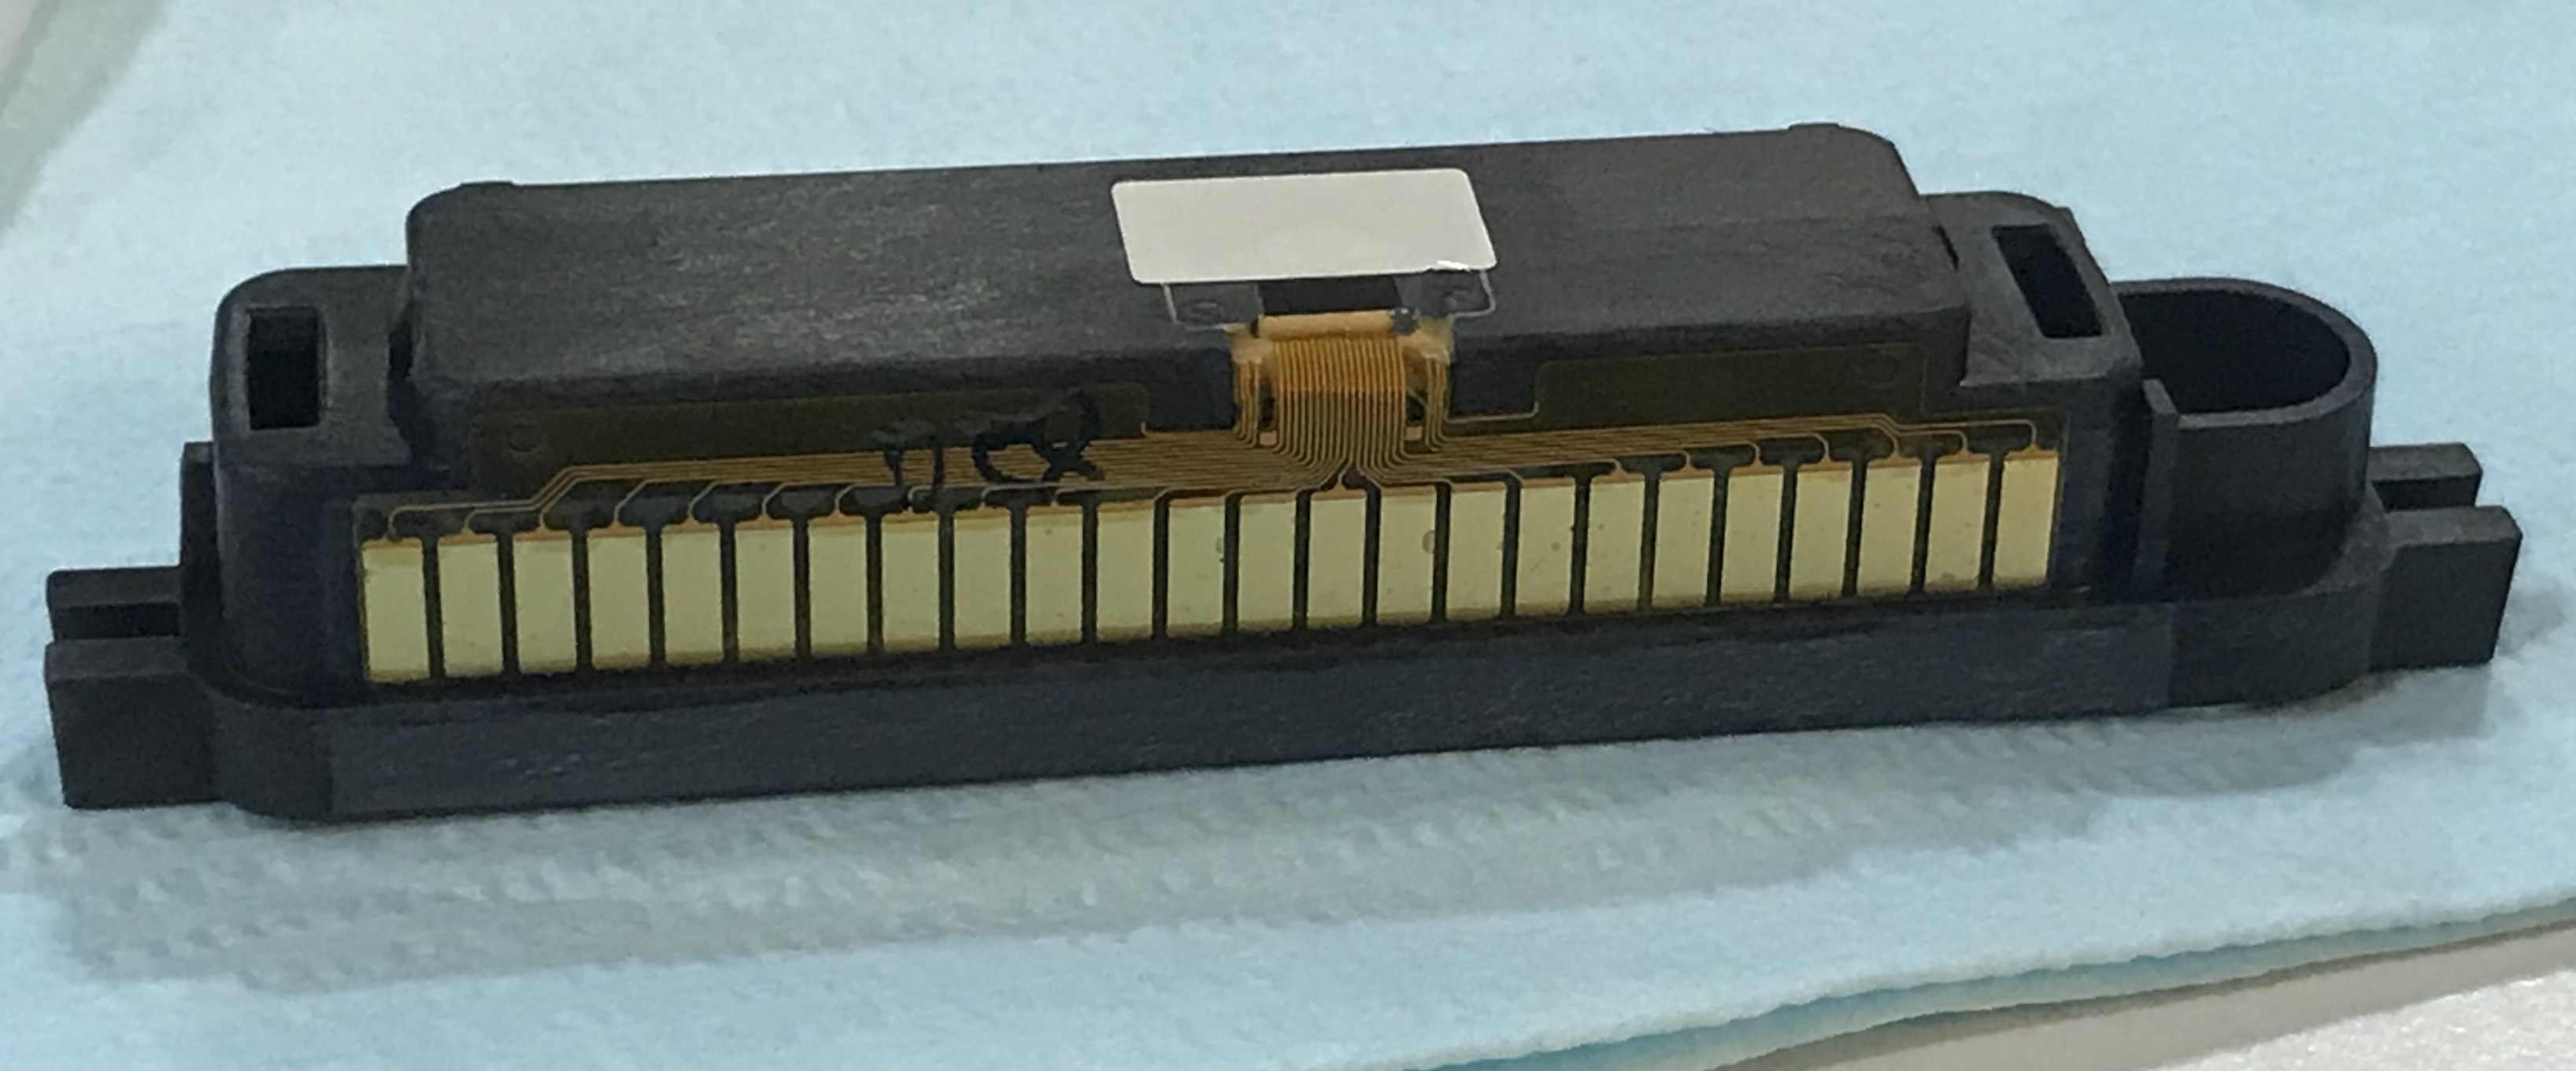
\includegraphics[width=0.5\textwidth]{Figures/Figura_cabezal}
  \caption{Fujifilm Dimatix DMP-2850 Printer Head.}
  \label{fig:Figura_cabezal}
\end{figure}

The one corresponding to the Fujifilm Dimatix DMP2850 printer has 16 ejectors, with which different combinations can be made, achieving different spacing between drops and therefore, different line widths. The complete cartridge consists of the head and a 3 ml reservoir, which can be filled with inks of different materials (Figure ~\ref{fig:Figura_cartucho_completo}).

\begin{figure}[H]
  \centering
    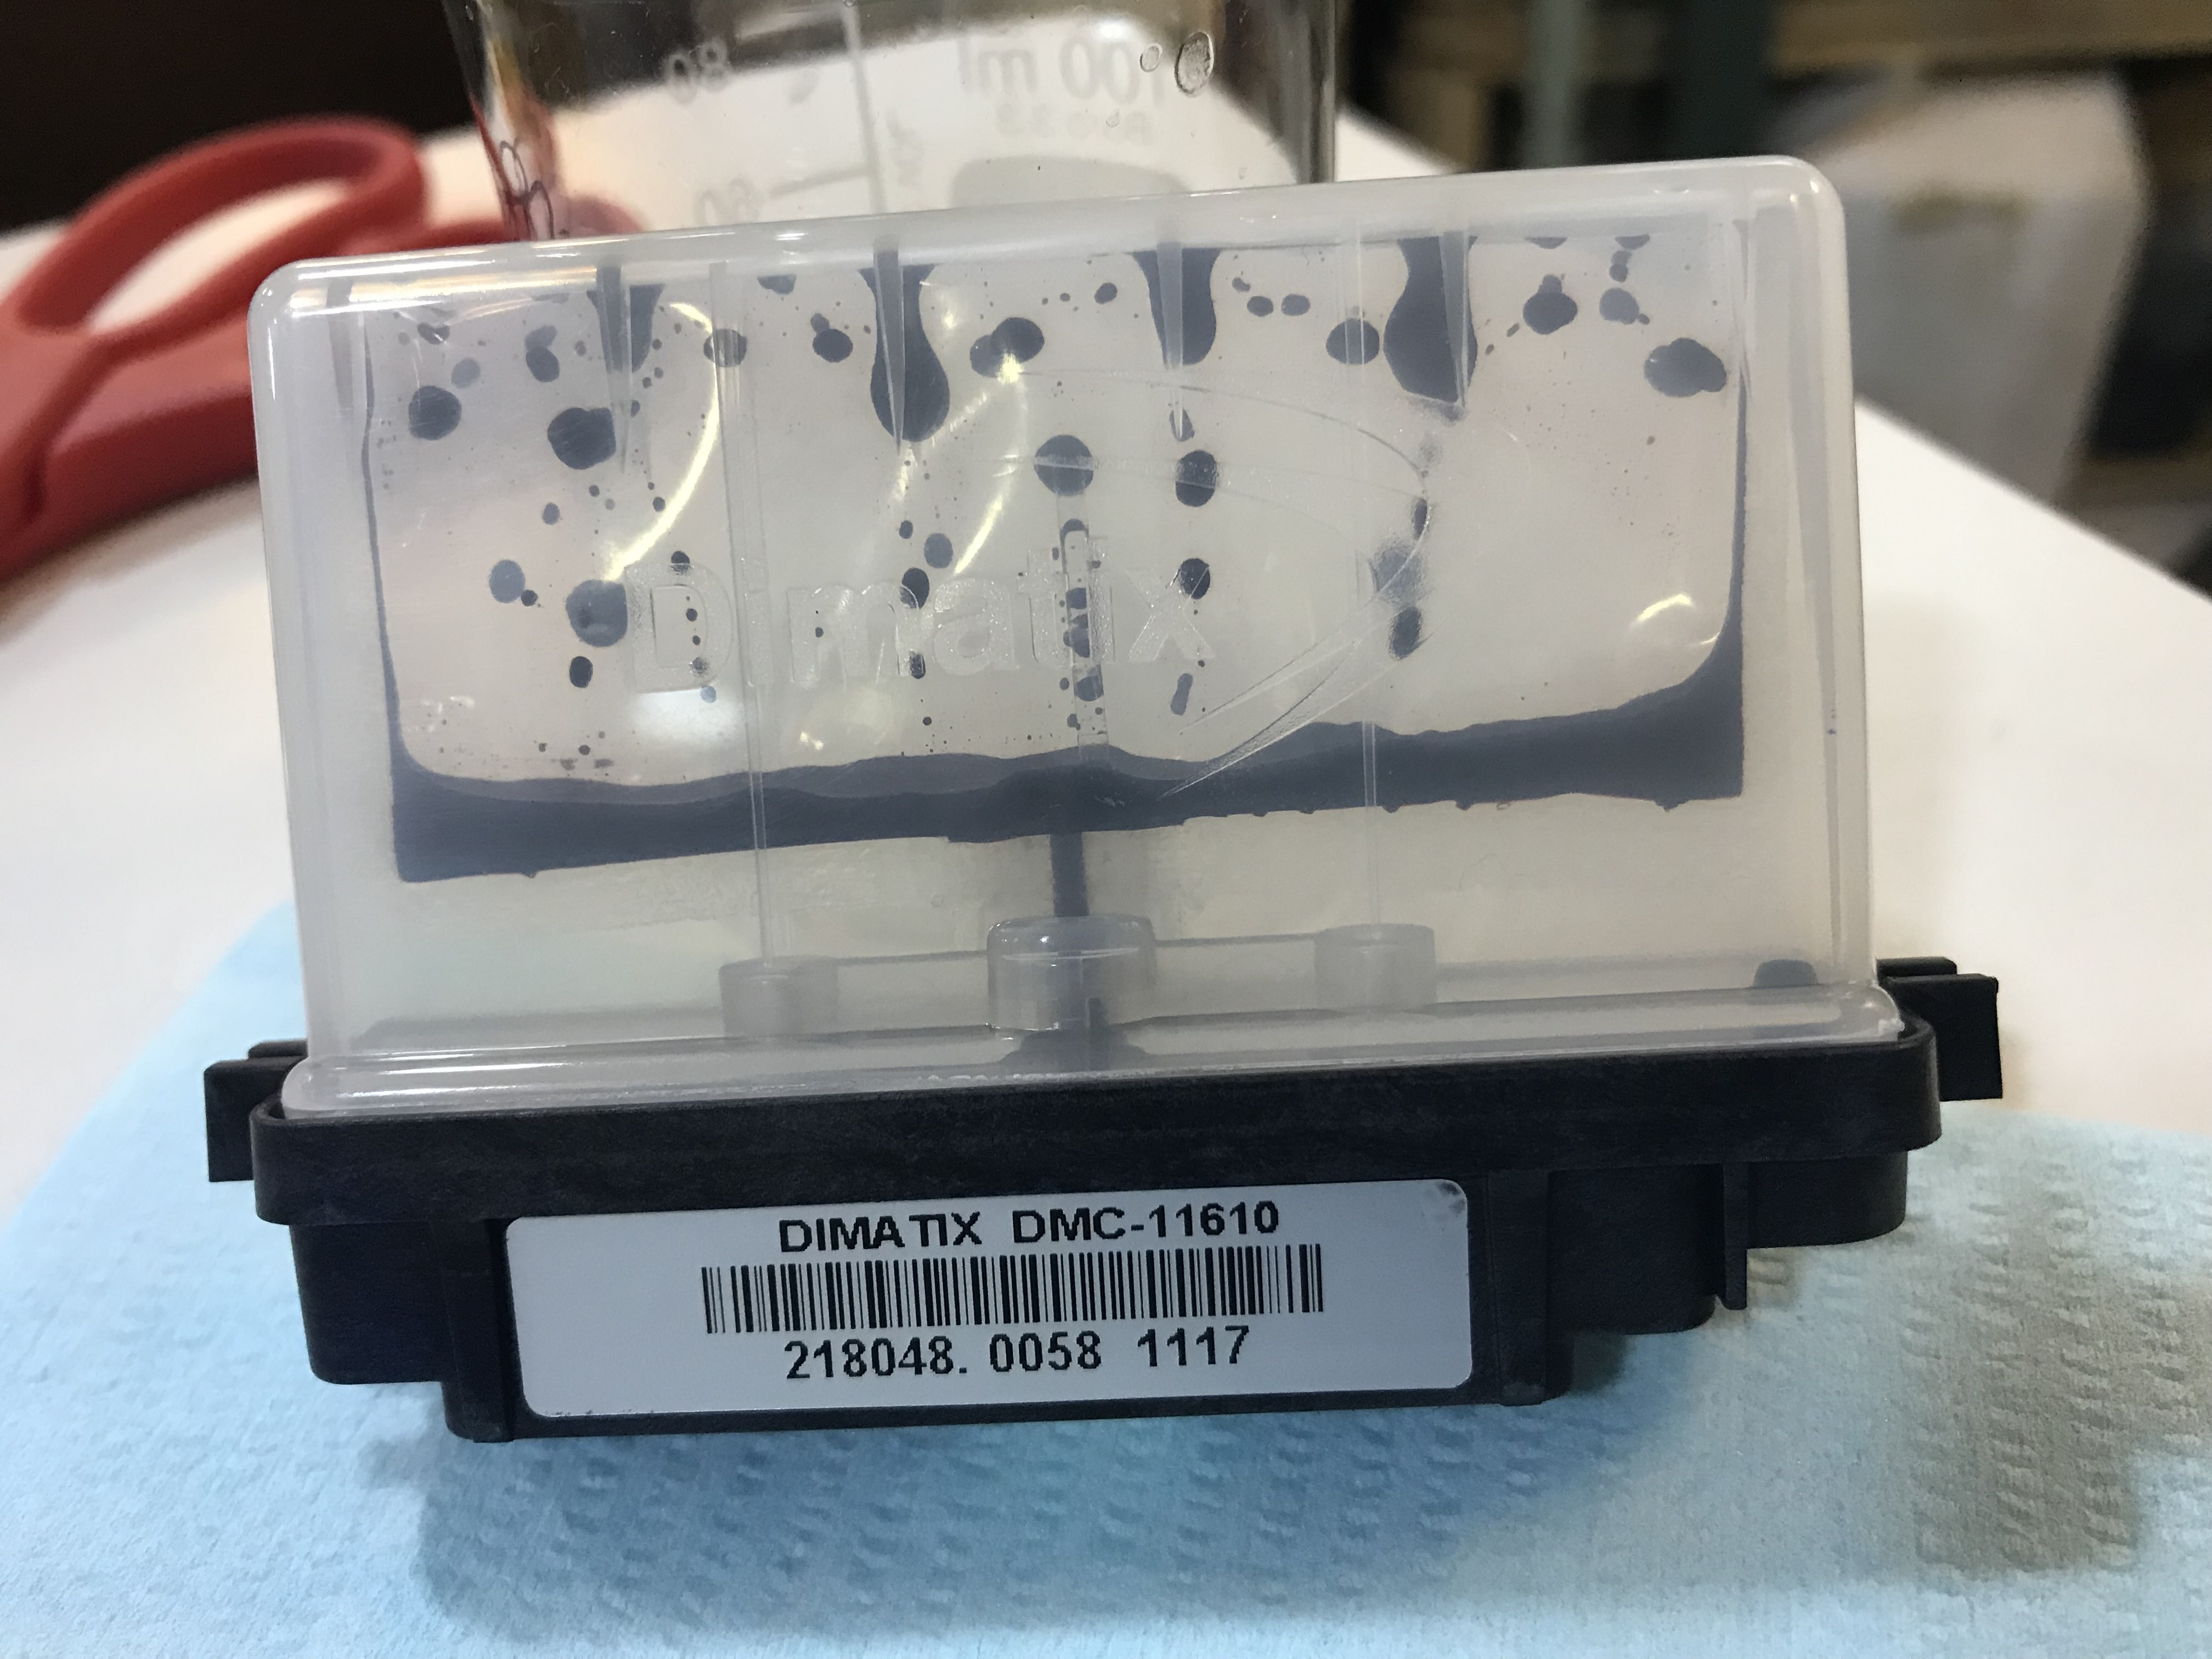
\includegraphics[width=0.5\textwidth]{Figures/Figura_cartucho_completo}
  \caption{Fujifilm Dimatix DMP-2850 Printer Cartridge.}
  \label{fig:Figura_cartucho_completo}
\end{figure}

As examples, Fujifilm reports that graphics, electronics, displays, chemicals, optical objects, photovoltaic objects, 3D mechanical objects, and life science elements such as DNA strands can be printed.

\subsection{Gold nanoparticles ink}
An ink with gold nanoparticles, manufactured by \textit{C-INK} Company under the trade name \textit{Drycure Au-JB 1010B}, will be used in this project  \cite{DrycureAu}. This ink contains nanometric particles of gold (Au). Although the effect of these on the human body has not been proven, extreme caution should be exercised when handling it. For this reason, the manufacturer recommends using it in a good ventilated environment or with an extraction system, using respiratory protection in case of evaporation. Gloves, glasses and work clothes should be worn at all times, especially when handling the ink.

Within its composition there is, given as a percentage in weight, 9-11 \% of Gold, 36-40 \% of water, 48-52 \% of Glycerol, 0.1-1.0 \% of Alcohol, 0.1-0.5 \% of \textit{Acetylene glycol} and 0.1-2.0 \% of Polyester resin.

As physical and chemical characteristics, it is indicated that the ink is liquid, it is a miscible solution, it has a density of 1.10 to 1.20 g/ml and a viscosity of 9 to 11 mPa$\cdot$s.

Since the ink is formulated based on water, it must be kept at low temperatures and hermetically sealed to avoid solvent evaporation or excessive humidity, which can cause alterations in its characteristics (Figure ~\ref{fig:Figura_tinta_Au}).

\begin{figure}[H]
  \centering
    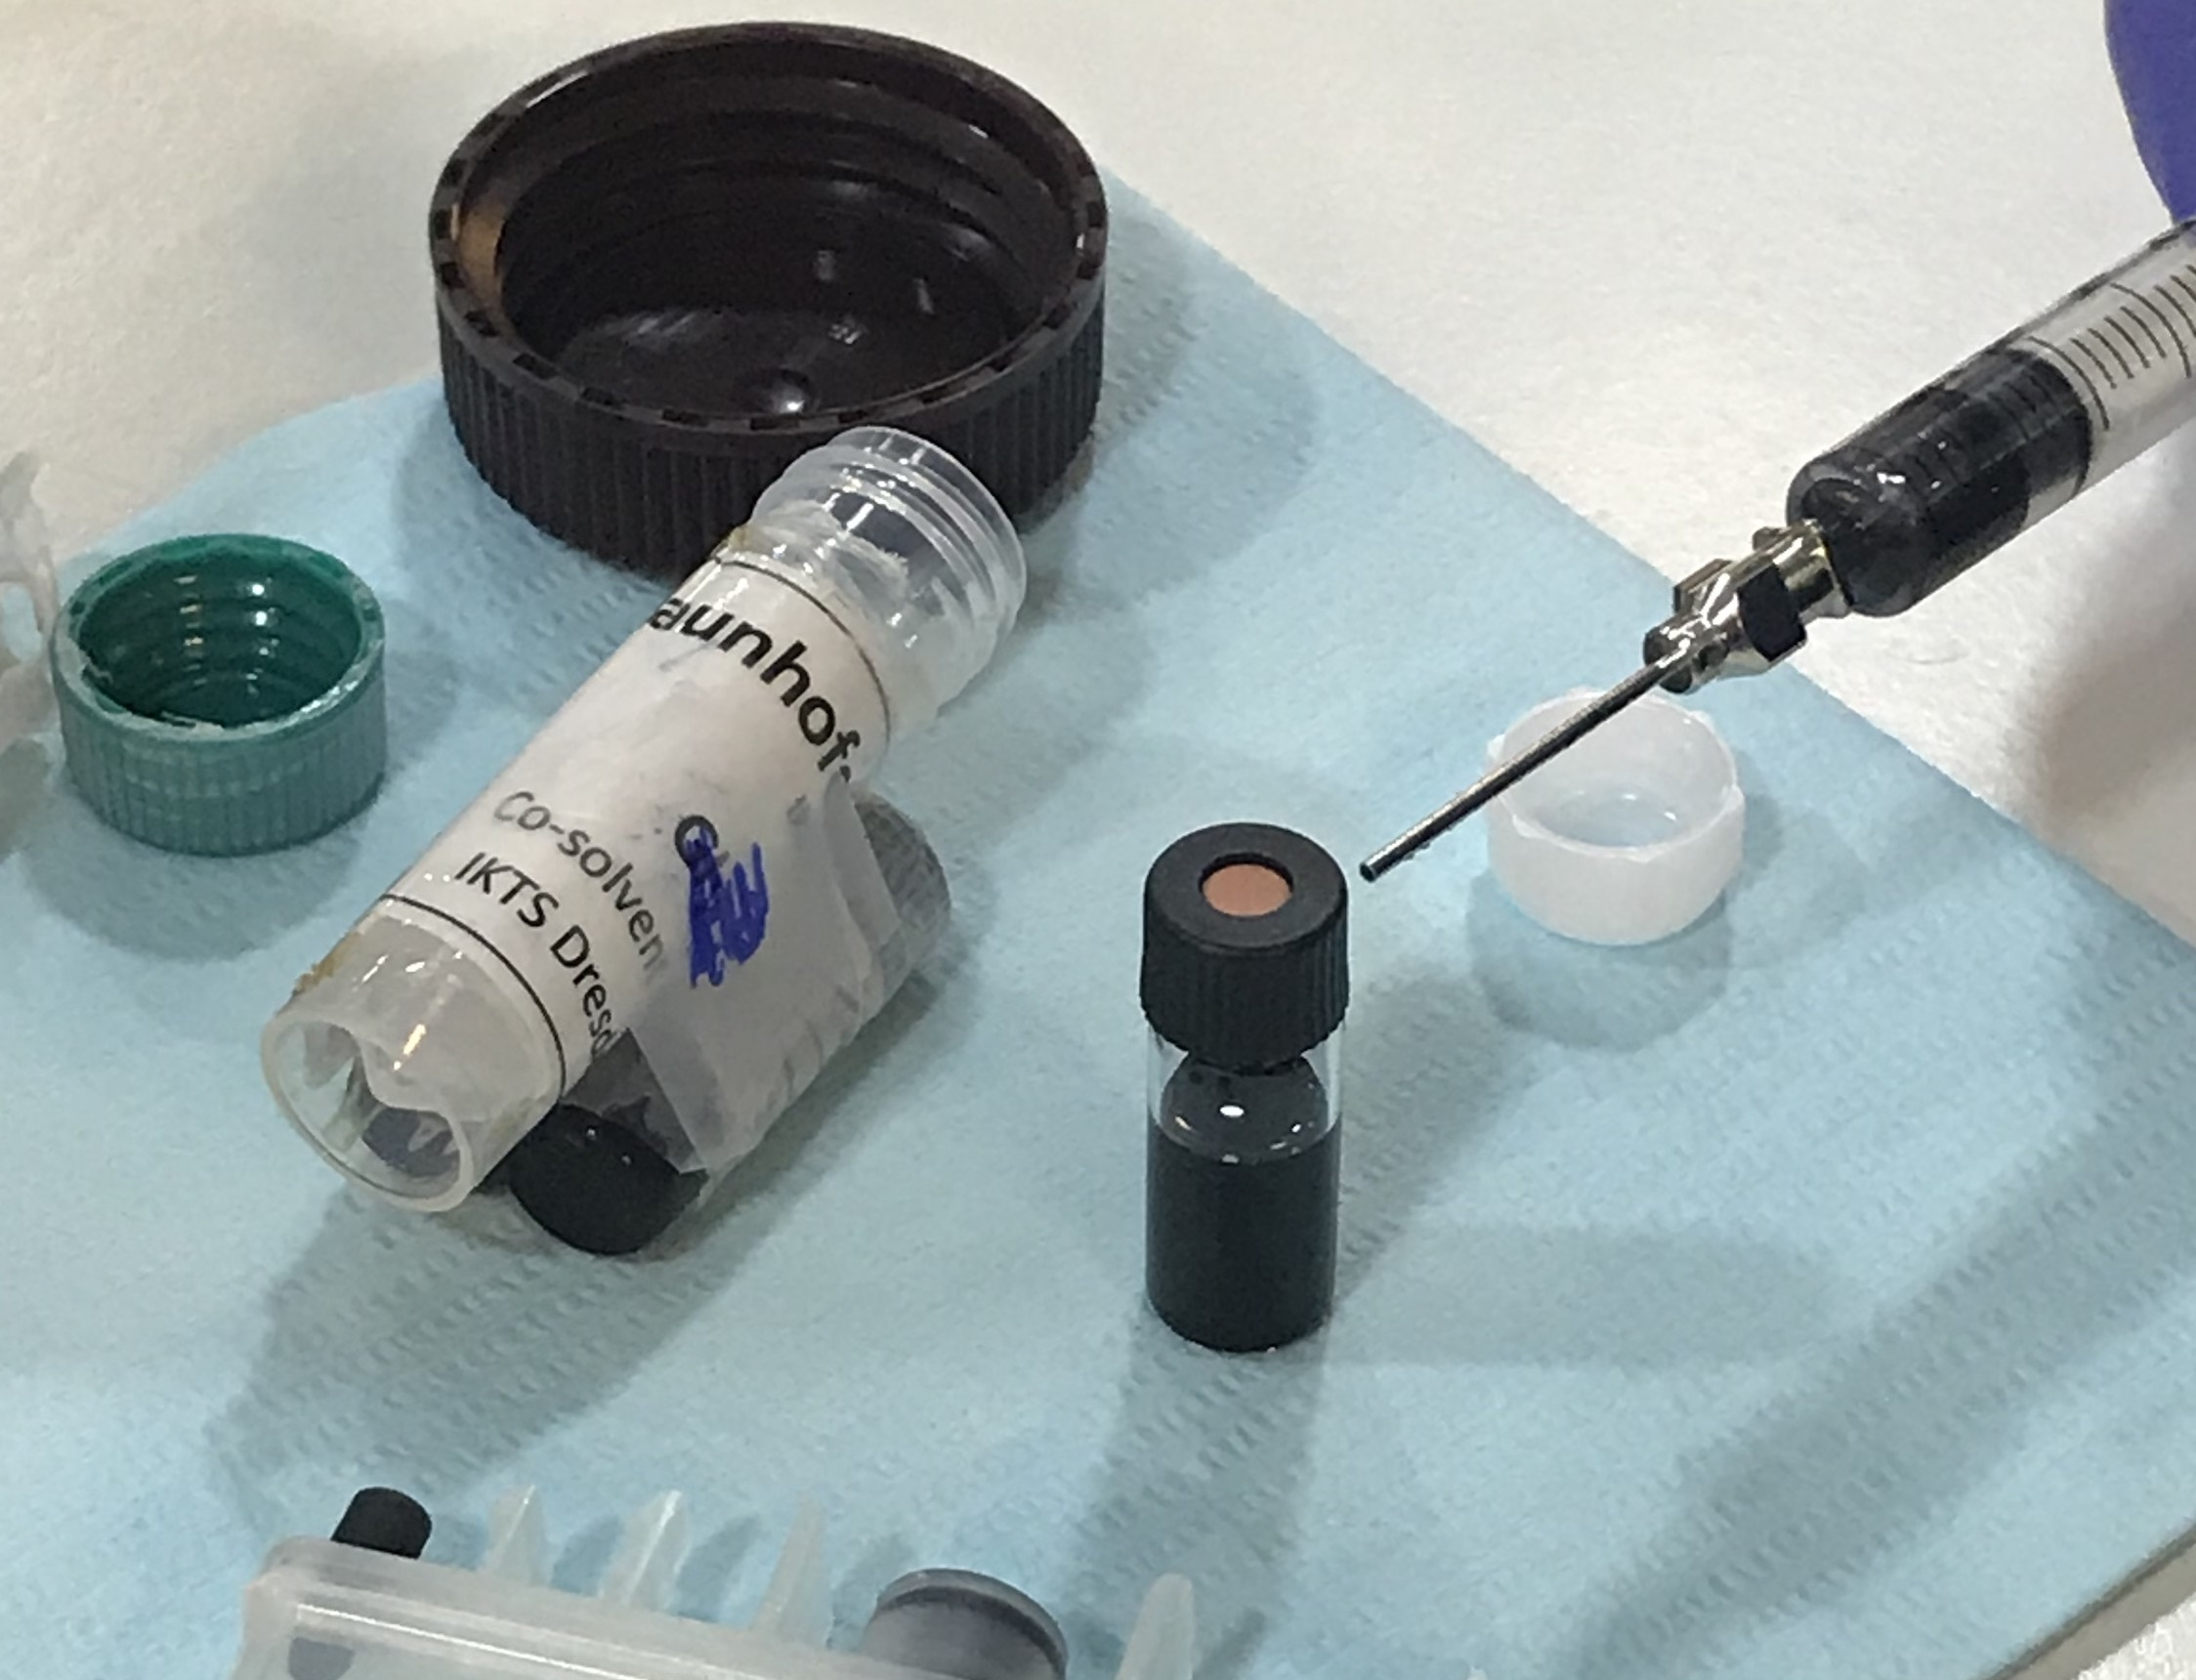
\includegraphics[width=0.5\textwidth]{Figures/Figura_tinta_Au}
  \caption{Hermetically sealed container with gold nanoparticle ink.}
  \label{fig:Figura_tinta_Au}
\end{figure}

\subsection{Photo-definable dielectric ink SU-8}
The dielectric ink used in this project is \emph{PriElex SU-8 2007} from \emph{MicroChem}. It is based on the SU-8 compound, is compatible with Inkjet printing processes and can be thermally cured without the need for UV exposure. (Figure ~\ref{fig:Figura_tinta_SU8}).

Some of its most outstanding advantages are its low curing temperature ($<$ 150ºC), excellent thermal stability and high chemical resistance.

It has a surface tension of 30 dynes/cm, a density of 1,038 g/cm\textsuperscript{3} and a kinematic viscosity of 9.33 cSt. These properties are reported in the manufacturer's datasheet \cite{PriElexSU8}.

\begin{figure}[H]
  \centering
    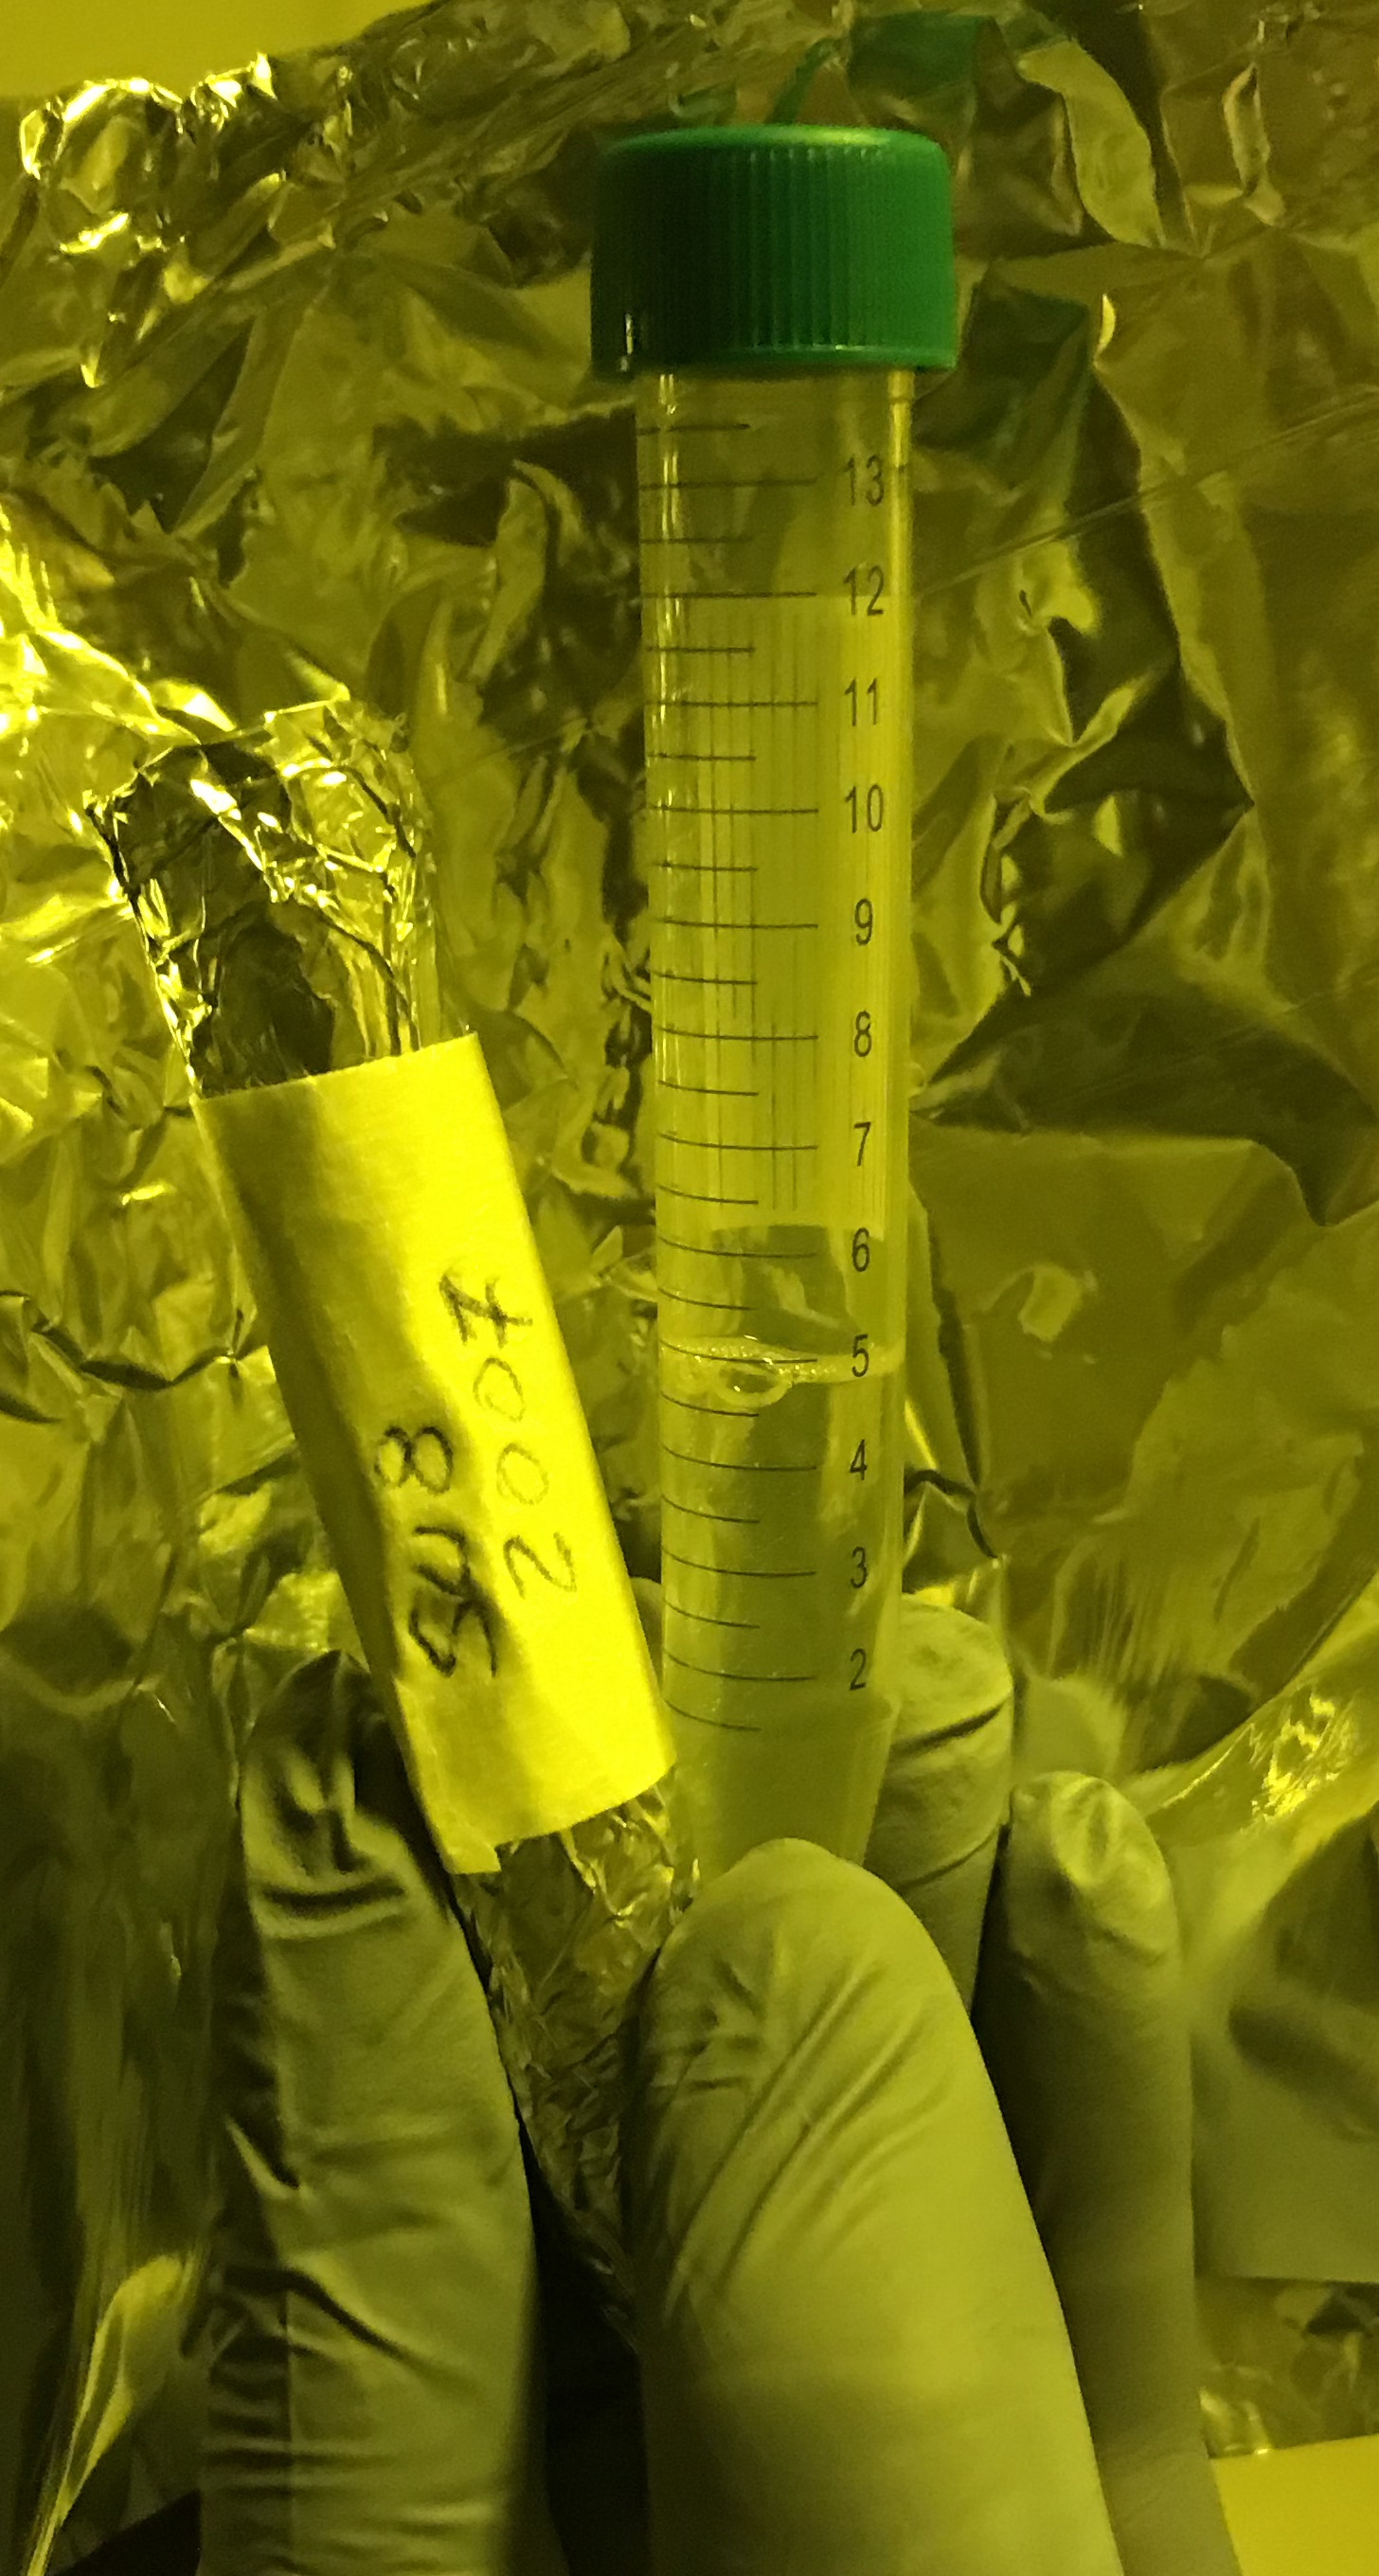
\includegraphics[width=0.2\textwidth]{Figures/Figura_tinta_SU8}
  \caption{SU-8 dielectric ink container.}
  \label{fig:Figura_tinta_SU8}
\end{figure}

\subsection{\textit{Valox} substrate}
The substrate, where the biosensors will be printed, is a film of terephthalite and thermoplastic polybutylene. It is marketed in different thicknesses, for this project the 600 $\mu$m one was used (Figure ~\ref{fig:Figura_Valox}).

This compound has excellent dielectric strength and is easy to handle for thermoforming, stamping, and bending, making it suitable for a wide range of electrical, electronic, and medical applications \cite{Valox}.

\begin{figure}[H]
  \centering
    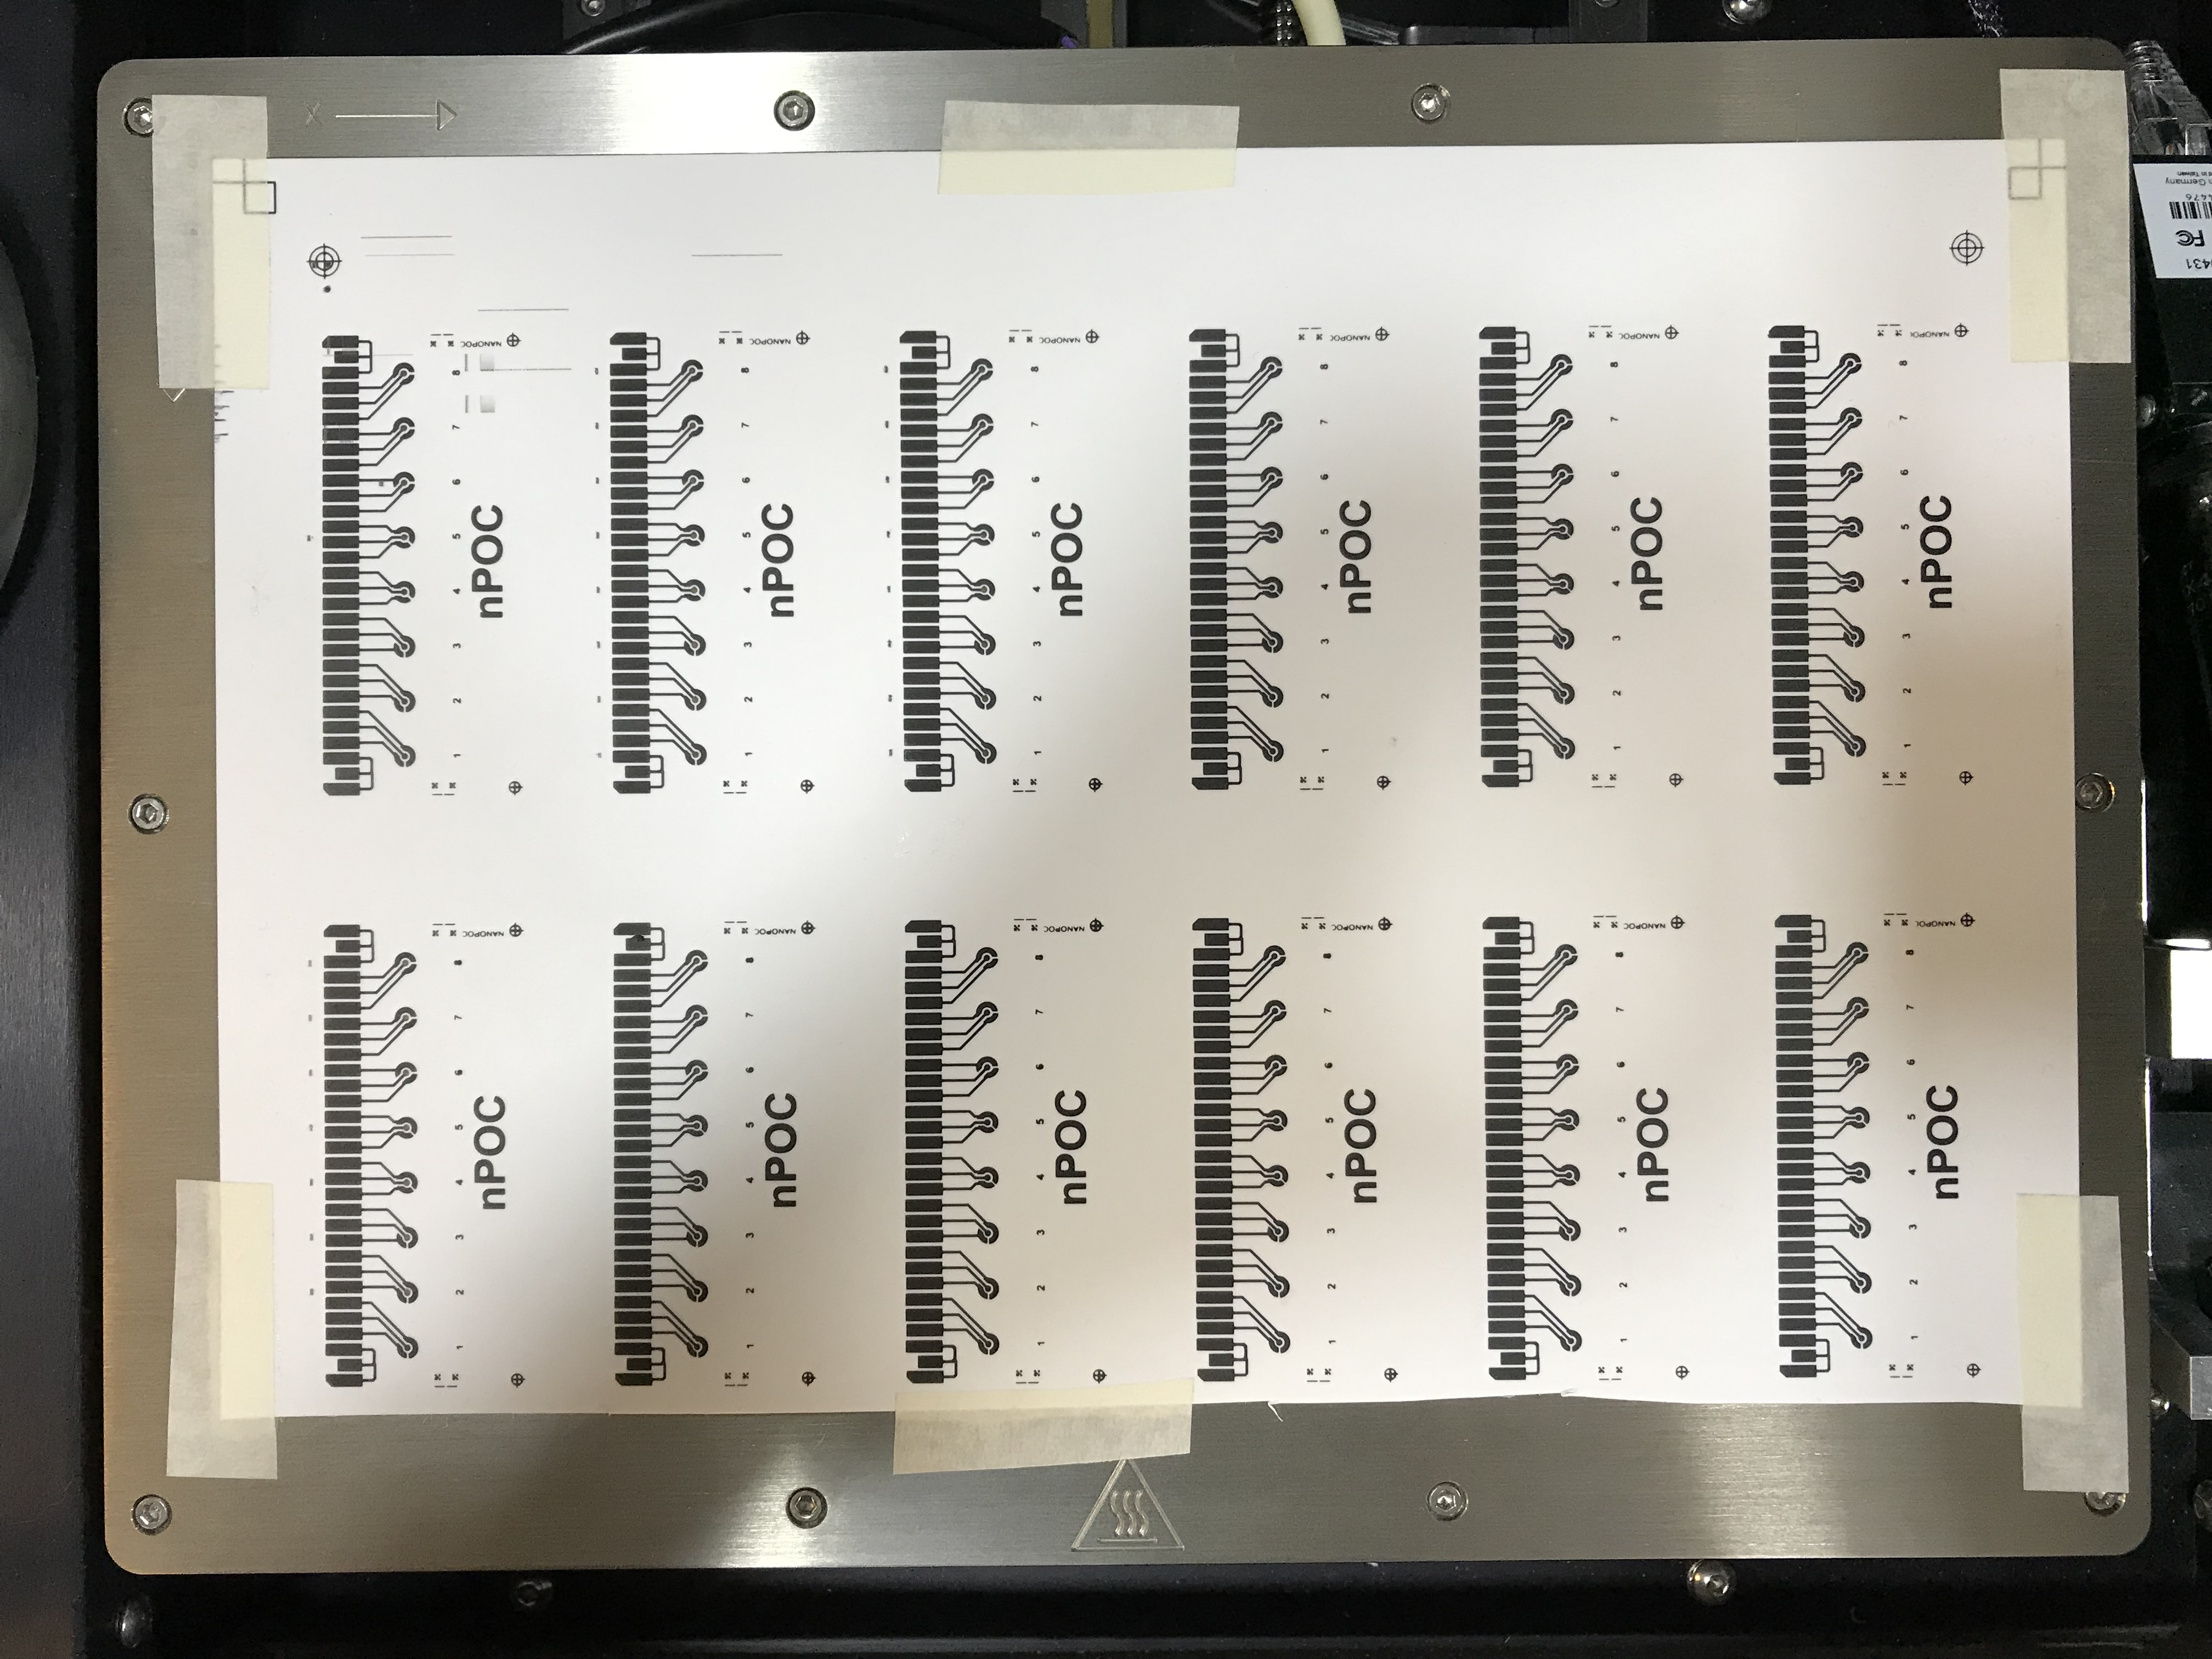
\includegraphics[width=0.55\textwidth]{Figures/Figura_Valox}
  \caption{\textit{Valox} substrate with carbon screen printing.}
  \label{fig:Figura_Valox}
\end{figure}

\section{Characterization techniques}
\subsection{Electrical Characterization}\label{subsec:carac_elec}
Due to the scale at which the nanoparticle ink is printed, it can have microcracks invisible to the eye or low magnification images, however, they are noticeable in microscope magnified images (Figure ~\ref{fig:Figura_Carac_elec}).

\begin{figure}[H]
  \centering
    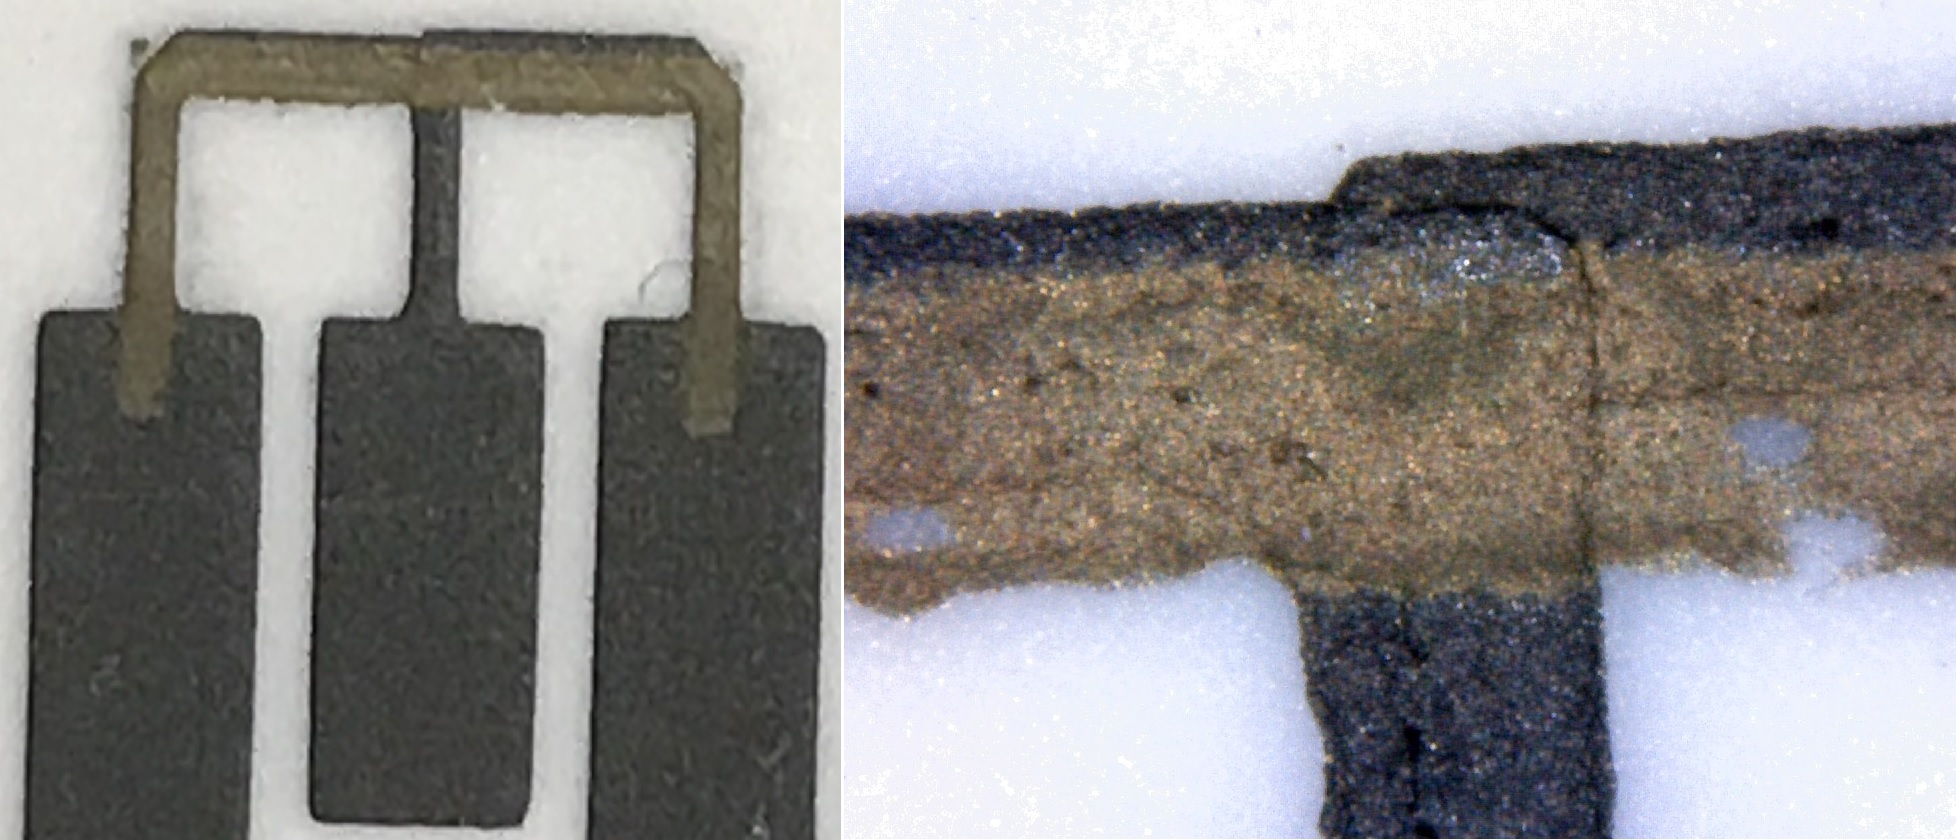
\includegraphics[width=0.5\textwidth]{Figures/Figura_Carac_elec}
  \caption{Image of conventional phone camera (iPhone 7) and image of USB microscope with 1000X Magnification.}
  \label{fig:Figura_Carac_elec}
\end{figure}

Through a 4-point resistance measurement (known as Kelvin method), the physical continuity of the film, the correct operation of the printer and therefore the biosensor working electrode can be ensured.

The method uses two circuits linked by a direct current source. The current from the source flow through one circuit is measured by an ammeter and the other has a voltmeter in parallel with the resistance to be measured. There is also a dual system to the previous one, where there is a verified voltage source with a voltmeter and an ammeter that measures the circulating current through the resistance (Figure ~\ref{fig:Figura_metodo_Kelvin}).

\begin{figure}[H]
  \centering
    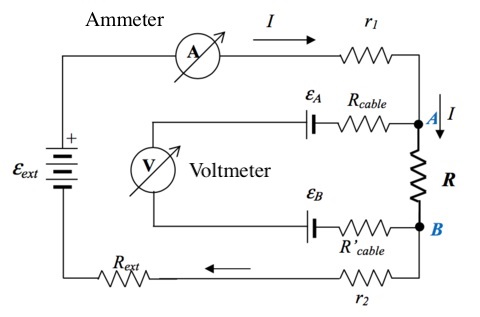
\includegraphics[width=0.5\textwidth]{Figures/Figura_metodo_Kelvin}
  \caption{Four-point measurement circuit.}
  \label{fig:Figura_metodo_Kelvin}
\end{figure}

\subsection{Optical/Dimensional Characterization}
As part of an optical or dimensional characterization it is important to know sizes, thicknesses and roughness.

Sizes can be obtained through the printer's fiducial camera. The software allows measurements of distances between two points and thus obtain all the values required in the characterization (Figure ~\ref{fig:Figura_Cam_Fiducial_Medicion}).

\begin{figure}[H]
  \centering
    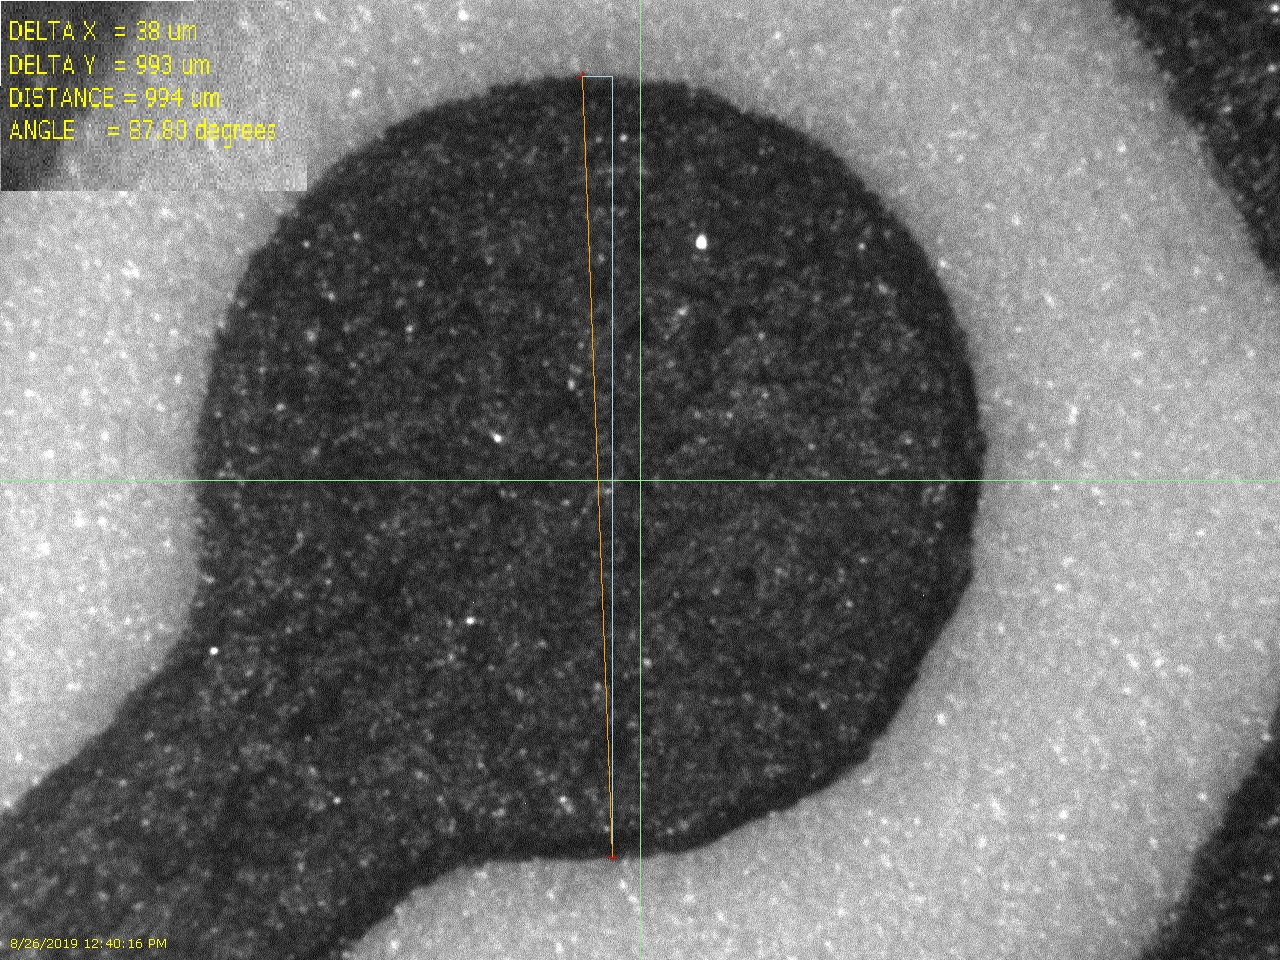
\includegraphics[width=0.5\textwidth]{Figures/Figura_Cam_Fiducial_Medicion}
  \caption{Fiducial camera image with distance measurement.}
  \label{fig:Figura_Cam_Fiducial_Medicion}
\end{figure}

The thickness of the impressions and the roughness of the surfaces can be obtained through a contact profilometer. This equipment, also called a roughness meter, uses a fine tip in contact with the surface to be analyzed (Figure ~\ref{fig:Figura_Stylus}), performing a controlled sweep in a straight line. The height variations detected by this tip are converted into electrical signals and can be recorded or graphed.

\begin{figure}[H]
  \centering
    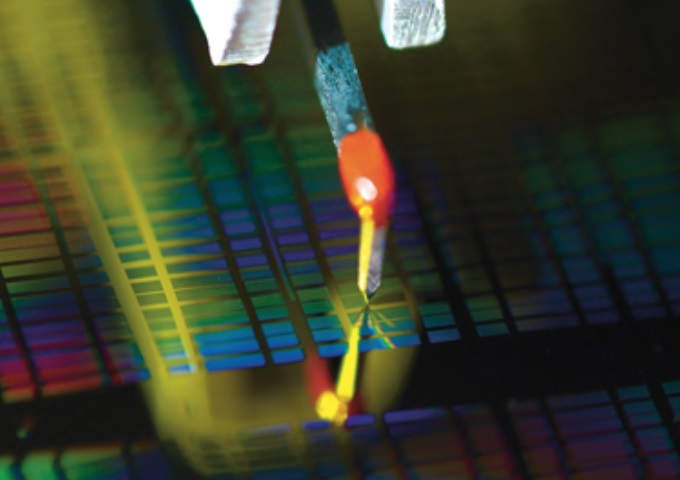
\includegraphics[width=0.5\textwidth]{Figures/Figura_Stylus}
  \caption{Stylus tip image of a contact profilometer.}
  \label{fig:Figura_Stylus}
\end{figure}

Roughness is an important data in characterization, since it defines the working effective area of the biosensor. The smoother the surface, the effective area will approach the geometric area of the electrode.

\subsection{Electrochemical Characterization}
For this work the direct current cyclic voltammetry procedure is used. This electrochemical characterization consists of varying, in a cyclical way, the electrical potential of the working electrode relative to a reference one. Both are immersed in a solution and the resulting current flowing through the working electrode is measured (Figure ~\ref{fig:Figura_circuito_voltametria}). 

\begin{figure}[H]
  \centering
    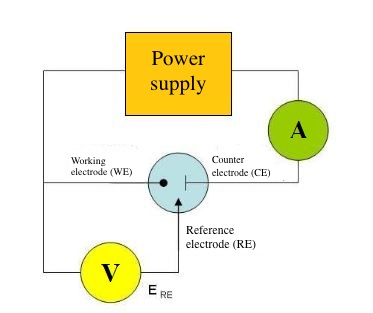
\includegraphics[width=0.65\textwidth]{Figures/Figura_circuito_voltametria}
  \caption{Electrical circuit diagram for direct current cyclic voltammetry.}
  \label{fig:Figura_circuito_voltametria}
\end{figure}

The excitation signal is a linear potential sweep with a triangular wave, which starts from an E1 potential, evolves linearly in time to an E2 potential and then returns to E1 (Figure ~\ref{fig:Figura_Carac_electroquimica}). The speeds of this sweep can range from less than 1 mV/s to hundreds of volts per second \cite{TesisGG}.

\begin{figure}[H]
  \centering
    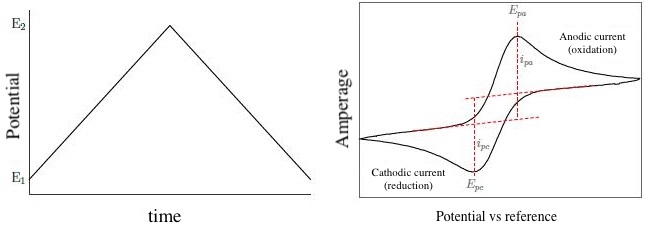
\includegraphics[width=1\textwidth]{Figures/Figura_Carac_electroquimica}
  \caption{Excitation curve and typical voltagram for a reversible redox species. Figure extracted from \cite{TesisGG}.}
  \label{fig:Figura_Carac_electroquimica}
\end{figure}

Ferrocyanide and ferricyanide were used as electrochemical probes. The choice of these probes is due to the reversibility of the \textit{redox} pairs, whose oxidized and reduced species are inexpensive and easy to obtain, soluble in aqueous solution and behave in a quasi-reversible way against electronic exchange.

In the simplest approximation, they are expected to follow the voltammetric behavior described by Randles-Sevcik \ref{ecuacion3}, where the peak current $(i_{p})$ is proportional to the concentration (C), to the square root of the sweep speed (\textit{v}) and to the area (A). The other parameters are considered constant.

\begin{equation}\label{ecuacion3}
i_{p}=0,4463 n F A C \left( \frac{nFvD}{RT} \right) ^{1/2}\
\end{equation}
\chapter{Experimental development}
For the following project, Valox substrate with screenprinted carbon electrochemical cells were used as base (Figure ~\ref{fig:Figura_Electrodos_nPOC}). A Fujifilm printer model Dimatix DMP-2850 was used to deposit the ink of gold on the working electrode. Its electrical, dimensional and electrochemical properties were characterized to corroborate the correct operation of the sensors.

\begin{figure}[H]
  \centering
    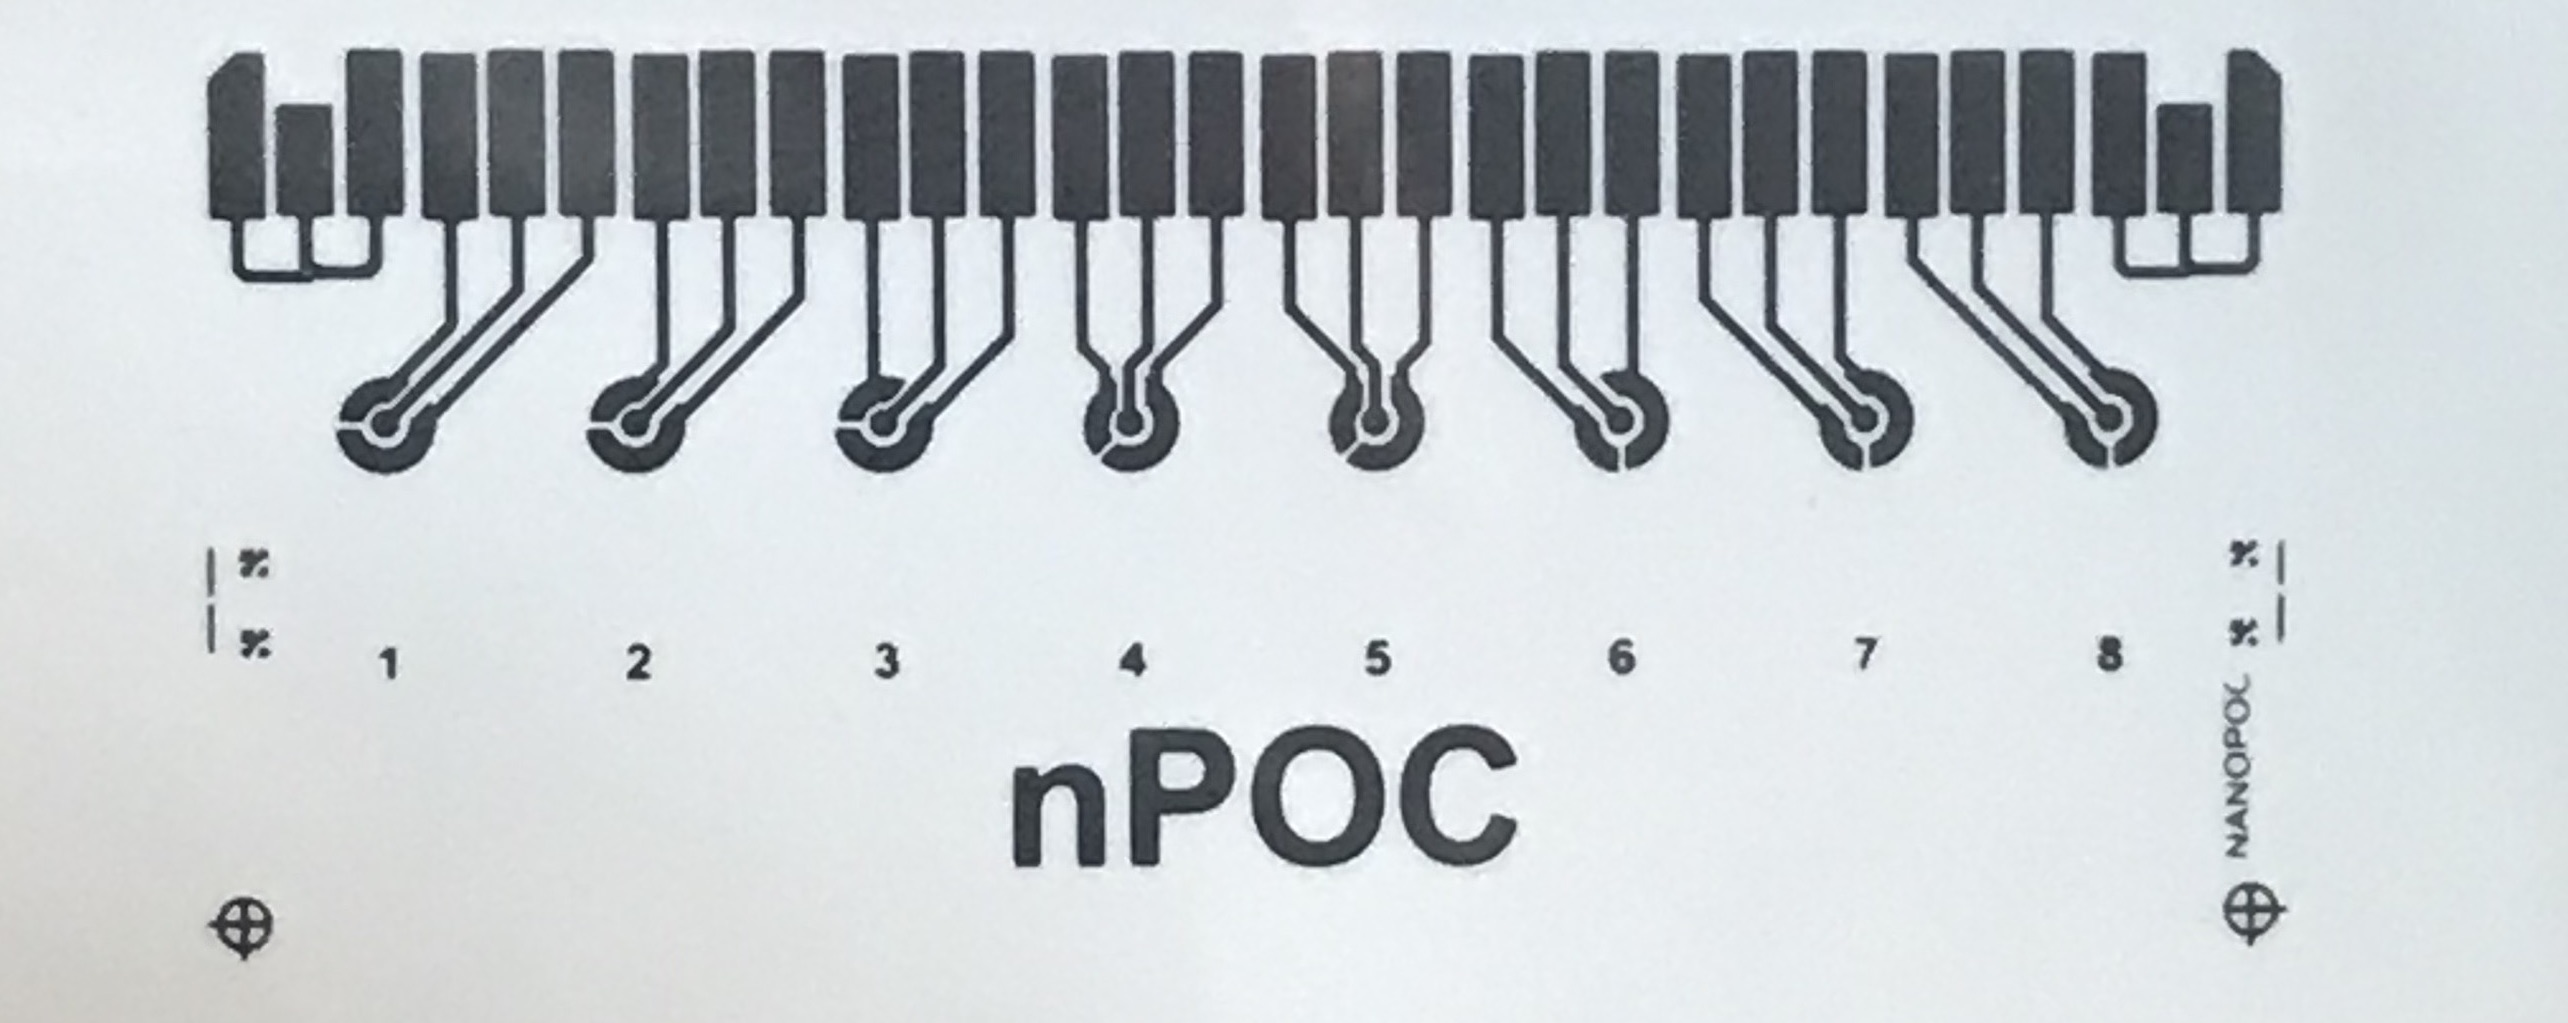
\includegraphics[width=0.5\textwidth]{Figures/Figura_Electrodos_nPOC}
  \caption{Electrochemical Cells}
  \label{fig:Figura_Electrodos_nPOC}
\end{figure}

\section{Preparation of image patterns}

\subsection{Preliminary measurements}
As a first instance, the different components of carbon printed electrochemical cells were measured. It was concluded that the working electrodes (from now on \emph{WE}) have a diameter of 1 mm, where the gold ink will be deposited. The separation between \emph{WE} and reference electrode (from now \emph{RE}) and counter electrode (from now \emph{CE}) is 400 $\mu$m. The distance between two \emph{WE} is 9 mm and each cartridge has eight sensors. This measured distance between two \emph{WE} corresponds to the separation of an eight-channel micro pipette, used in laboratories. (Figure ~\ref{fig:Figura_medicion_celdas})

\begin{figure}[H]
  \centering
    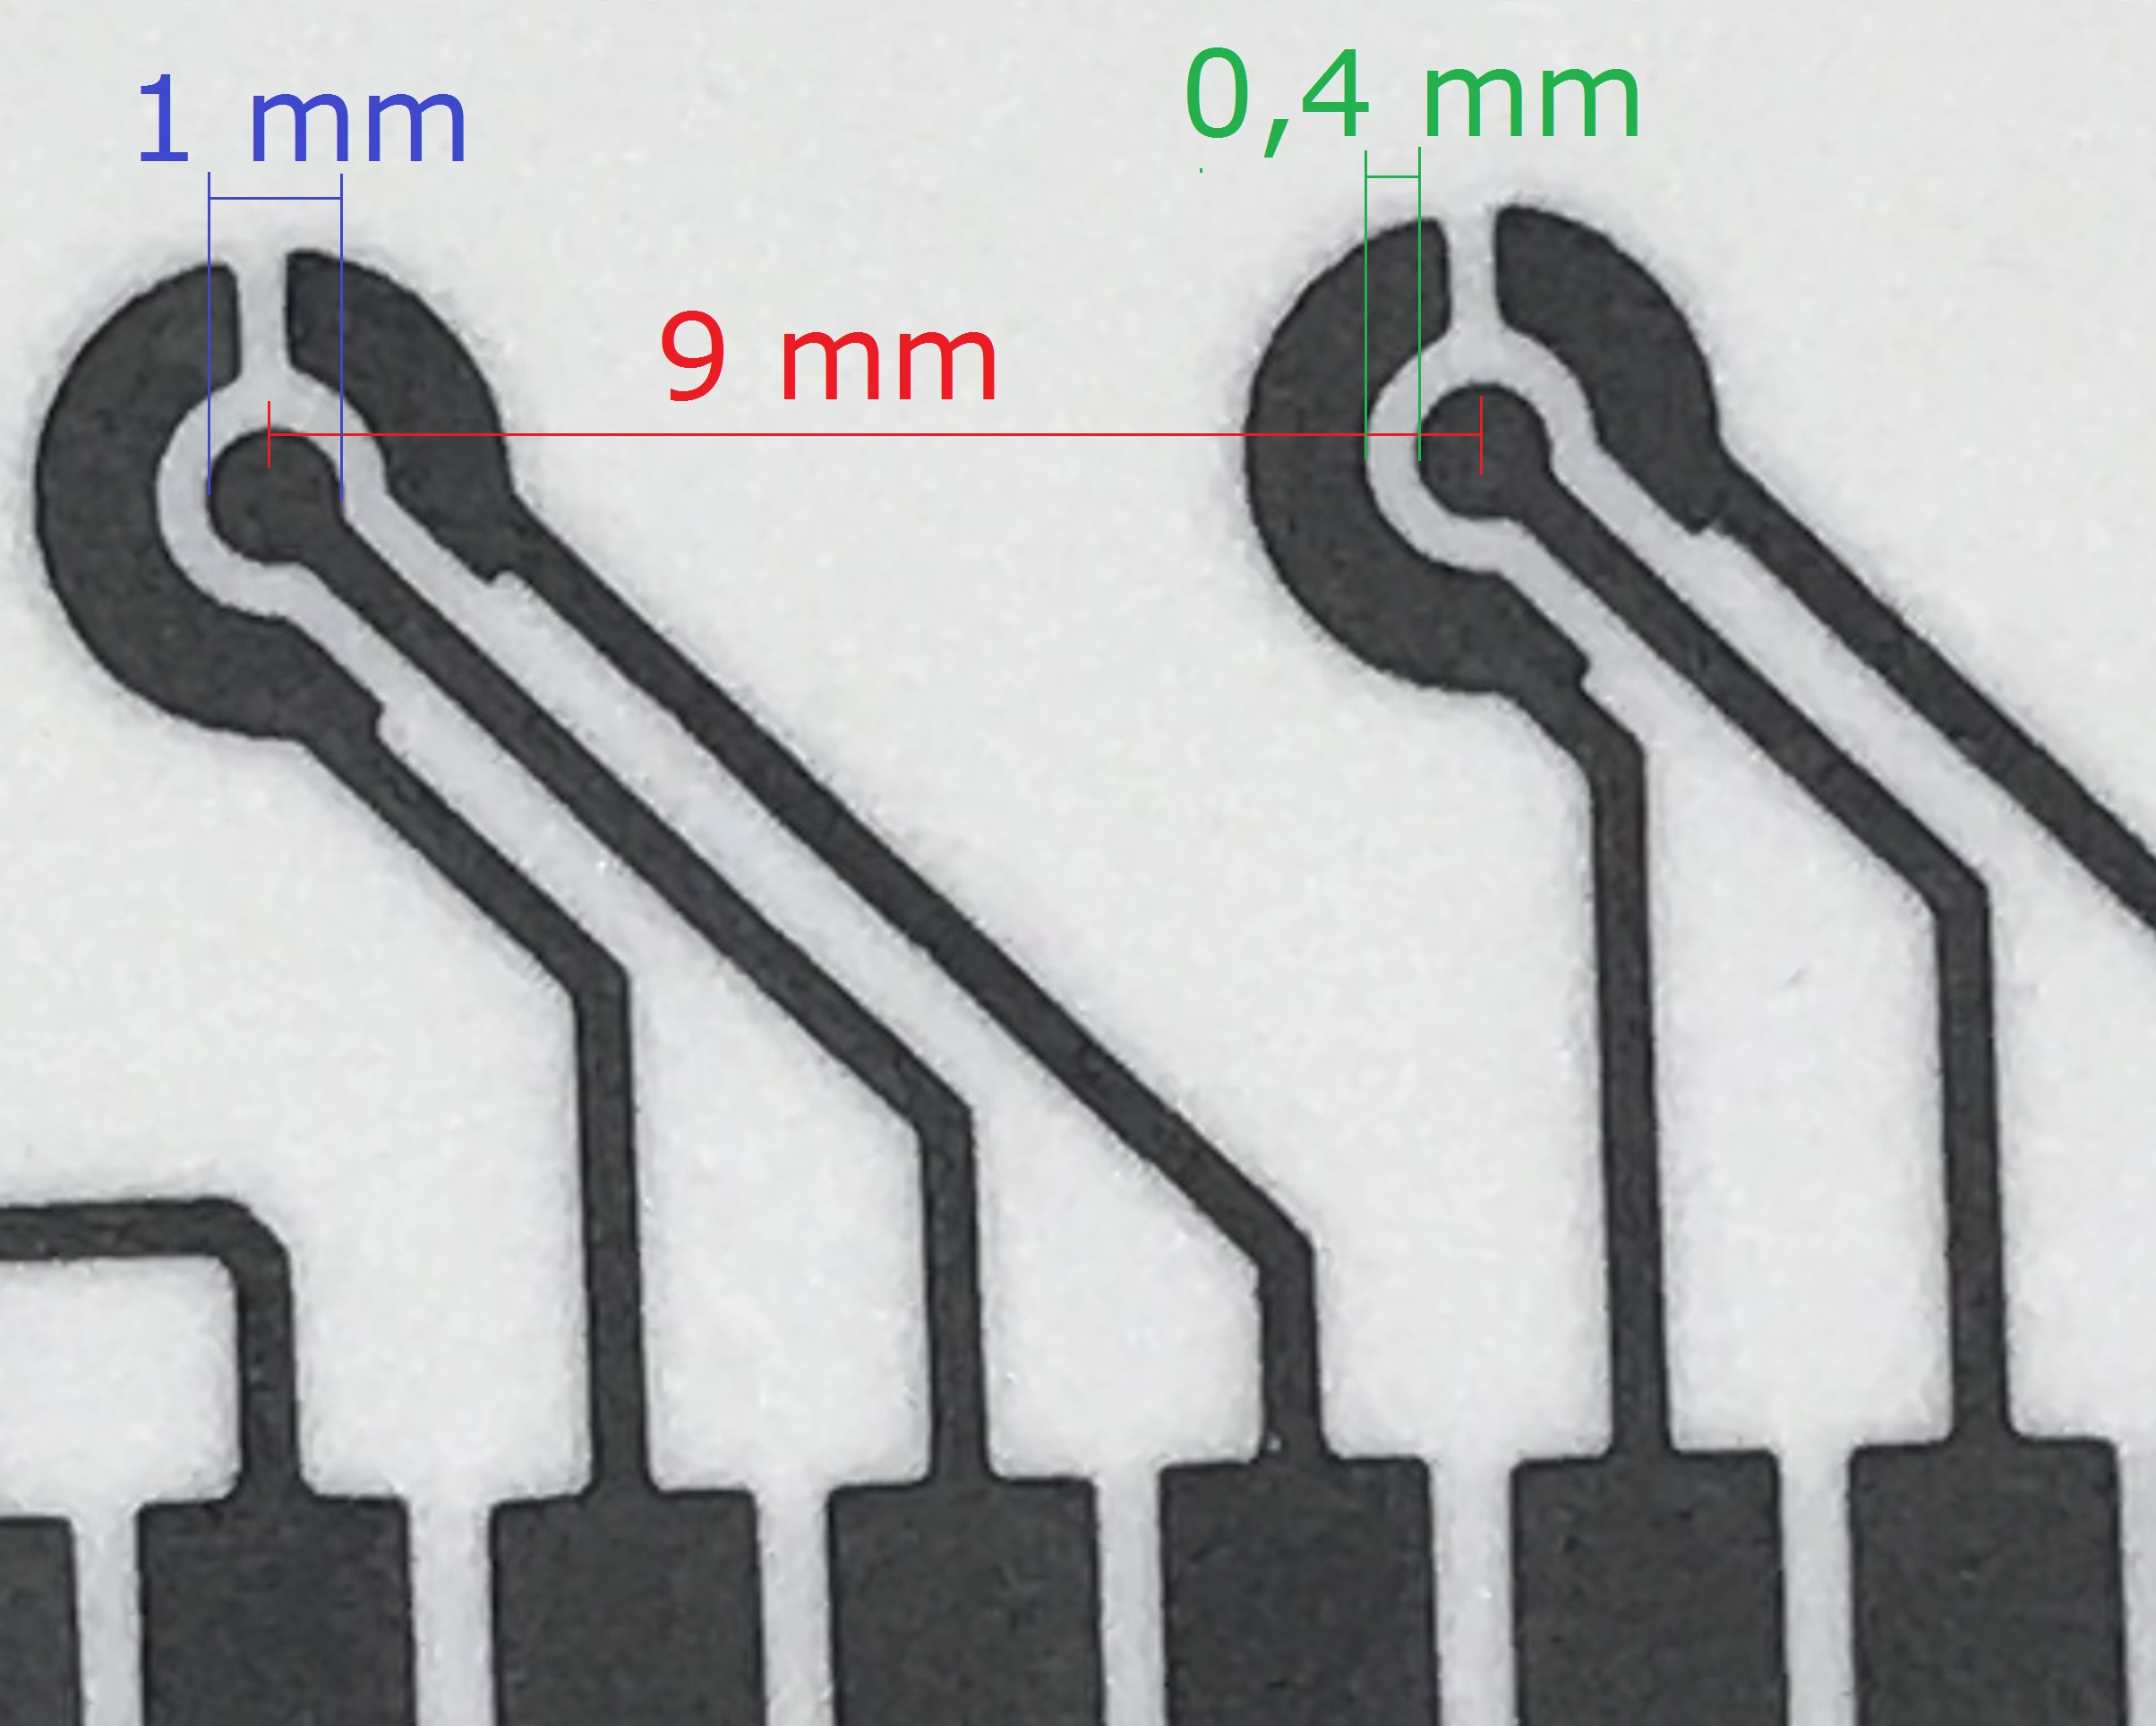
\includegraphics[width=0.5\textwidth]{Figures/Figura_medicion_celdas}
  \caption{Dimensional measurements on substrate.}
  \label{fig:Figura_medicion_celdas}
\end{figure}

Since the carbon prints were made by a company dedicated to industrial screen printing, the biosensors are manufactured in two columns and six rows giving a total of twelve sensors per substrate of A4 size (Figure ~\ref{fig:Figura_sensores_hoja_A4}). To have an accurate follow-up of the work to be carried out on each sample, they are listed taking advantage of their already printed carbon name as \textit{nPoc} from 1 to 5. (Figure ~\ref{fig:Figura_ejemplo_numeracion_nPoc})

\begin{figure}[H]
  \centering
    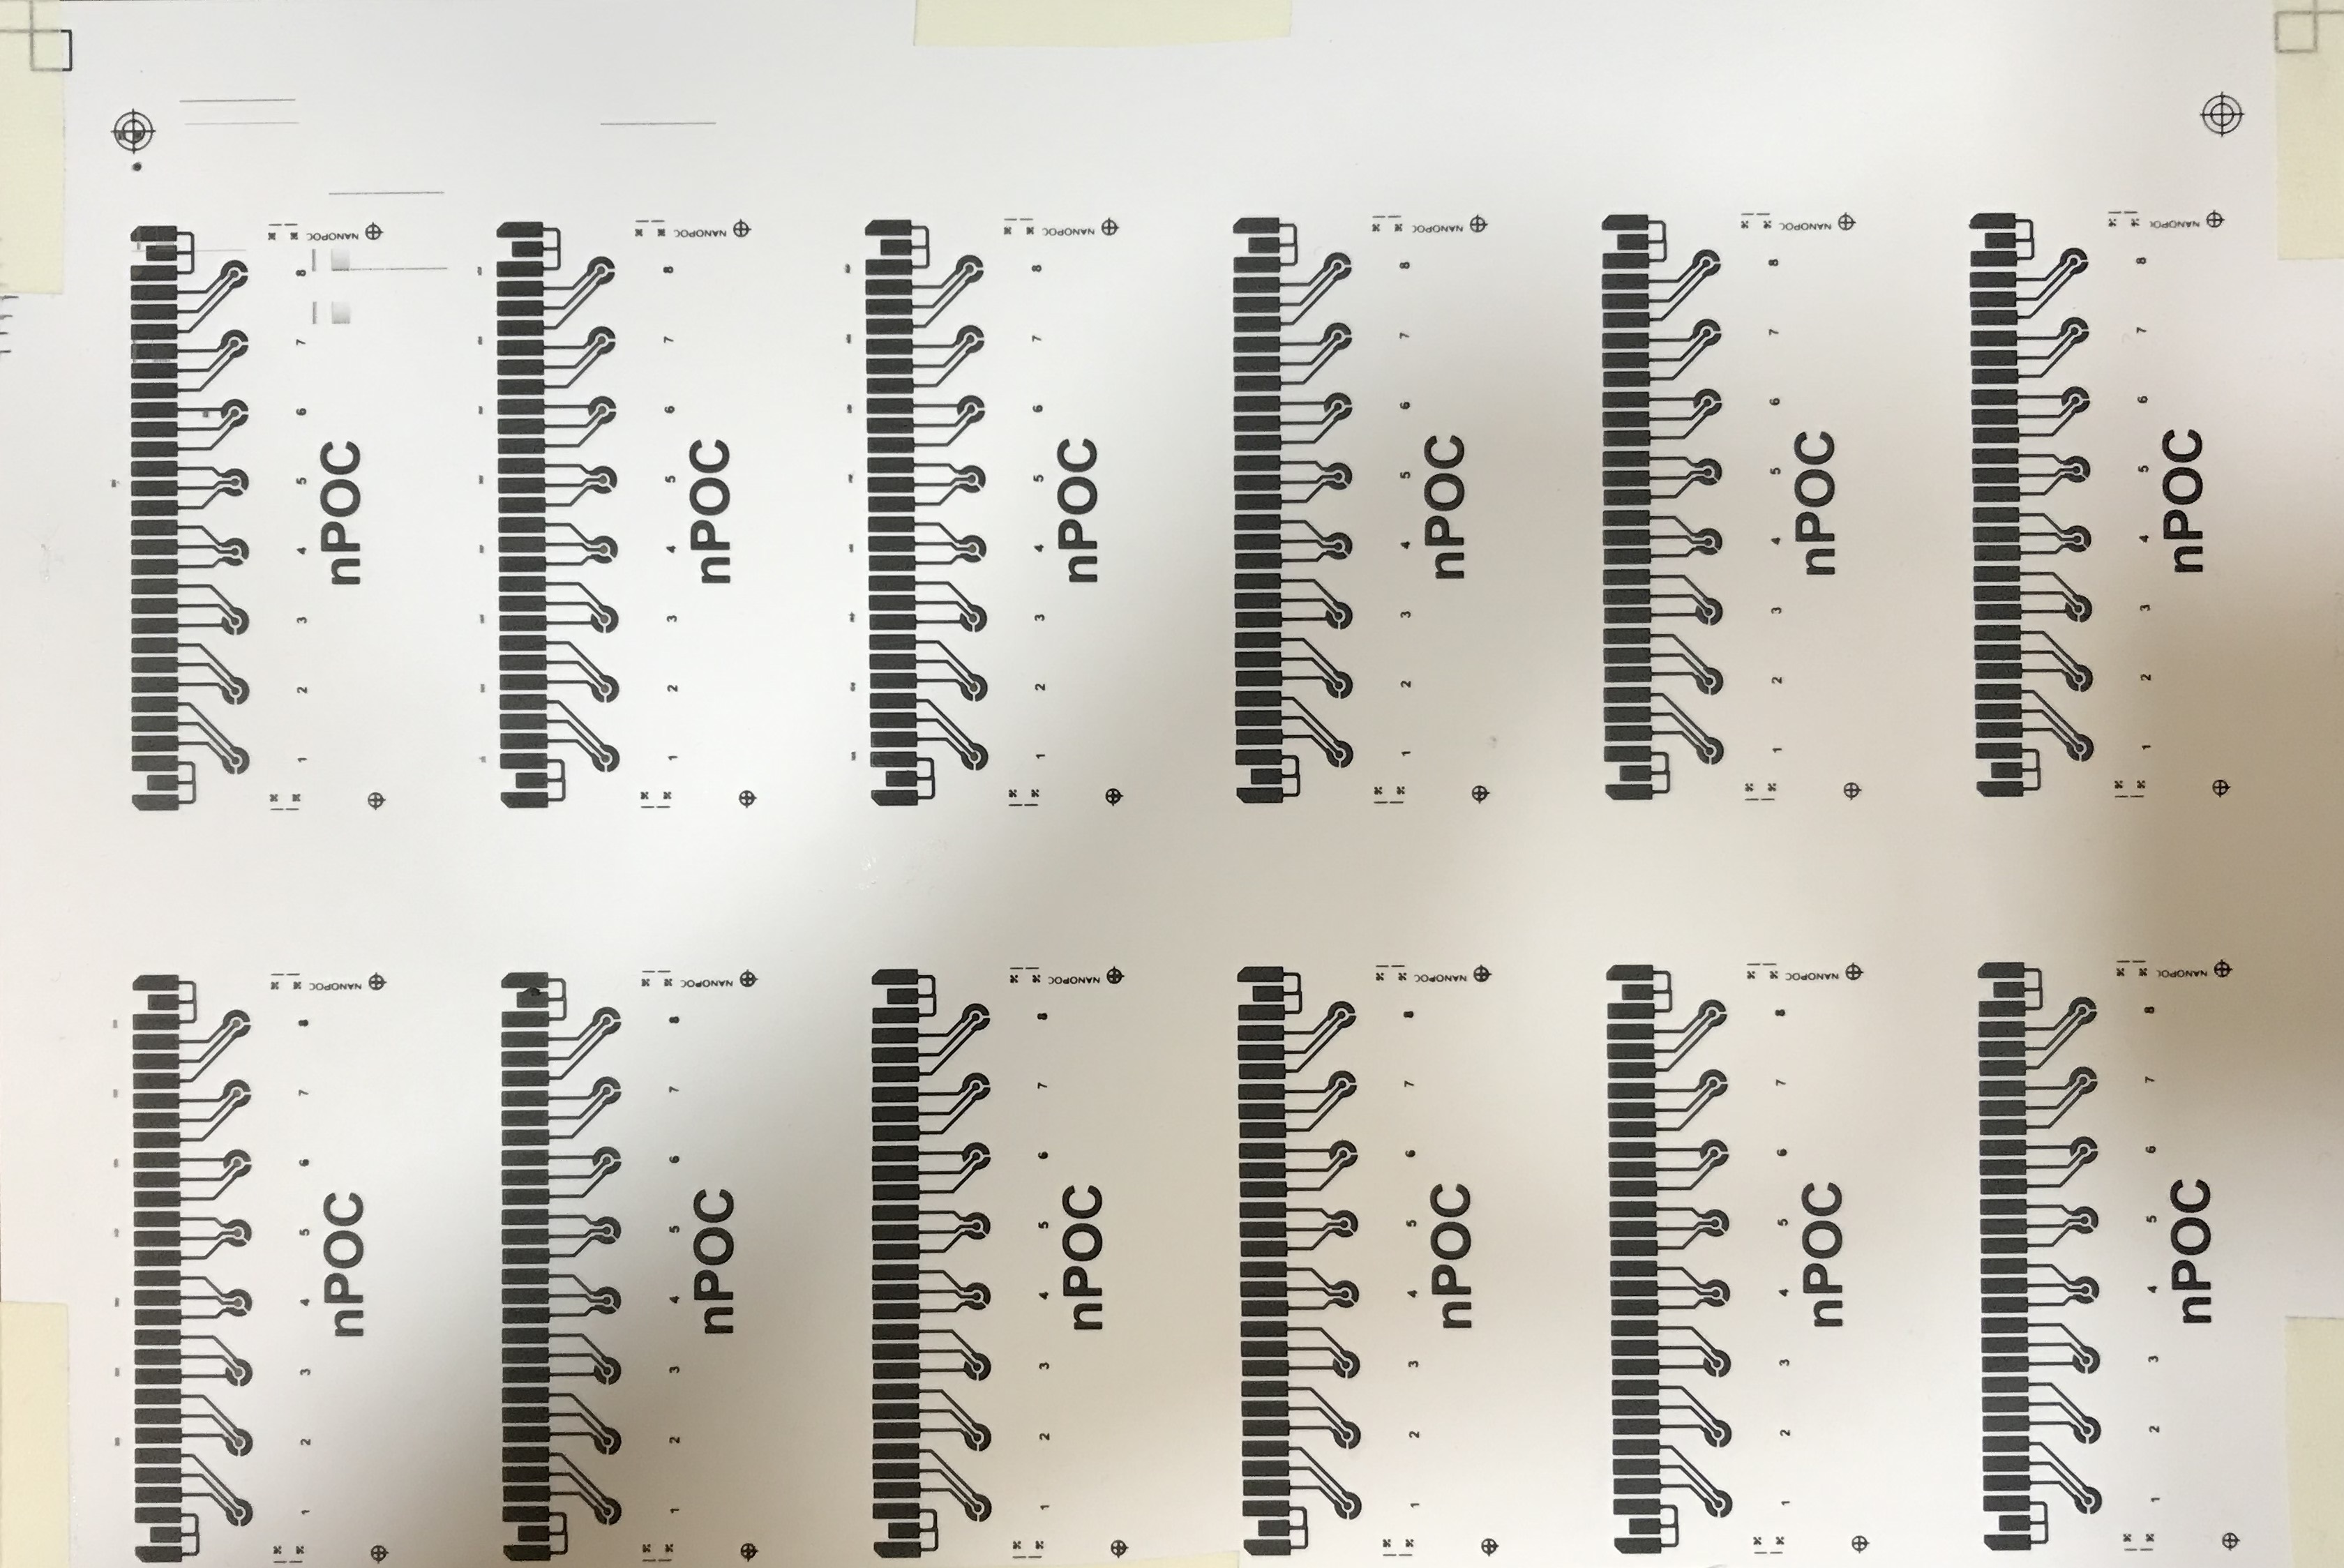
\includegraphics[width=0.5\textwidth]{Figures/Figura_sensores_hoja_A4}
  \caption{Screen printing of biosensors on A4 sheet.}
  \label{fig:Figura_sensores_hoja_A4}
\end{figure}

\begin{figure}[H]
  \centering
    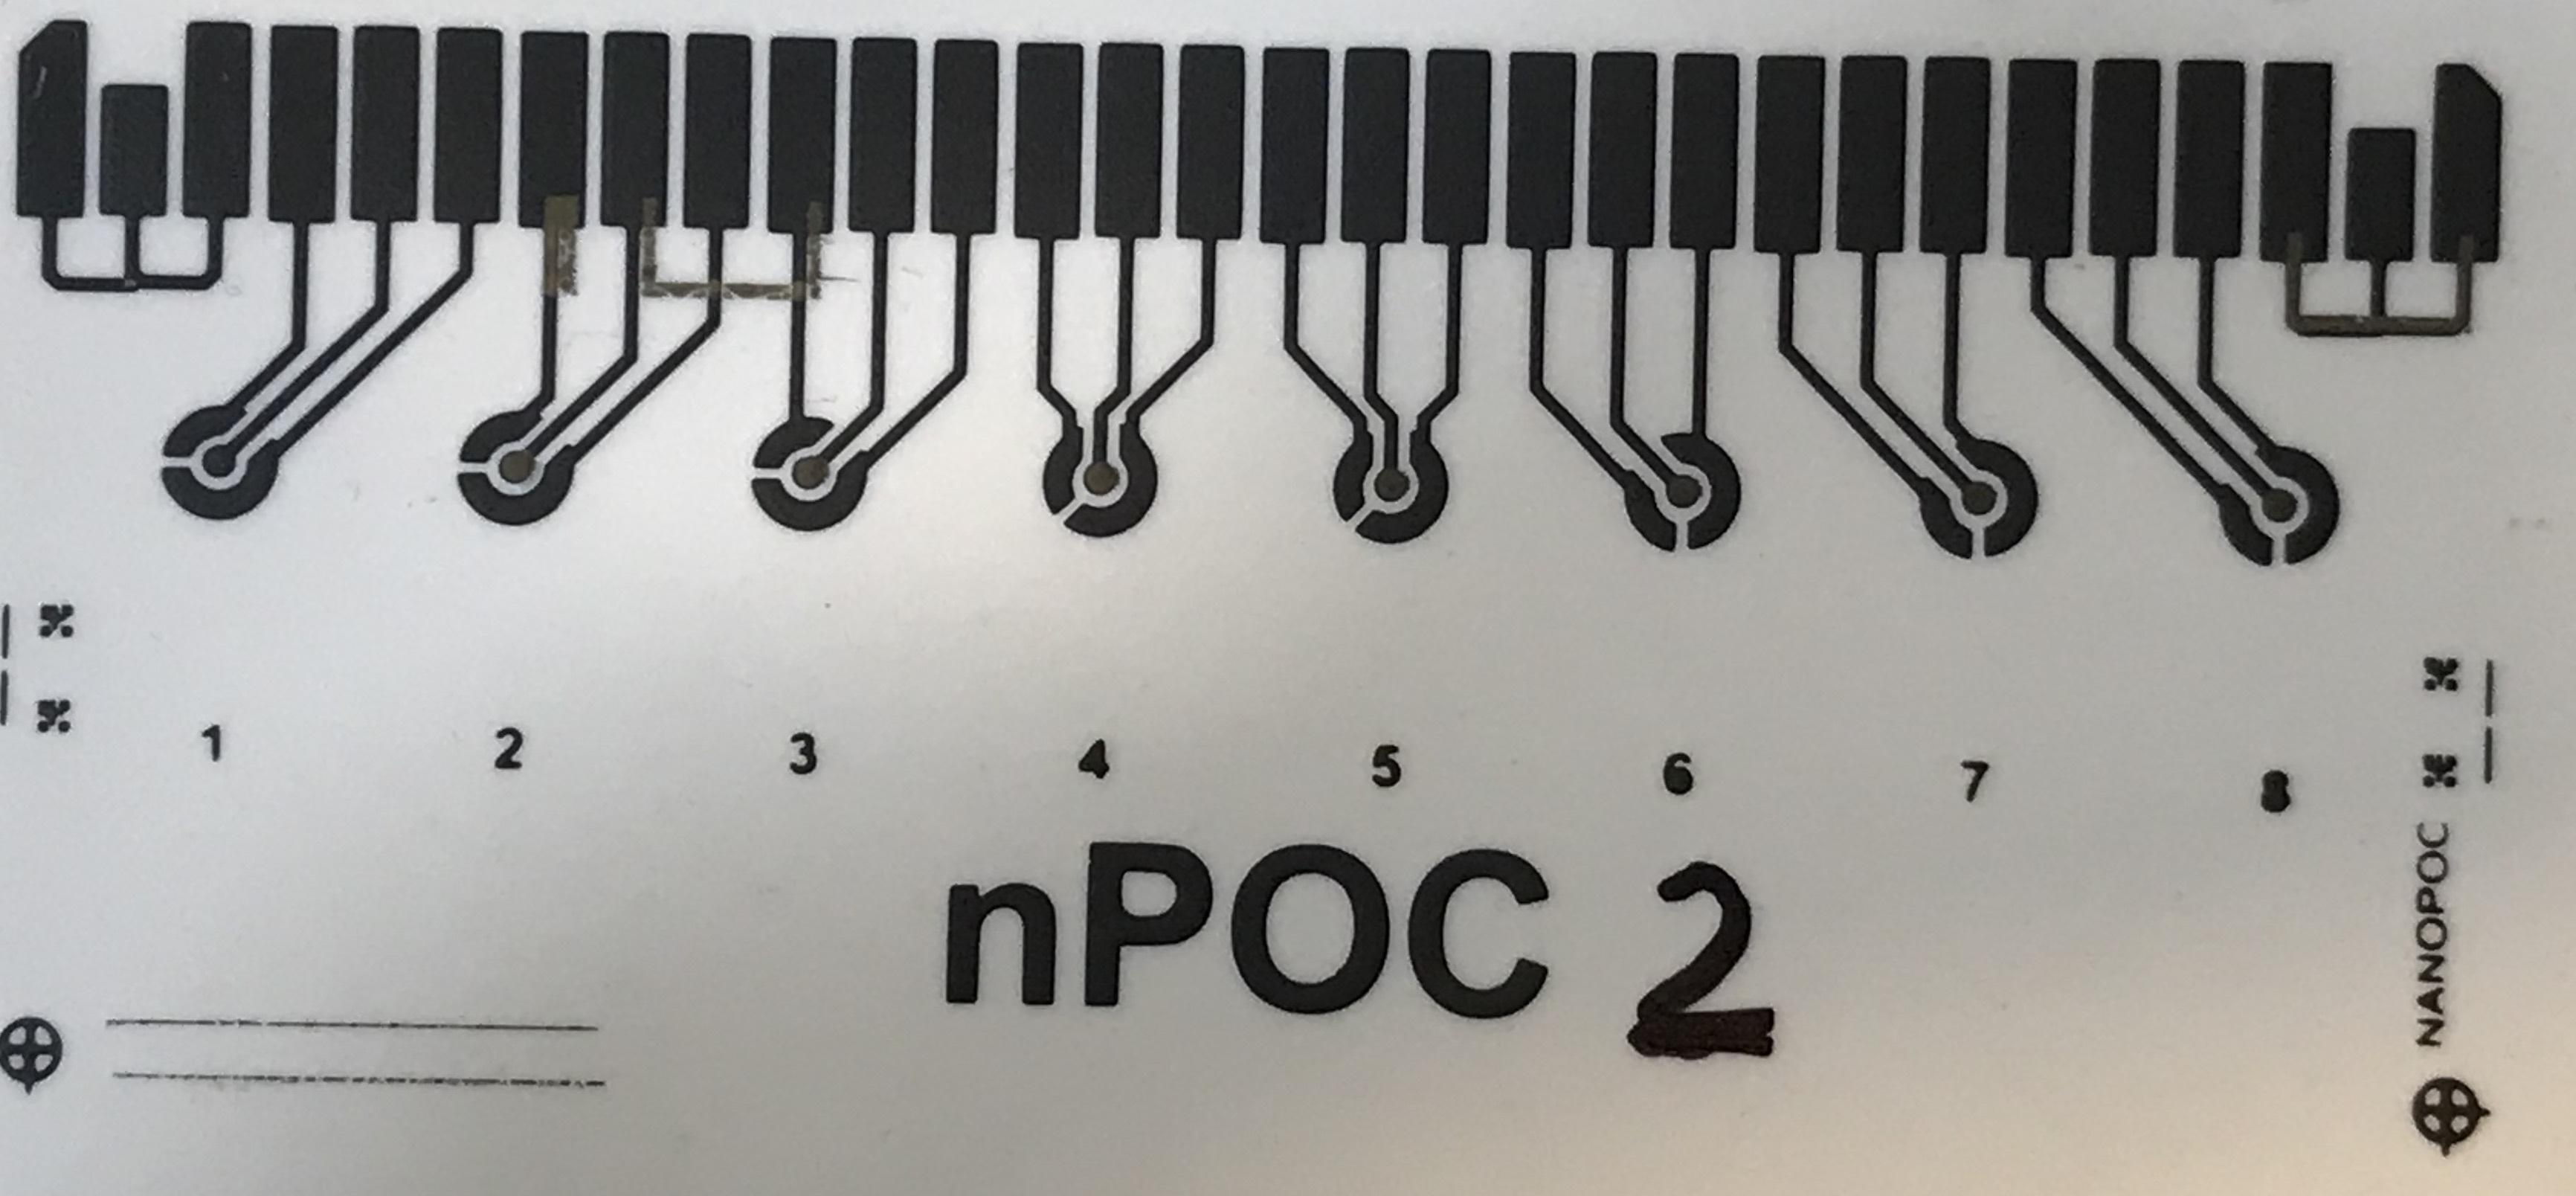
\includegraphics[width=0.5\textwidth]{Figures/Figura_ejemplo_numeracion_nPoc}
  \caption{nPoc2 sensor numbering example.}
  \label{fig:Figura_ejemplo_numeracion_nPoc}
\end{figure}

\subsection{Print pattern designs}
\label{subsec:diseno_impresion}
Once the necessary measurements have been obtained from the sensors, the printing patterns are designed. The professional free and open source InkScape graphic vector editor was used for this \cite{Inkscape} (Figure ~\ref{fig:Figura_Inkscape}).

\begin{figure}[H]
  \centering
    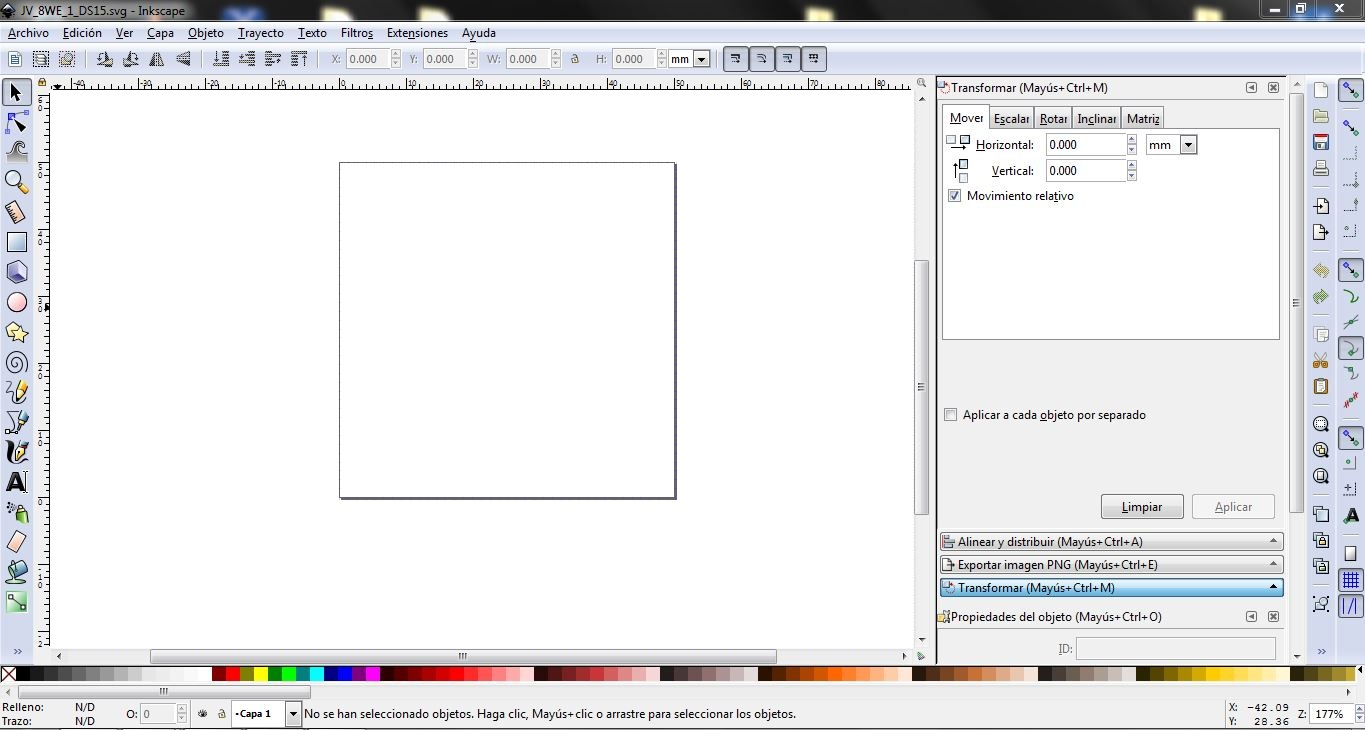
\includegraphics[width=0.65\textwidth]{Figures/Figura_Inkscape}
  \caption{Free and open source professional graphic vector editor.}
  \label{fig:Figura_Inkscape}
\end{figure}

Four drawings were made with two possible resolutions. The first drawings correspond to a circle of 1 mm and 1.1 mm in diameter, the size of one \emph{WE} and 100 $\mu$m more in the second. This is to establish whether using the same diameter achieves optimum coverage with the gold nanoparticle ink or if an offset needs to be added. The other two drawings consist of an array of eight 1 mm diameter circles spaced 9 mm apart and an array of eight 1.1 mm diameter circles with the same spacing (Figure ~\ref{fig:Figura_Diseno_Circulos}). The resolutions used were 1693.33 and 1270 dpi, later the reason for said resolutions will be explained.

\begin{figure}[H]
  \centering
    
\includegraphics[width=0.5\textwidth]{Figures/Figura_Diseno_Circulos}
  \caption{1 and 1.1 mm print designs.}
  \label{fig:Figura_Diseno_Circulos}
\end{figure}

Since the printer software (\textit{Dimatix Drop Manager}) does not detect color or grayscale images, they must be converted to monochrome 1-bit files. This way, the only thing present in the image are black or white pixels, corresponding to where a drop of ink should be ejected or not. The format that can save 1-bit images is the Windows bitmap (or BMP for its acronym in English), and therefore it is the only external format supported by the \textit{Dimatix Drop Manager}. Conversion to BMP format is done using \textit{Microsoft Paint} Software. By zooming in on the same image in PNG and BMP format, the differences can be seen with the naked eye (Figure ~\ref{fig:Figura_comparacion_png_bmp}).

\begin{figure}[H]
  \centering
    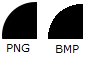
\includegraphics[width=0.5\textwidth]{Figures/Figura_comparacion_png_bmp}
  \caption{Comparison of PNG and BMP files.}
  \label{fig:Figura_comparacion_png_bmp}
\end{figure}

Once the files are obtained in the correct format, the printer parameters can be prepared and set up.

\section{Printer setup and calibration}
\label{sec:calib_impresora}
After preparing, placing and configuring the ink cartridge and the substrate (see \hyperref[chap:apendiceA]{Annex A}), the design or pattern to be printed must be added.

For this the DMP software offers two options. The first allows drawing with the same program, adding positions (X and Y coordinates) and the desired thickness; the second allows you to import images in monochrome BMP format. The creation of designs using the DMP software only allows basic shapes and, above all, shaped by straight lines. For more complex drawings, the external design procedure explained in the section on print pattern design is recommended (Chapter 3, \hyperref[subsec:diseno_impresion]{section 3.1.2}).

For any of the two options, reference coordinates can be added, used to locate the print on the substrate and a $``$\textit{Leader Bar}$``$ with the possibility of setting its width and its distance (\textit{Gap}) with the design to be printed. This last function is a commonly used procedure to keep the nozzles active and a uniform flight speed of the drops at the start of printing, improving the quality of the pattern. It must be taken into account that the $``$\textit{Leader Bars}$``$ must be located inside the substrate, otherwise ink will be being ejected onto the printer plate (Figure ~\ref{fig:Figura_Leader_Bar}).

\begin{figure}[H]
  \centering
    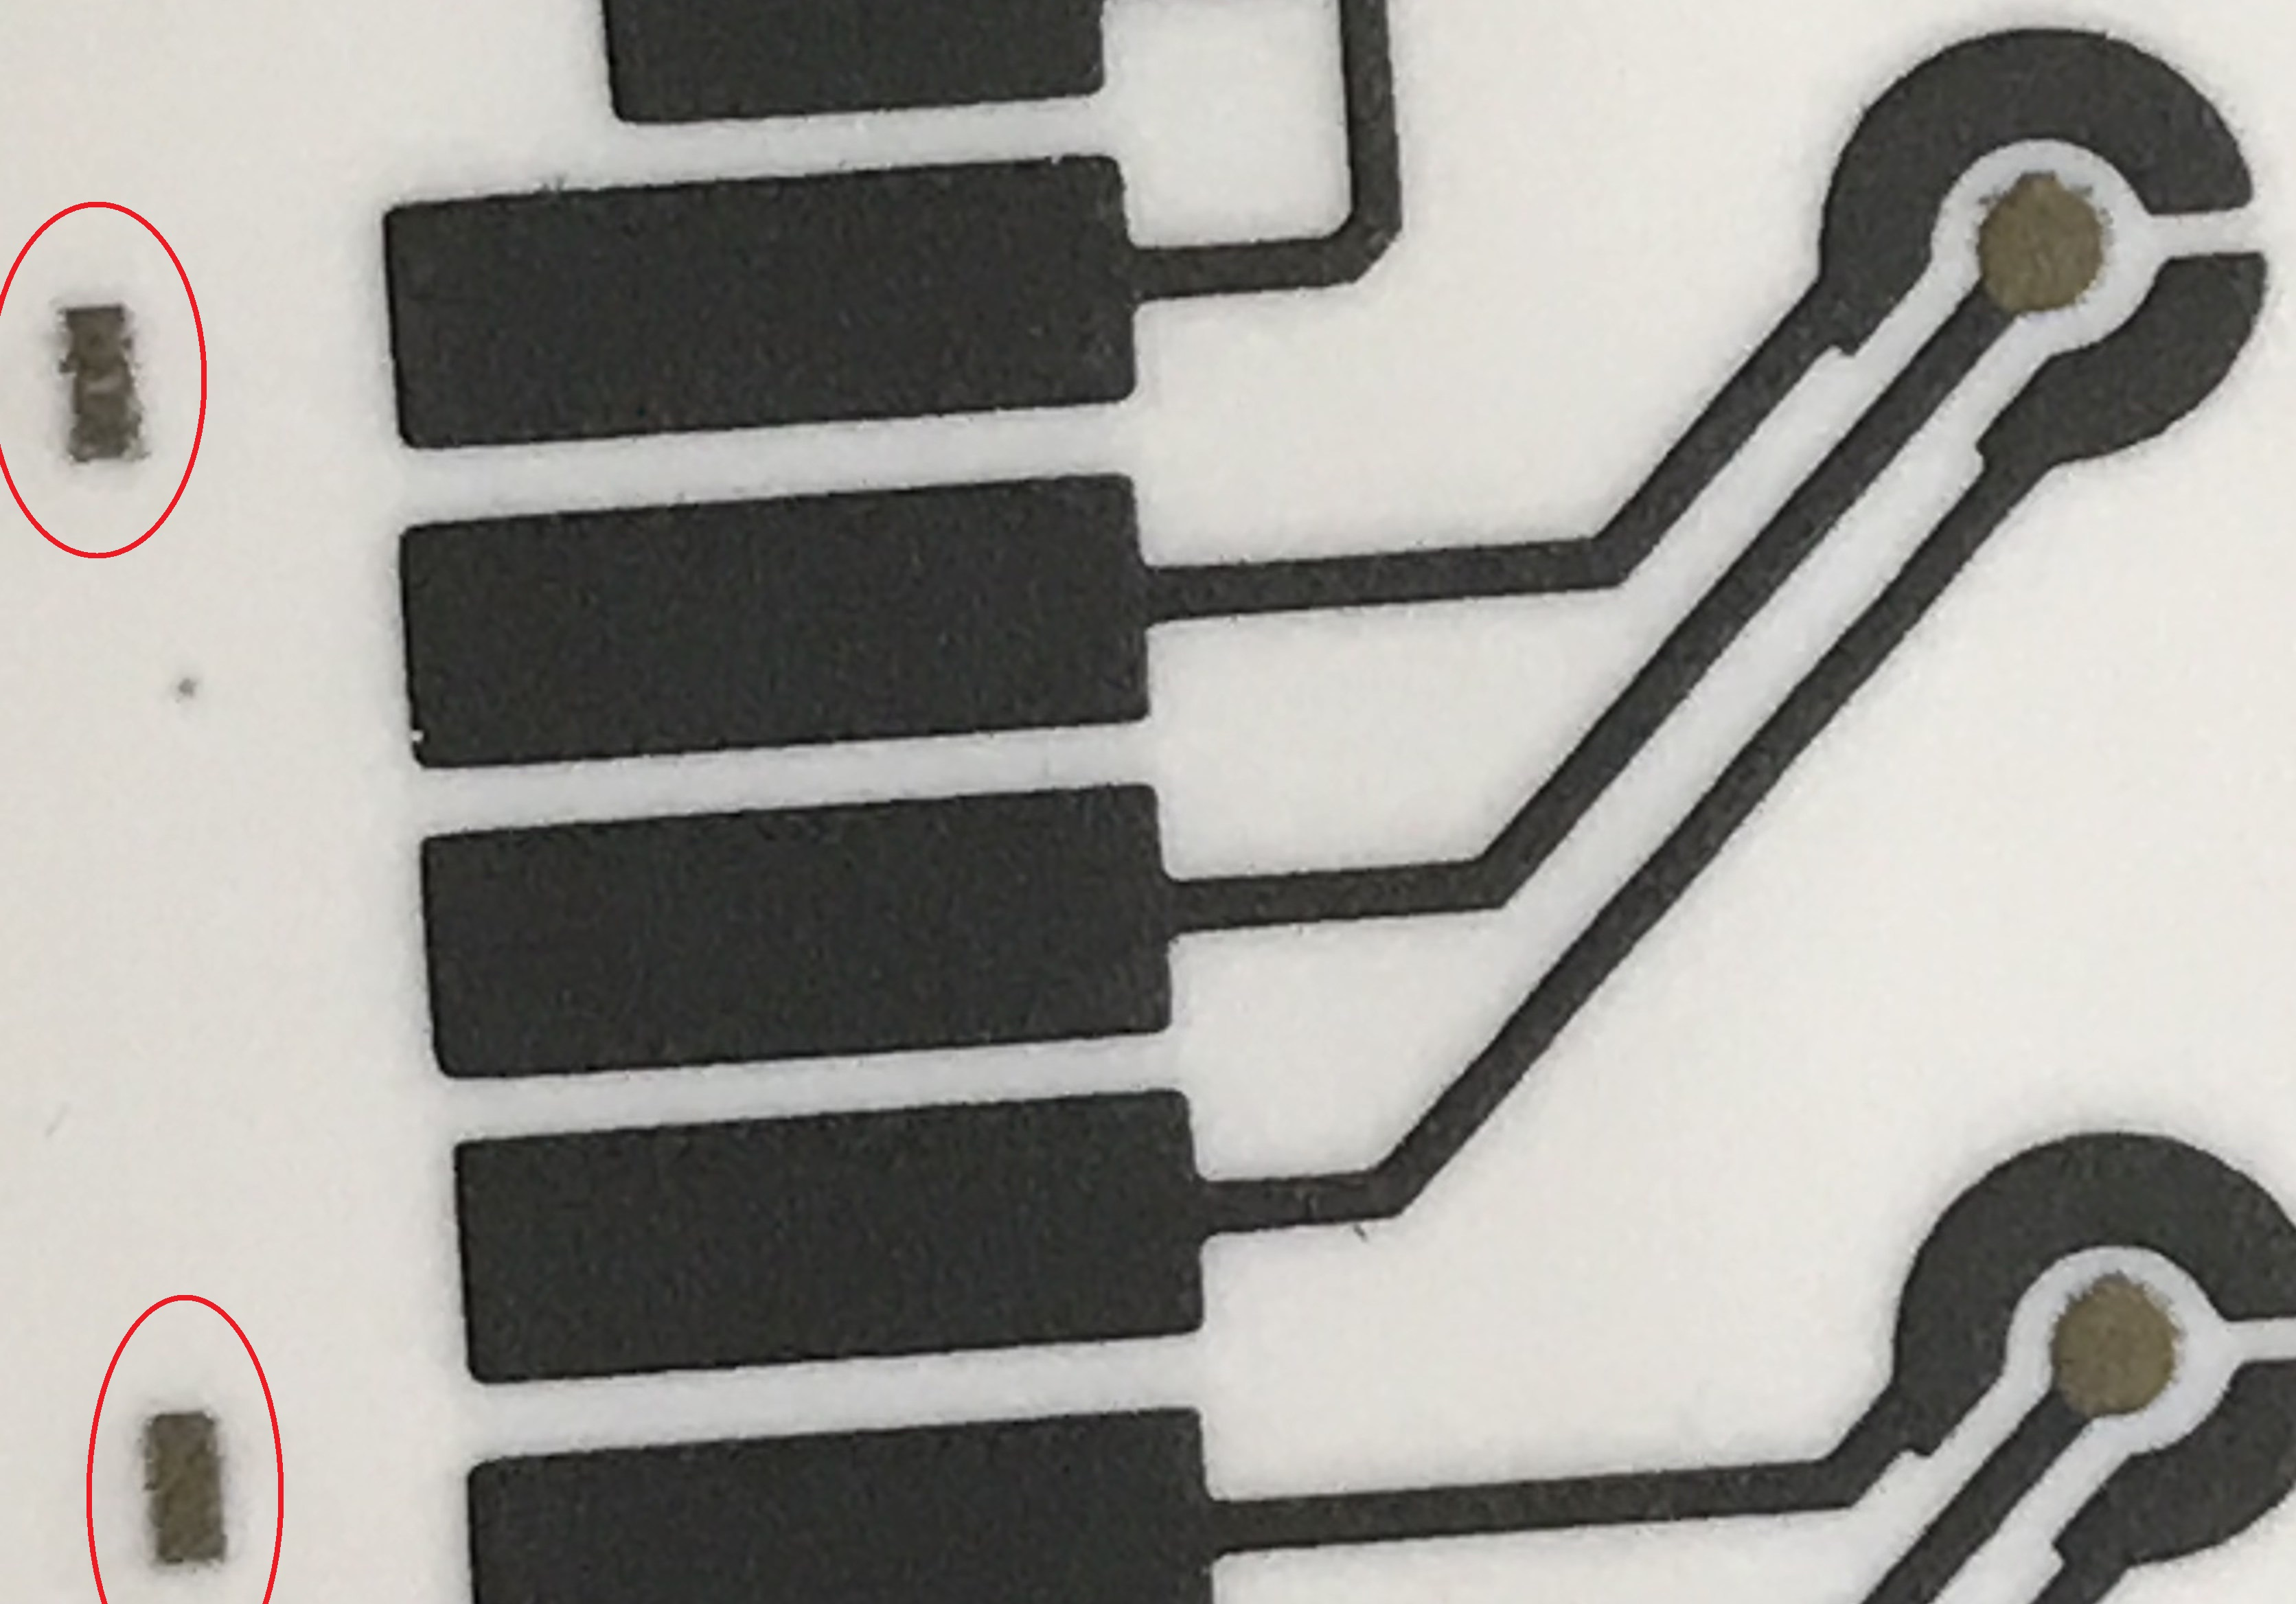
\includegraphics[width=0.5\textwidth]{Figures/Figura_Leader_Bar}
  \caption{$``$\textit{Leader Bars}$"$ printed on substrate.}
  \label{fig:Figura_Leader_Bar}
\end{figure}

At this point, if it was not done previously, it is advisable to calibrate the ejection voltages of the Nozzles that will be used by means of the $``$\textit{Drop Watcher}$"$ (Figure ~\ref{fig:Figura_nozzles}). This system consists of a camera oriented at 45º from the horizontal plane with focus on the Nozzles of the head that, by means of a strobe light, allows to photograph or film the operation of the holes in the head (Drop ejection).

\begin{figure}[H]
  \centering
    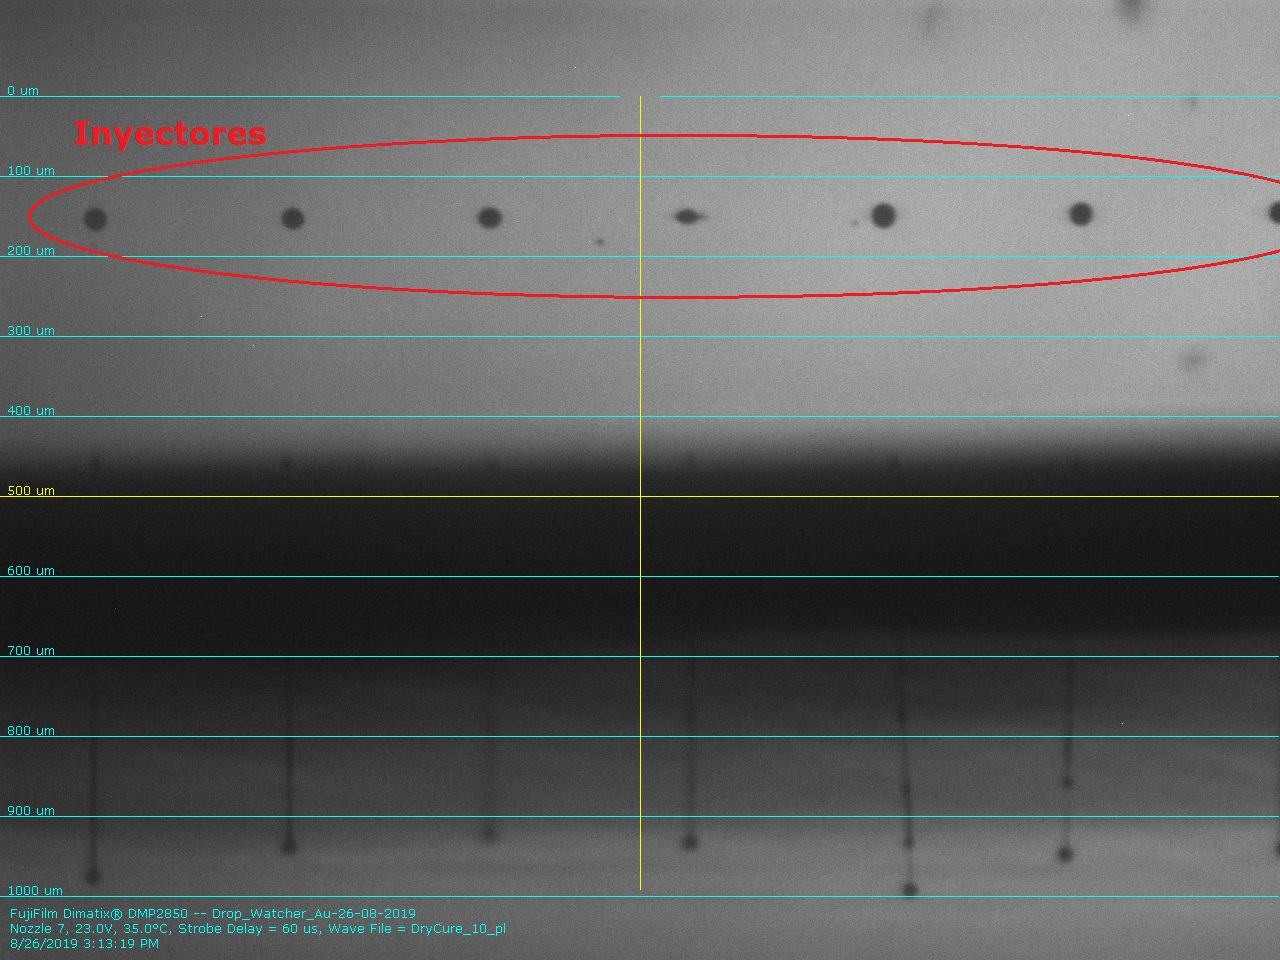
\includegraphics[width=0.5\textwidth]{Figures/Figura_nozzles}
  \caption{Nozzles seen from the $``$\textit{Drop Watcher}$"$ camera.}
  \label{fig:Figura_nozzles}
\end{figure}

Then, using the fiducial camera, the drops and substrate alignment processes are carried out and the coordinates where the printing begins are set.

Alignment of the substrate is accomplished by \textit{Theta} calibration. For this procedure, two points must be selected that are aligned on the substrate. In this case, the carbon print includes different alignment points. The smallest ones will be used to obtain greater precision, and thus minimizing the error due to the minimum width of the screen printing manufacturing (Figure ~\ref{fig:Figura_alineacion_theta}).

\begin{figure}[H]
  \centering
    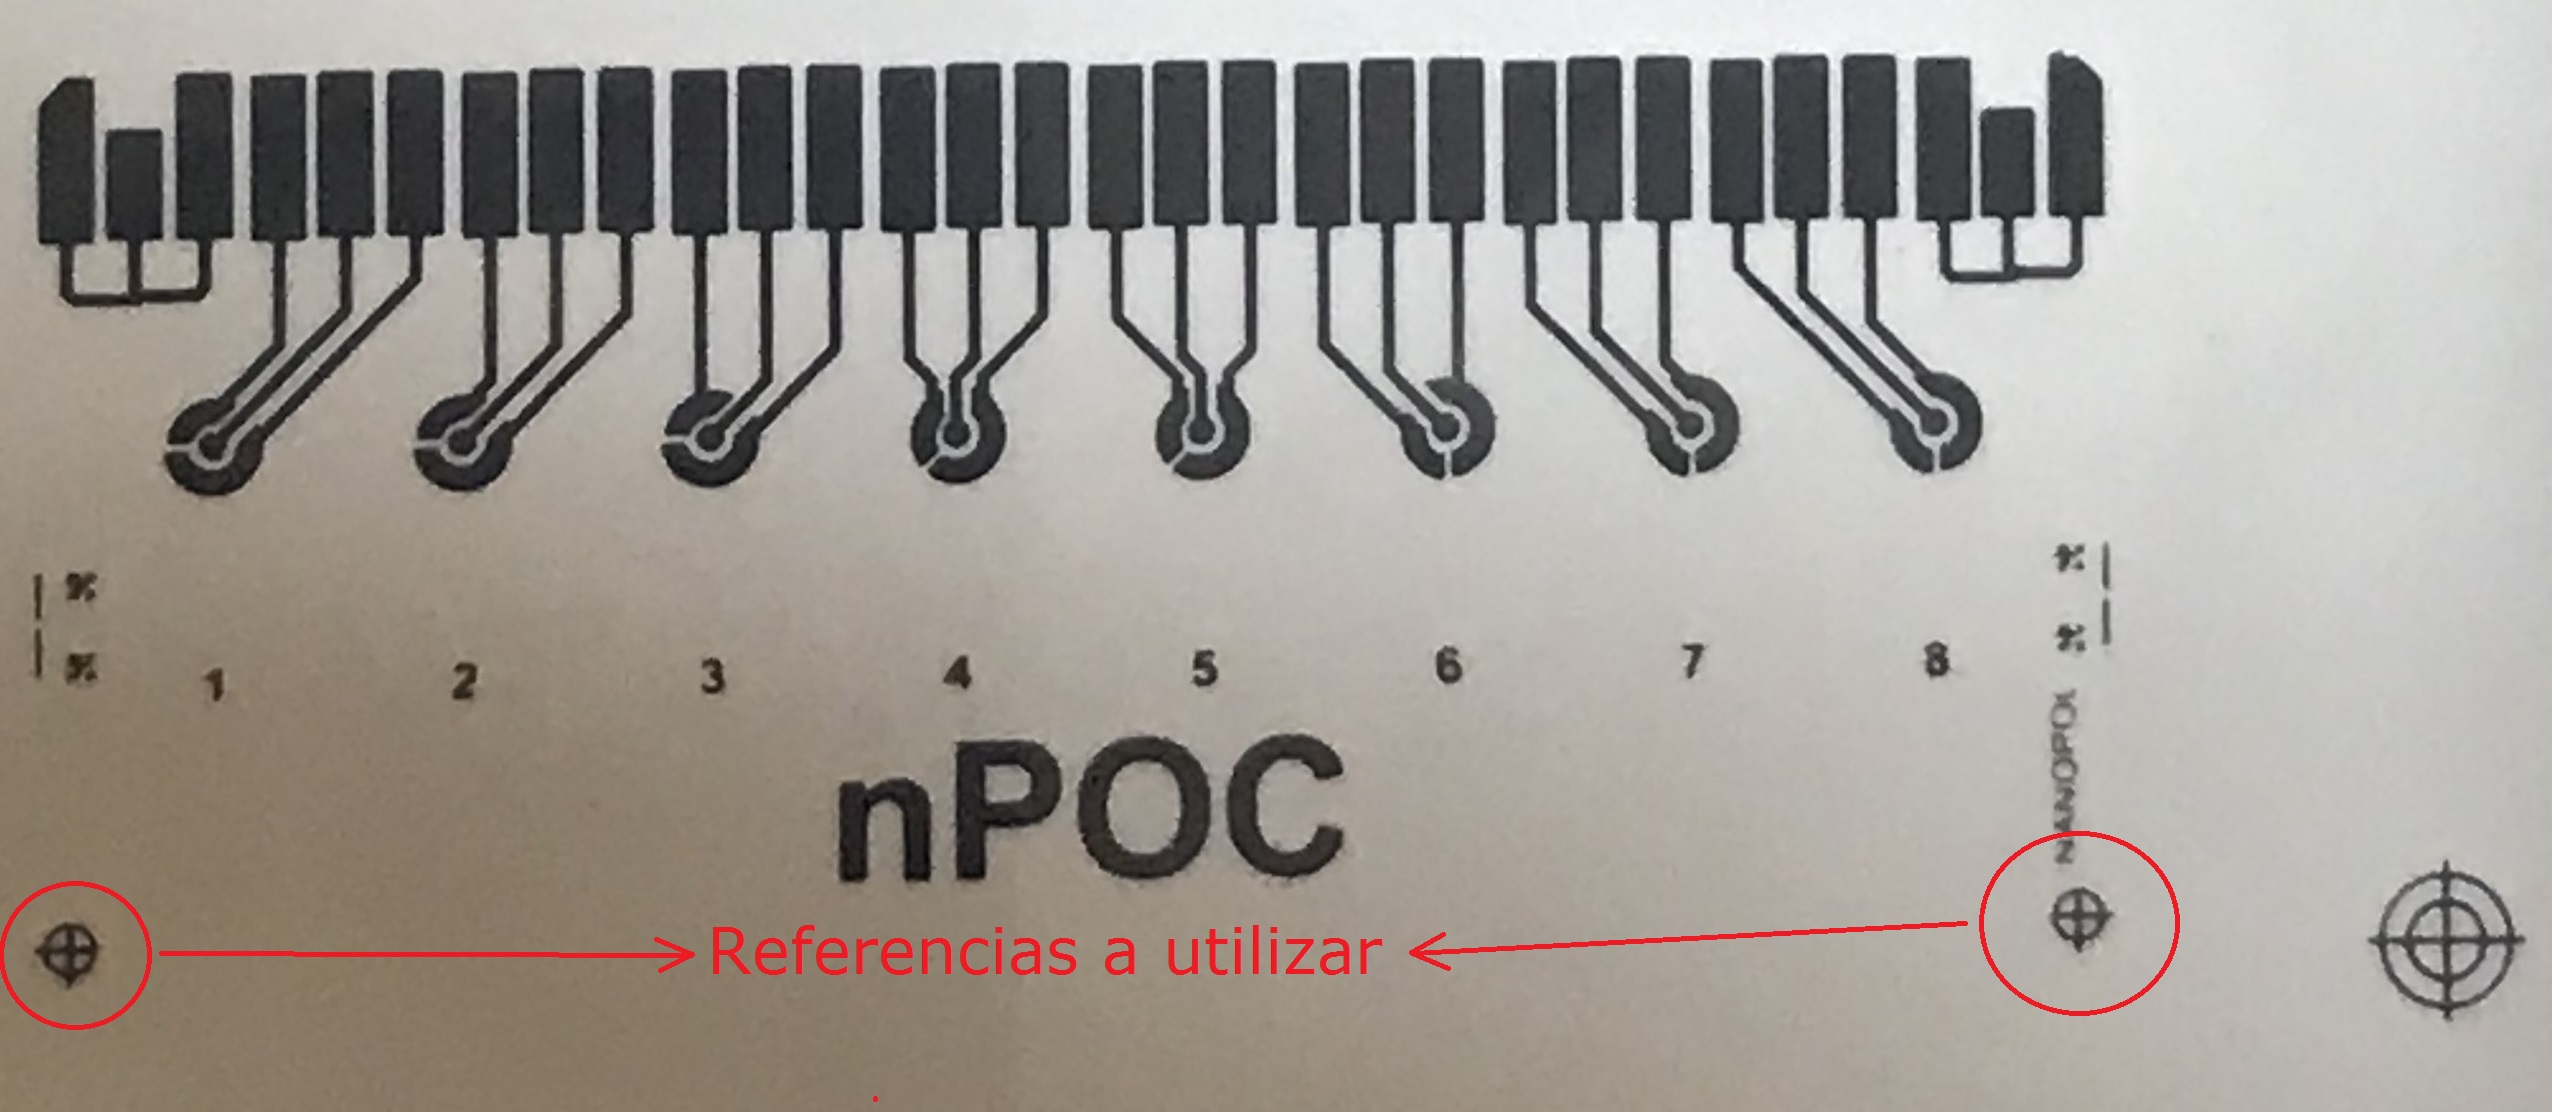
\includegraphics[width=0.5\textwidth]{Figures/Figura_alineacion_theta}
  \caption{References used for the \textit{Theta} calibration.}
  \label{fig:Figura_alineacion_theta}
\end{figure}

Although the alignment objects appear to be fine and regular to the naked eye, when using the fiducial camera it is observed that it is not easy to determine the midpoint (Figure ~\ref{fig:Figura_alineacion_theta2}).

\begin{figure}[H]
  \centering
    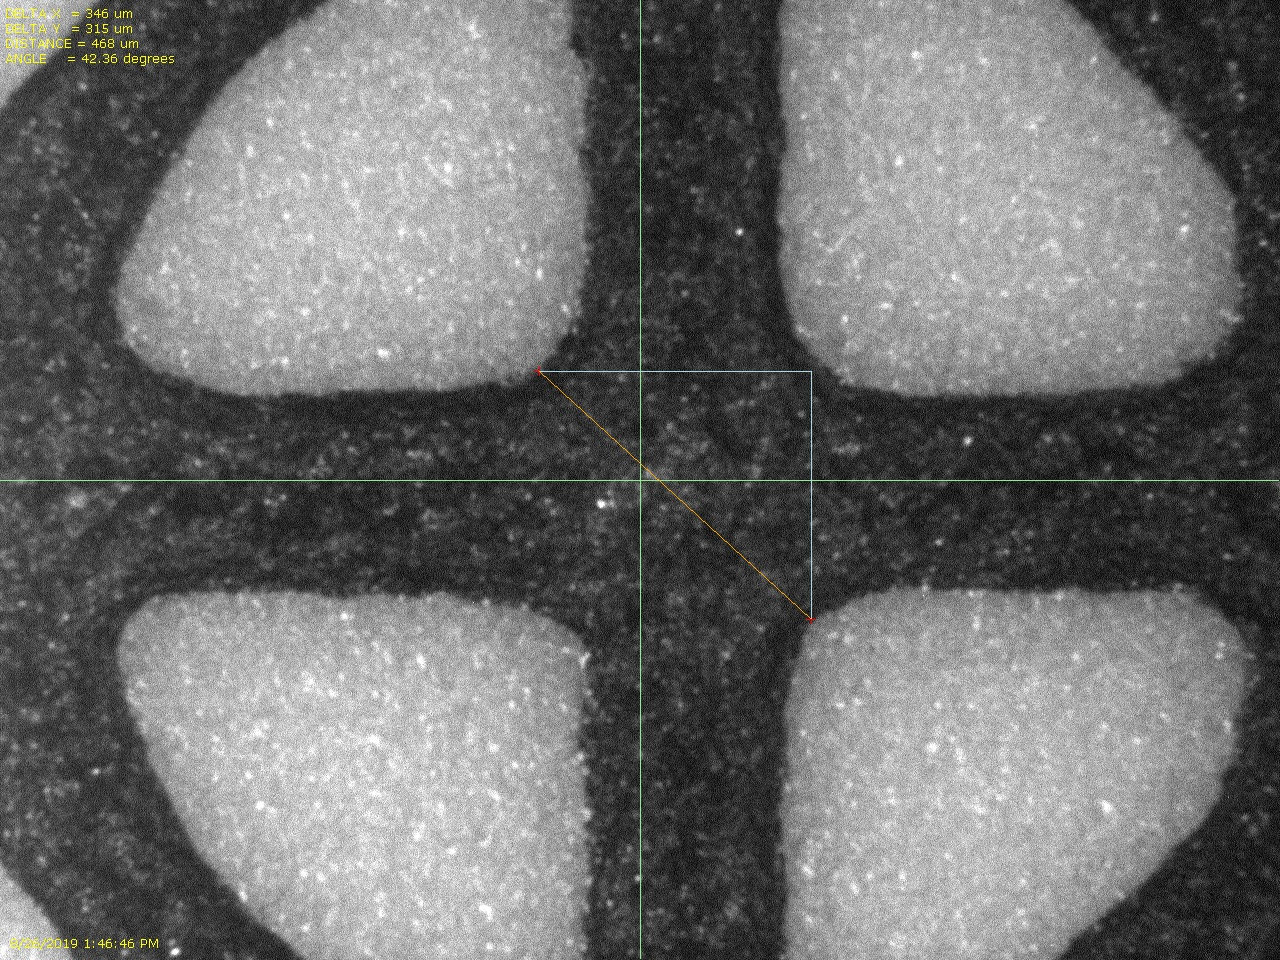
\includegraphics[width=0.4\textwidth]{Figures/Figura_alineacion_theta2}
  \caption{Alignment object seen with fiducial camera.}
  \label{fig:Figura_alineacion_theta2}
\end{figure}

Following the alignment of the substrate, it must be defined the spacing between drops that will be used when printing. This parameter is identified as $``$\textit{Drop Spacing}$"$ (from now on \emph{DS}) and, to determine it, a drop pattern with the different spacings allowed by the printer, called $``$\textit{Line Pattern}$"$, was used (Figure ~\ref{fig:Figura_Line_Pattern_Micro50X}). After printing, it is decided wich \emph{DS} generates the best defined line, both in continuity and in homogeneity of width and thickness, on the substrate to be used. For the gold ink on \textit{Valox} it was decided to use a spacing of 15 $\mu$m between drops, since it shows a continuous line without generating ink $``$\textit{Clusters}$"$.

\begin{figure}[H]
  \centering
    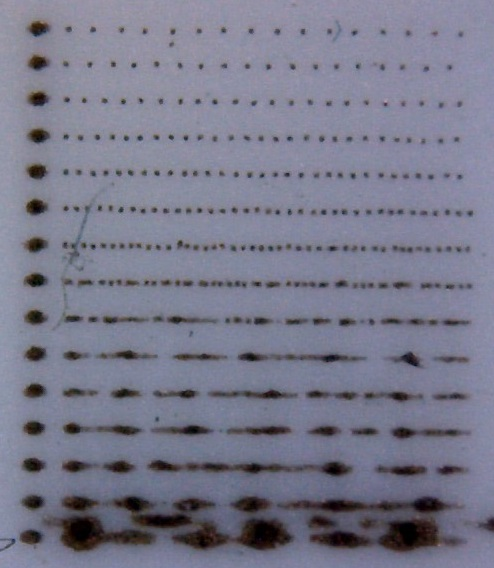
\includegraphics[width=0.35\textwidth]{Figures/Figura_Line_Pattern_Micro50X}
  \caption{$``$\textit{Line Pattern}$"$ viewed under a 50X microscope.}
  \label{fig:Figura_Line_Pattern_Micro50X}
\end{figure}

Once the \emph{DS} is defined, the resolution of the design to be printed is adjusted. In the case of 15 $\mu$m $``$\textit{Drop Spacing}$"$ between drops, a resolution of 1693.33 dots per inch (from now on \emph{dpi}) is used. The printer's instruction manual \cite{DimatixUM} provides a table with the resolution that the design should have and the angle at which the cartridge should be configured for each \emph{DS} (Figure ~\ref{fig:Figura_Tabla_angulos}).

\begin{figure}[H]
  \centering
    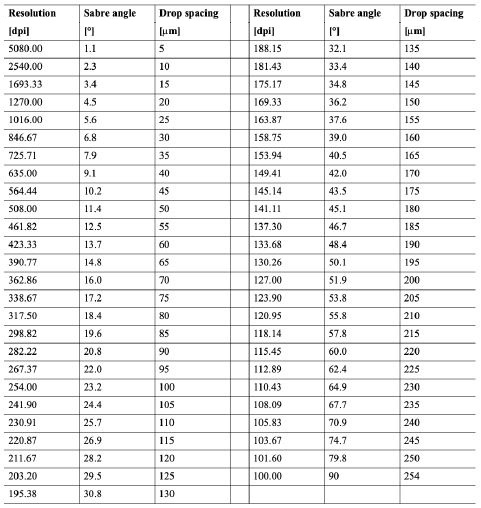
\includegraphics[width=0.5\textwidth]{Figures/Figura_Tabla_angulos}
  \caption{Table of resolutions and angles for each \emph{DS}.}
  \label{fig:Figura_Tabla_angulos}
\end{figure}

Next the $``$\textit{Drop Offset}$"$ calibration must be performed. This procedure compensates the error between the point where the fiducial camera is $``$looking$"$ and the position where the cartridge is printing. That is, it compensates the flight of the ink drops between its ejection from the head until it hits the substrate. For this, the printer makes a continuous line of 10 mm on the X axis followed by a point at 1 mm from the line. Calibration is performed once this point is located with the fiducial camera and $``$\textit{clicked}$"$ on it, as centered as possible (Figure ~\ref{fig:Figura_prueba_Drop_Spacing}).

\begin{figure}[H]
  \centering
    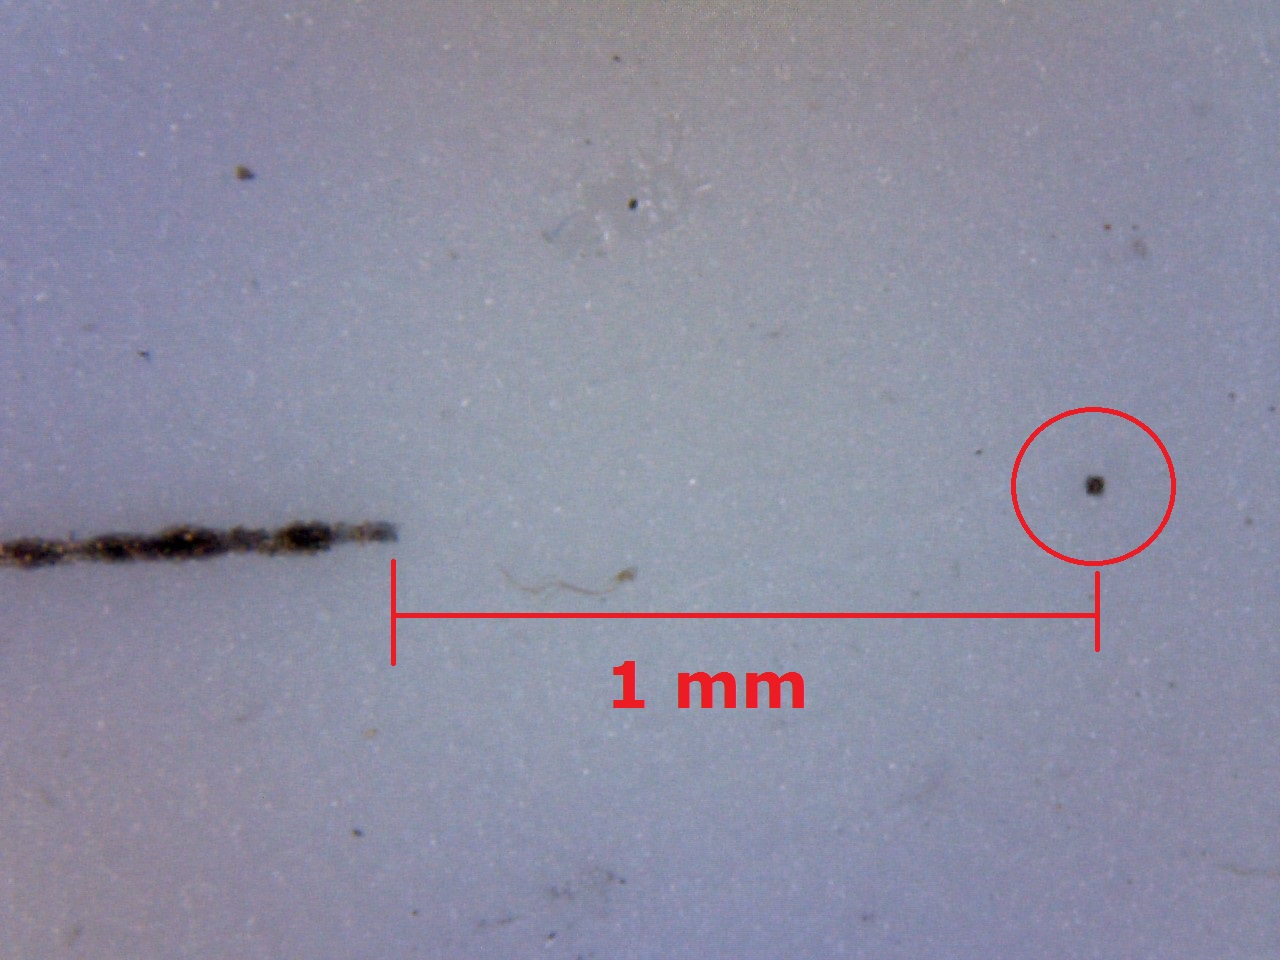
\includegraphics[width=0.5\textwidth]{Figures/Figura_prueba_Drop_Spacing}
  \caption{End of line and point of $``$\textit{Drop Offset}$"$ procedure, seen with a 1000X microscope.}
  \label{fig:Figura_prueba_Drop_Spacing}
\end{figure}

The fiducial camera is an element of the reel where the cartridge is placed (Figure ~\ref{fig:Figura_Camara_Fiducial}). This is used for the alignment procedures of the substrate, the calibration of the flight time of the ejected drops, the checkup of the substrate and the impressions on it or measurements on the surface placed on the stage. It has a field of view of 1.62 mm wide and 1.22 mm high, with a resolution of 2.54 $\mu$m per pixel.

\begin{figure}[H]
  \centering
    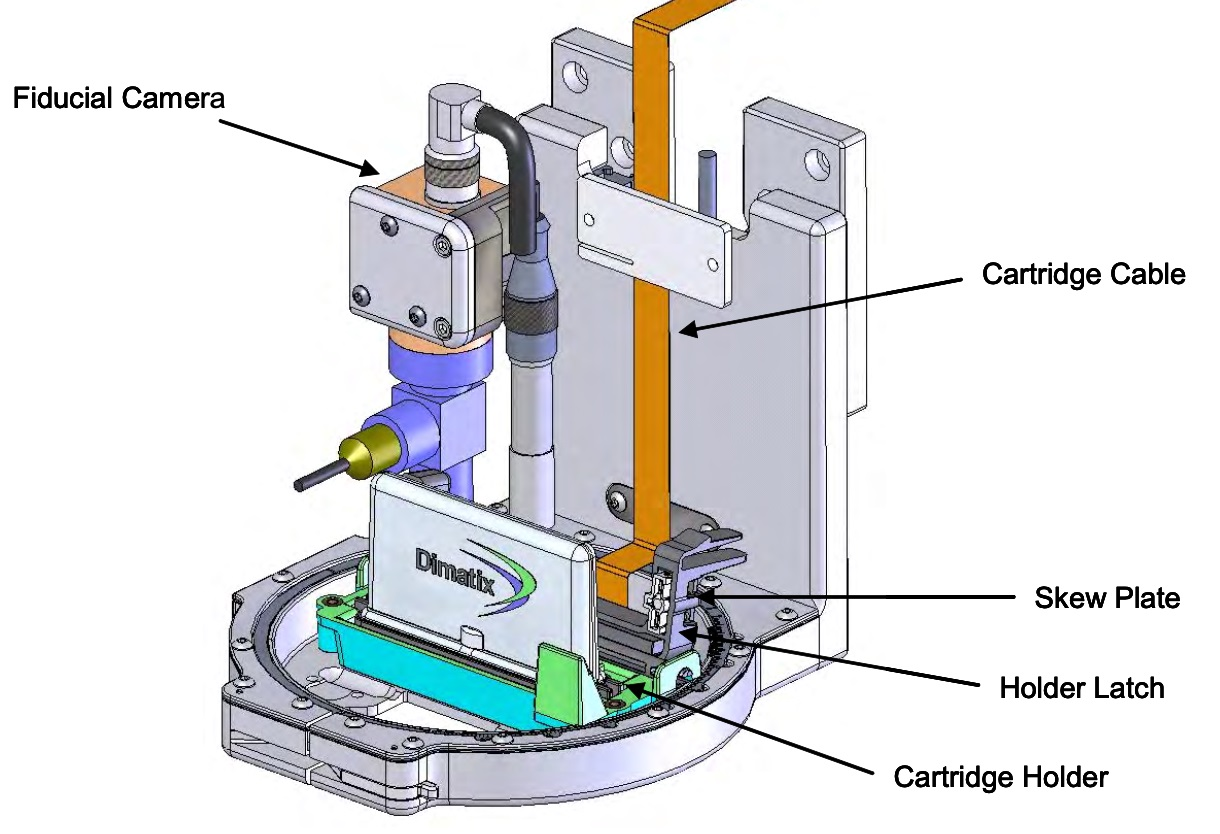
\includegraphics[width=0.5\textwidth]{Figures/Figura_Camara_Fiducial}
  \caption{Illustration of the different components of the printer reel.}
  \label{fig:Figura_Camara_Fiducial}
\end{figure}

As the last configuration before start printing, the coordinates of the substrate where it will start ($``$\textit{Print Origin}$"$) or a reference must be defined, which will agree with those defined in the design ($``$\textit{Reference Point}$"$).

If it is decided to use the point where it will start printing, \textit{Set Print Origin} function of the fiducial chamber must be chosen. On the other hand, if it will use a reference point of the design with the substrate, \textit{Set Reference Point} function must be configured (Figure ~\ref{fig:Figura_Ventana_Camara_Fiducial}). When using this last function, it must be taken into account that the reference point must be defined in the design before loading it in the image to print tab of the \textit{DMP} software.

\begin{figure}[H]
  \centering
    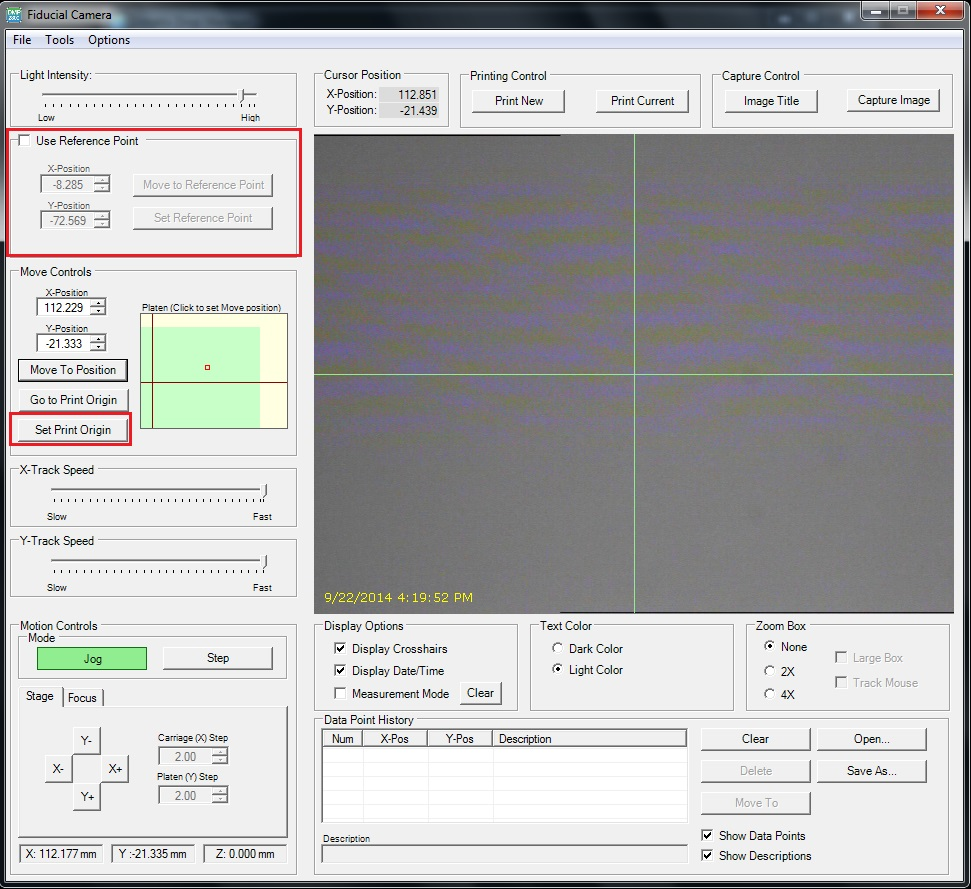
\includegraphics[width=0.5\textwidth]{Figures/Figura_Ventana_Camara_Fiducial}
  \caption{Fiducial camera window with options for \textit{Print Origin} and \textit{Reference Point}.}
  \label{fig:Figura_Ventana_Camara_Fiducial}
\end{figure}

For this work it was decided to use the center of the first circle as a reference point, aligning it with the working electrode 1 of the sensor. In this way, the other 7 circles were aligned with their respective electrode.

\section{Prints}
As a first test, a 1 mm diameter circle was printed on the carbon ink and on the \textit{Valox} substrate, to verify the behavior of the gold ink on both surfaces (Figure ~\ref{fig:Figura_Prueba_Sobre_Sustratos}).

\begin{figure}[H]
  \centering
    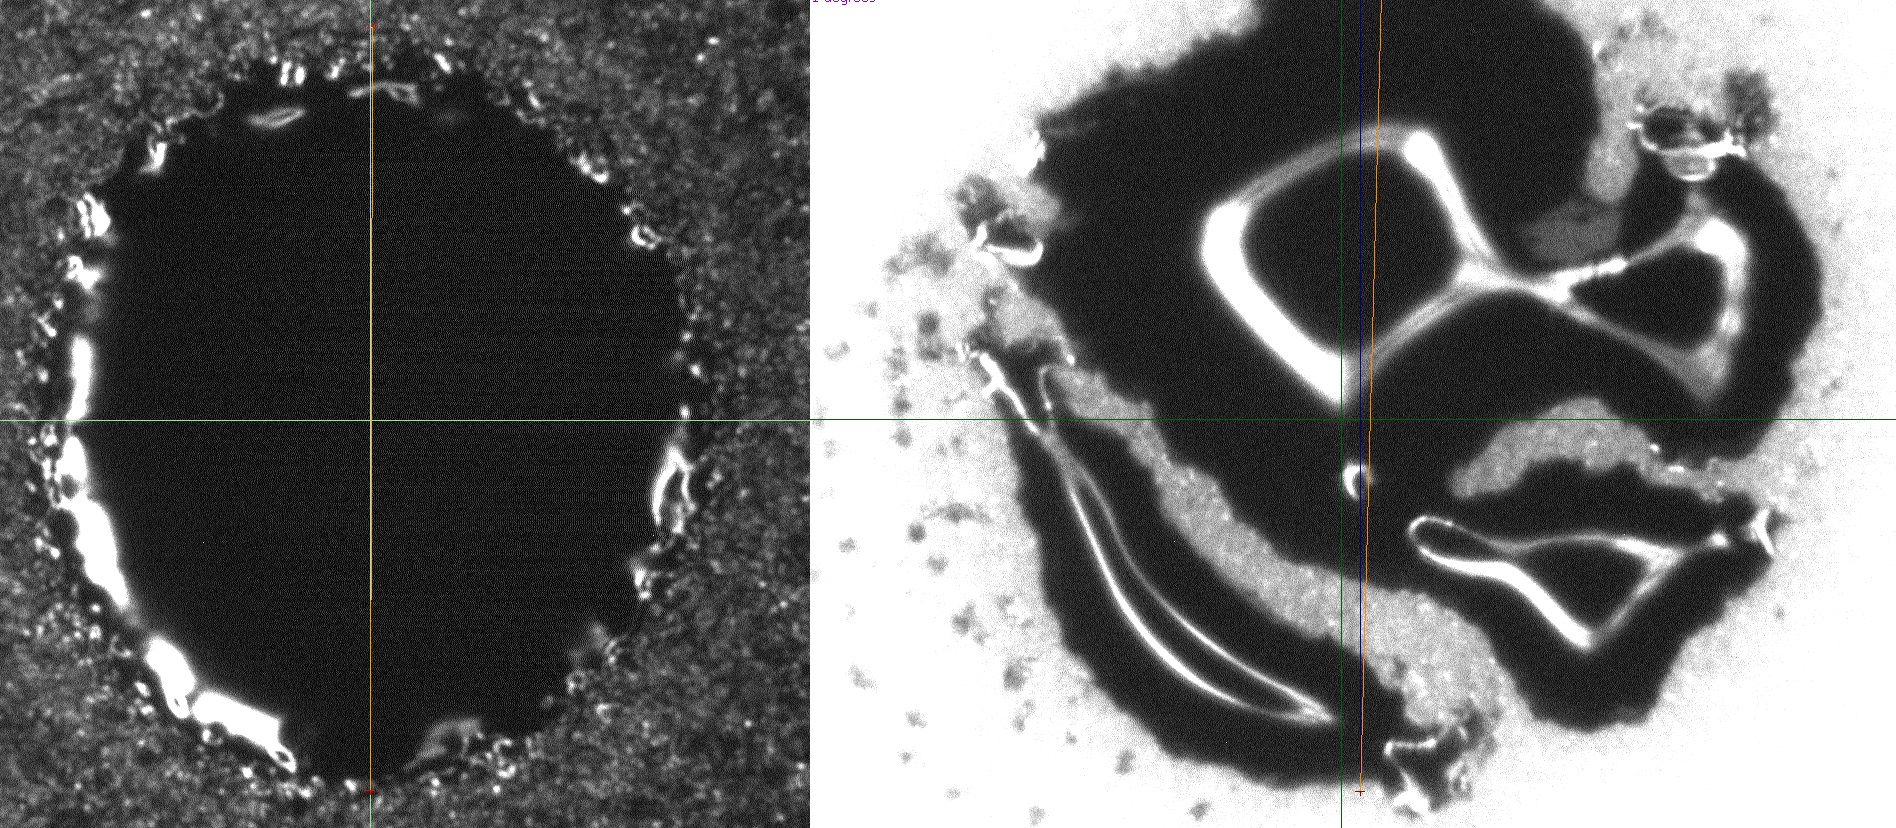
\includegraphics[width=0.5\textwidth]{Figures/Figura_Prueba_Sobre_Sustratos}
  \caption{Test of gold ink on carbon ink and \textit{Valox} substrate.}
  \label{fig:Figura_Prueba_Sobre_Sustratos}
\end{figure}

As expected, the gold ink shows better anchor on carbon than on the substrate.

The next test was to align the reference point with the drawing to be printed in the center of the first working electrode (WE1) of the biosensor called \textit{nPoc1}, make the printing of an ink layer and take the time it takes for the ink to be absorbed (Figure ~\ref{fig:Figura_Primera_impresion_circulo}). To obtain an average of the necessary time, the same printing procedure is repeated on the eight electrodes of the \textit{nPoc1}.

\begin{figure}[H]
  \centering
    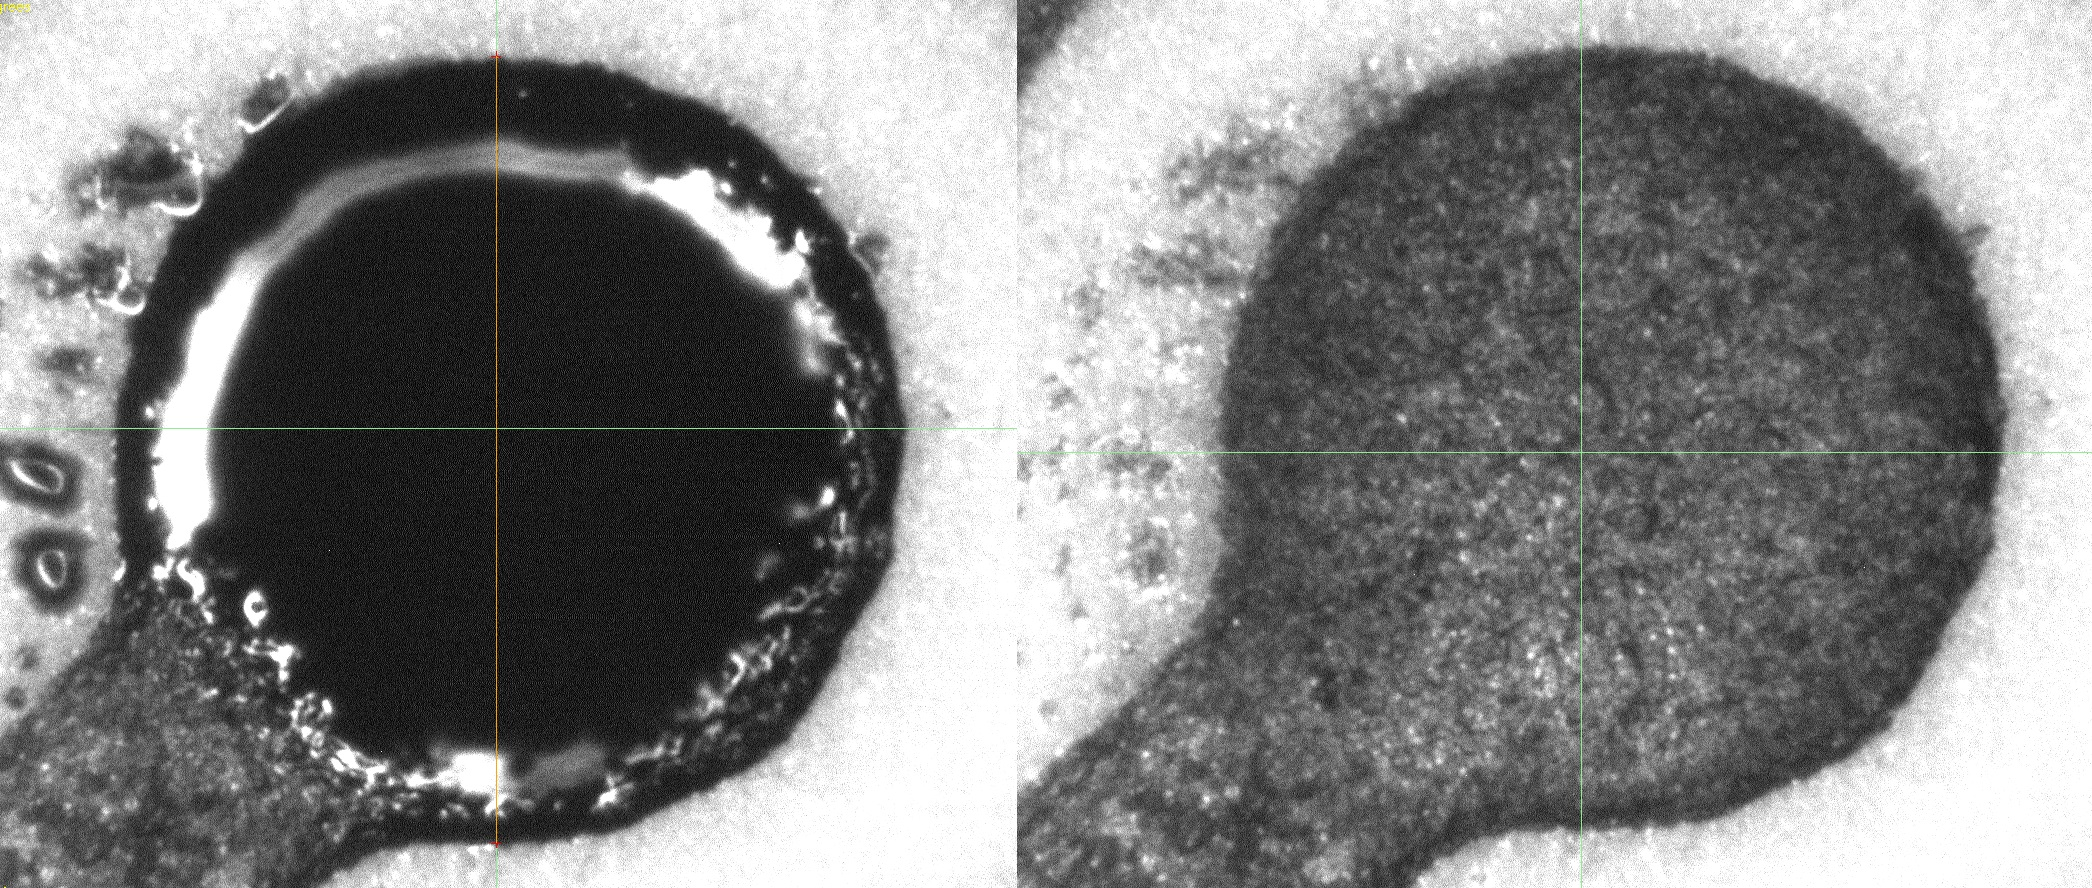
\includegraphics[width=0.5\textwidth]{Figures/Figura_Primera_impresion_circulo}
  \caption{First impression on working electrode (WE1).}
  \label{fig:Figura_Primera_impresion_circulo}
\end{figure}

It is concluded that the average time necessary for drying the ink is 10 minutes. The ink will not be completely dry and anchored until it is cured. For the gold ink curing procedure on \textit{Valox} substrate, a \textit{Hot Plate} is used at 80ºC for 80 minutes (Figure ~\ref{fig:Figura_Hot_Plate}).

\begin{figure}[H]
  \centering
    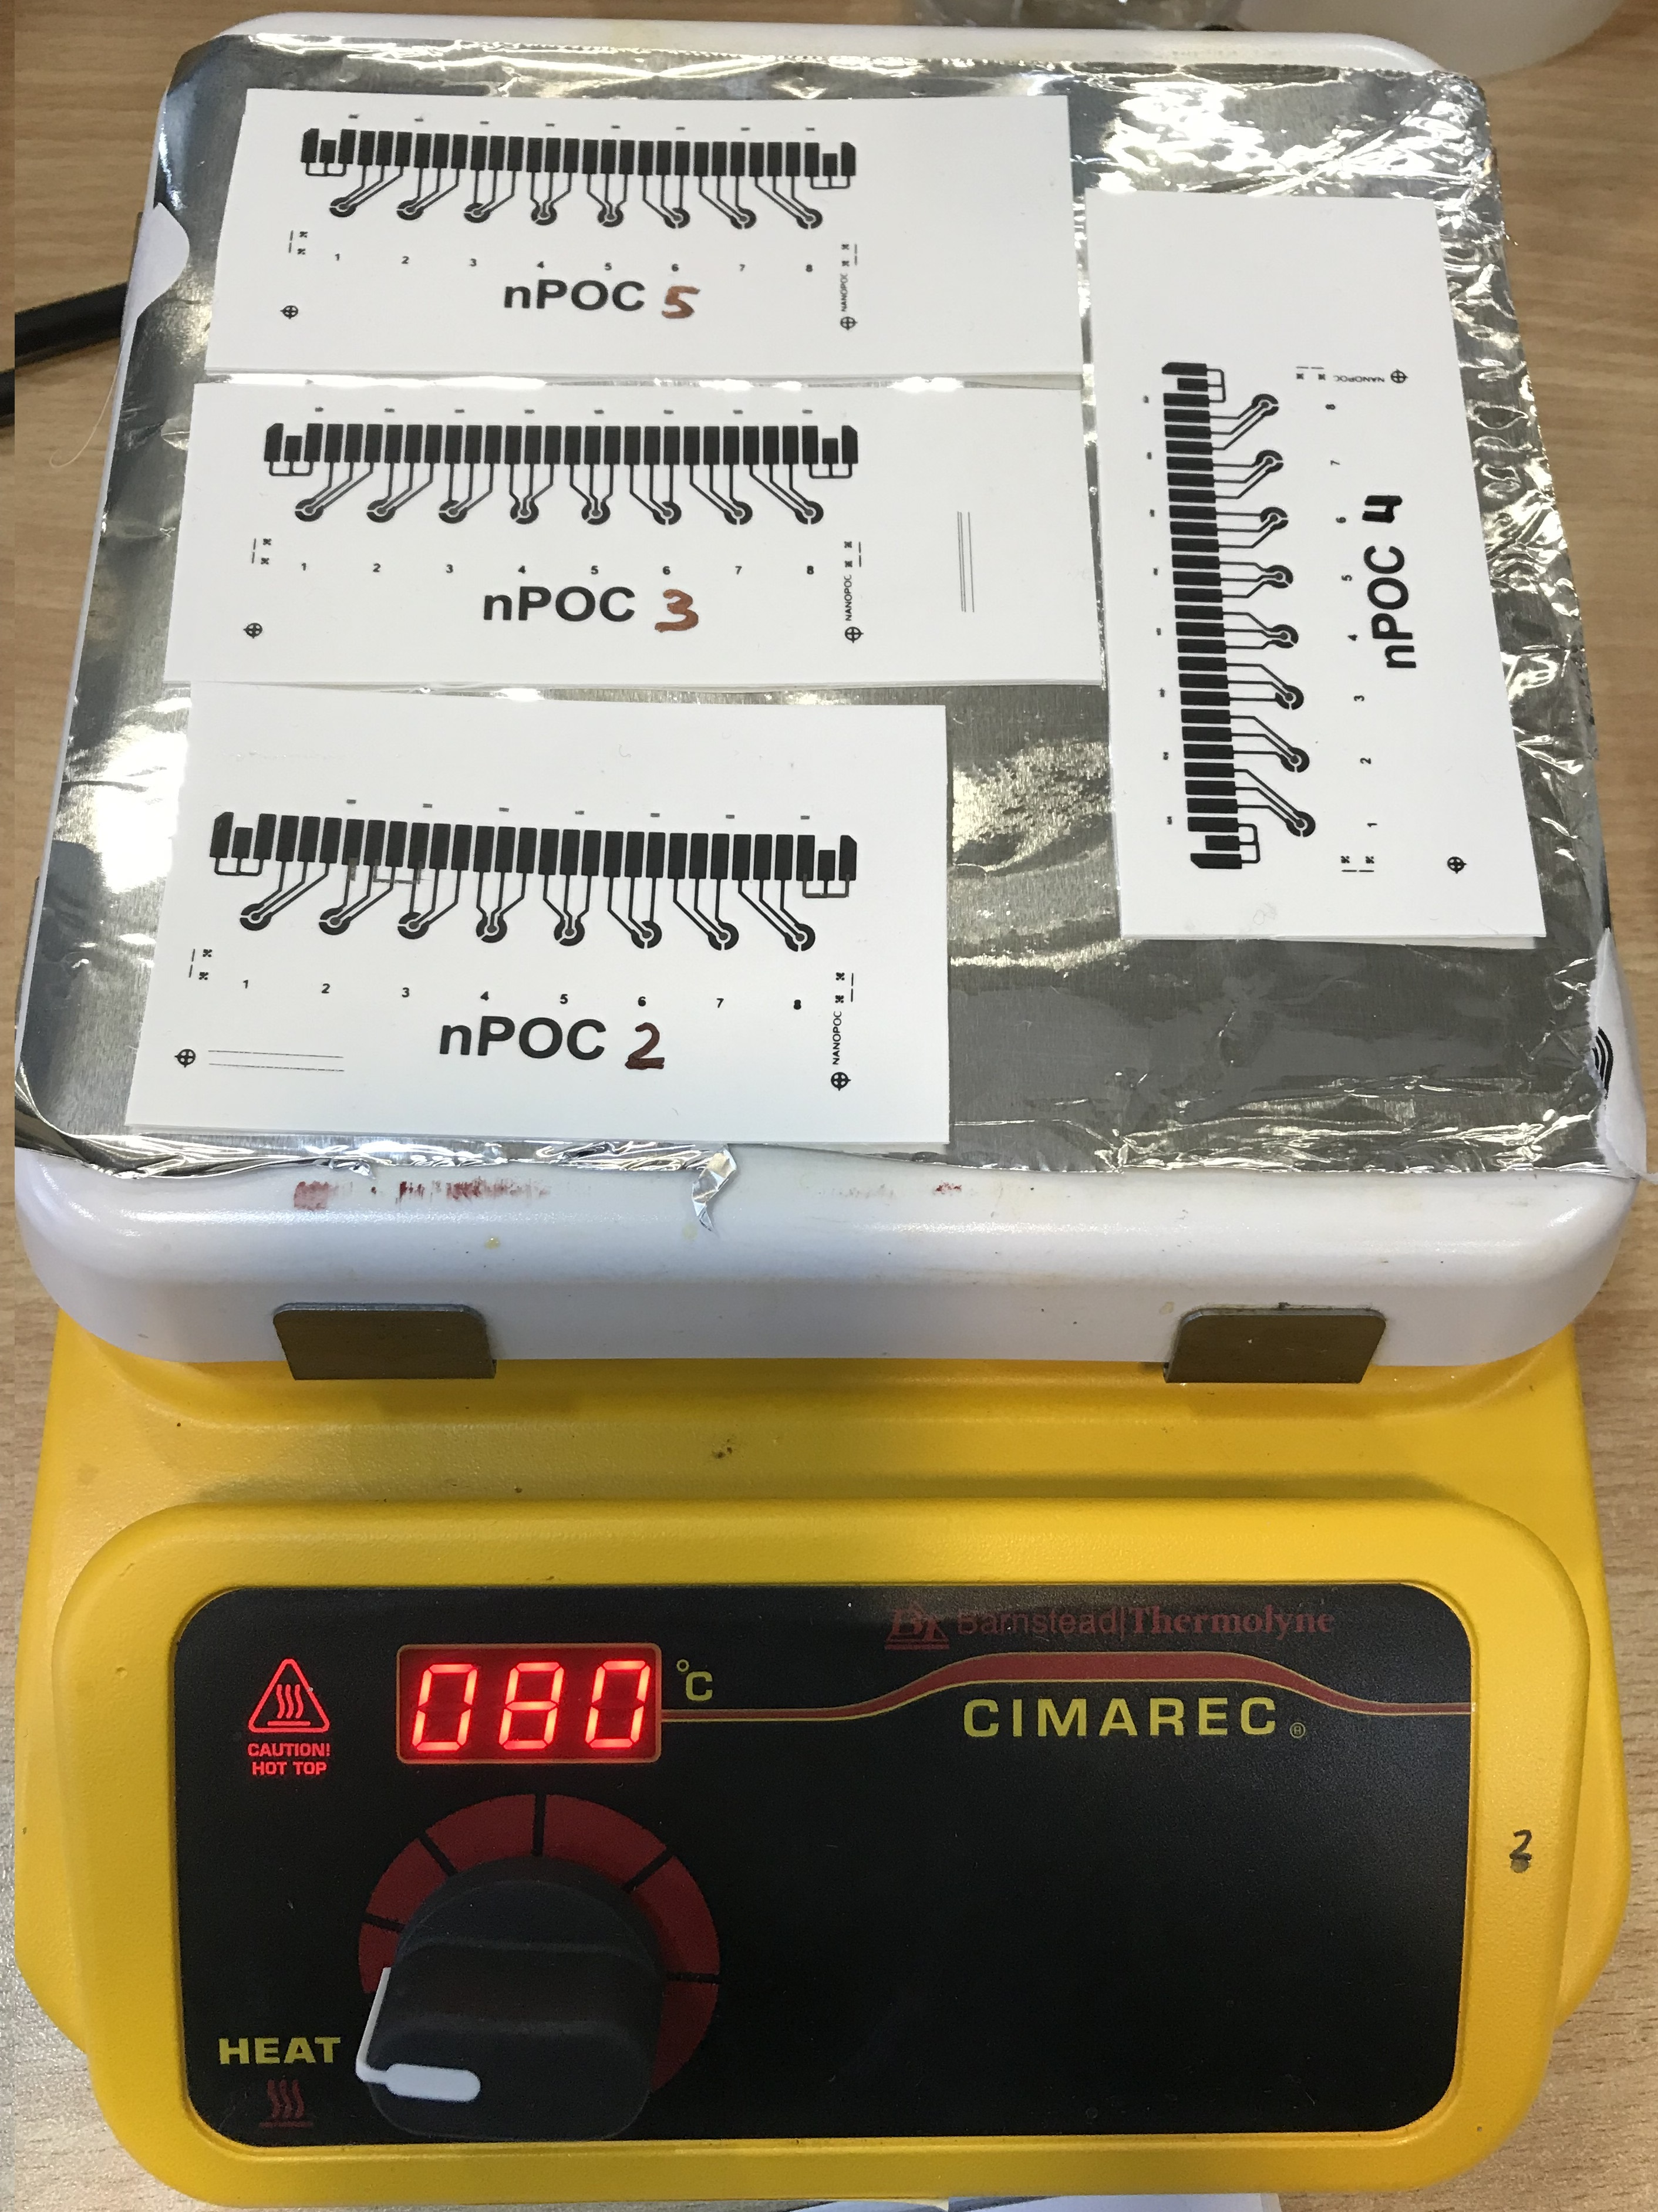
\includegraphics[width=0.4\textwidth]{Figures/Figura_Hot_Plate}
  \caption{\textit{Hot Plate} electrode curing.}
  \label{fig:Figura_Hot_Plate}
\end{figure}

The second printing is made with 1.1 mm diameter circles, to compare the results with the previous work. The 8 working electrodes of the \textit{nPoc5} are printed, one at a time. As can be seen (Figure ~\ref{fig:Figura_Segunda_Impresion_circulo}), the ink that falls on the substrate does not anchor correctly, generating \textit{clusters} of it outside the \emph{WE}.

\begin{figure}[H]
  \centering
    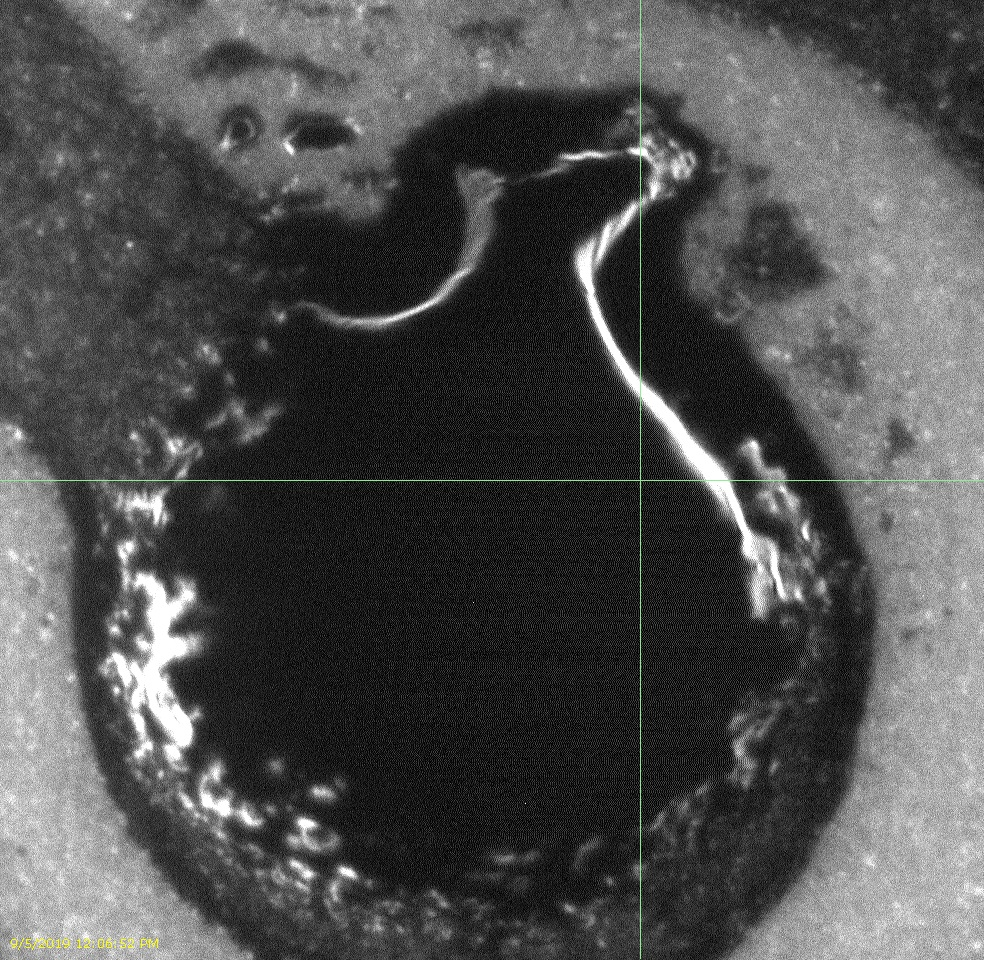
\includegraphics[width=0.45\textwidth]{Figures/Figura_Segunda_Impresion_circulo}
  \caption{1.1 mm circle print on \emph{WE}.}
  \label{fig:Figura_Segunda_Impresion_circulo}
\end{figure}

To increase the level of reproducibility on a larger scale, a pattern of eight circles of 1 mm diameter each is designed. The reference point is centered on the first circle and aligned with the center of the first \emph{WE} of the \textit{nPoc3} substrate.

Slight deviations are noted in the deposition of the gold ink, this may be due to the variations obtained by the screen printing of the carbon ink pattern. However, no significant ink spills are detected on the \textit{Valox} substrate (Figure ~\ref{fig:Figura_impresion_8juntos}).

\begin{figure}[H]
  \centering
    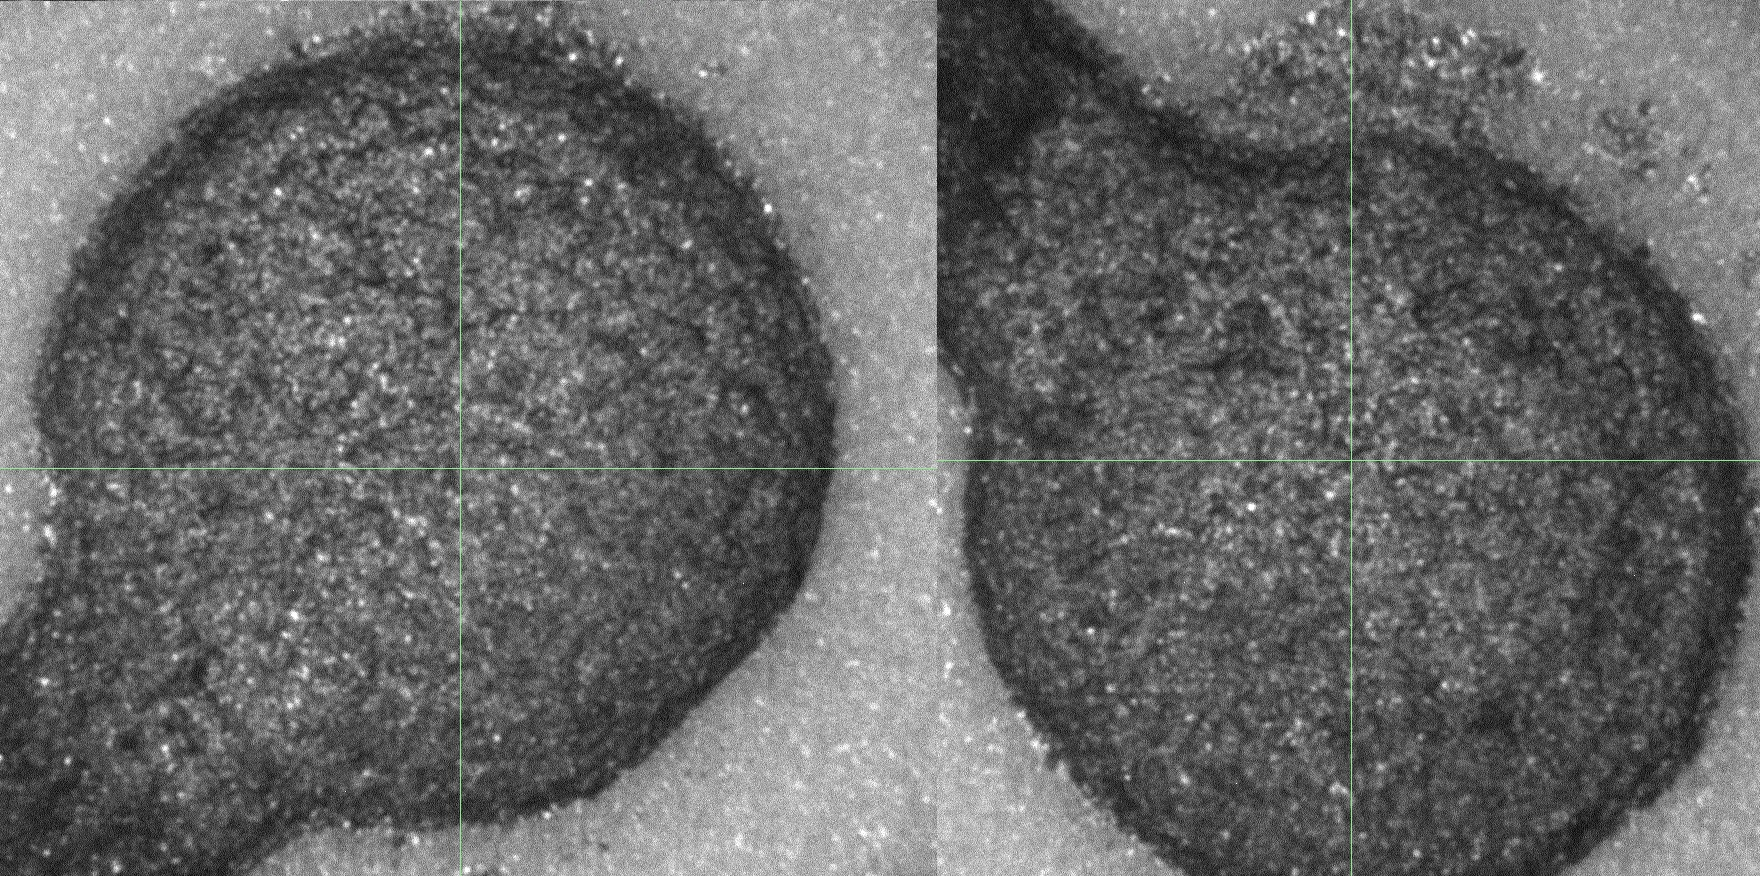
\includegraphics[width=0.6\textwidth]{Figures/Figura_impresion_8juntos}
  \caption{Print comparison between \emph{WE} 3 and 5.}
  \label{fig:Figura_impresion_8juntos}
\end{figure}

The biosensor is then cured on a \textit{Hot Plate} at 80ºC for 80 minutes. The ink is observed to take on a lighter color, similar to the color of pure gold (Figura ~\ref{fig:Figura_impresion_curado}).

\begin{figure}[H]
  \centering
    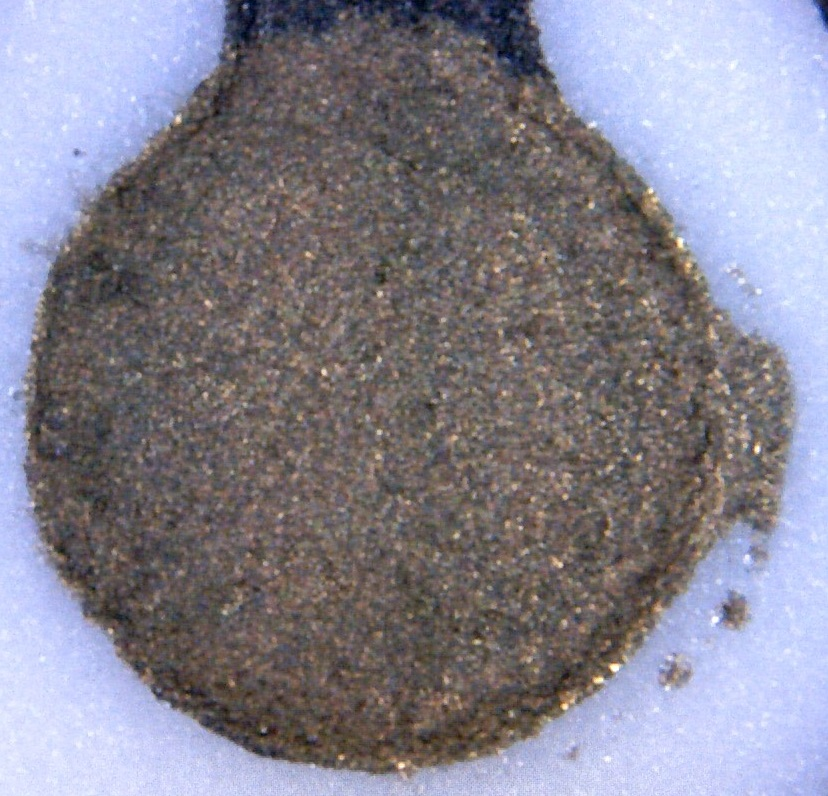
\includegraphics[width=0.45\textwidth]{Figures/Figura_impresion_curado}
  \caption{USB 1000X microscope image of \emph{WE} cured in \textit{Hot Plate}.}
  \label{fig:Figura_impresion_curado}
\end{figure}

For electrical characterization, a pattern was designed in the form of the connection between two test contacts of the biosensor (Figure ~\ref{fig:Figura_contactos_prueba}).

\begin{figure}[H]
  \centering
    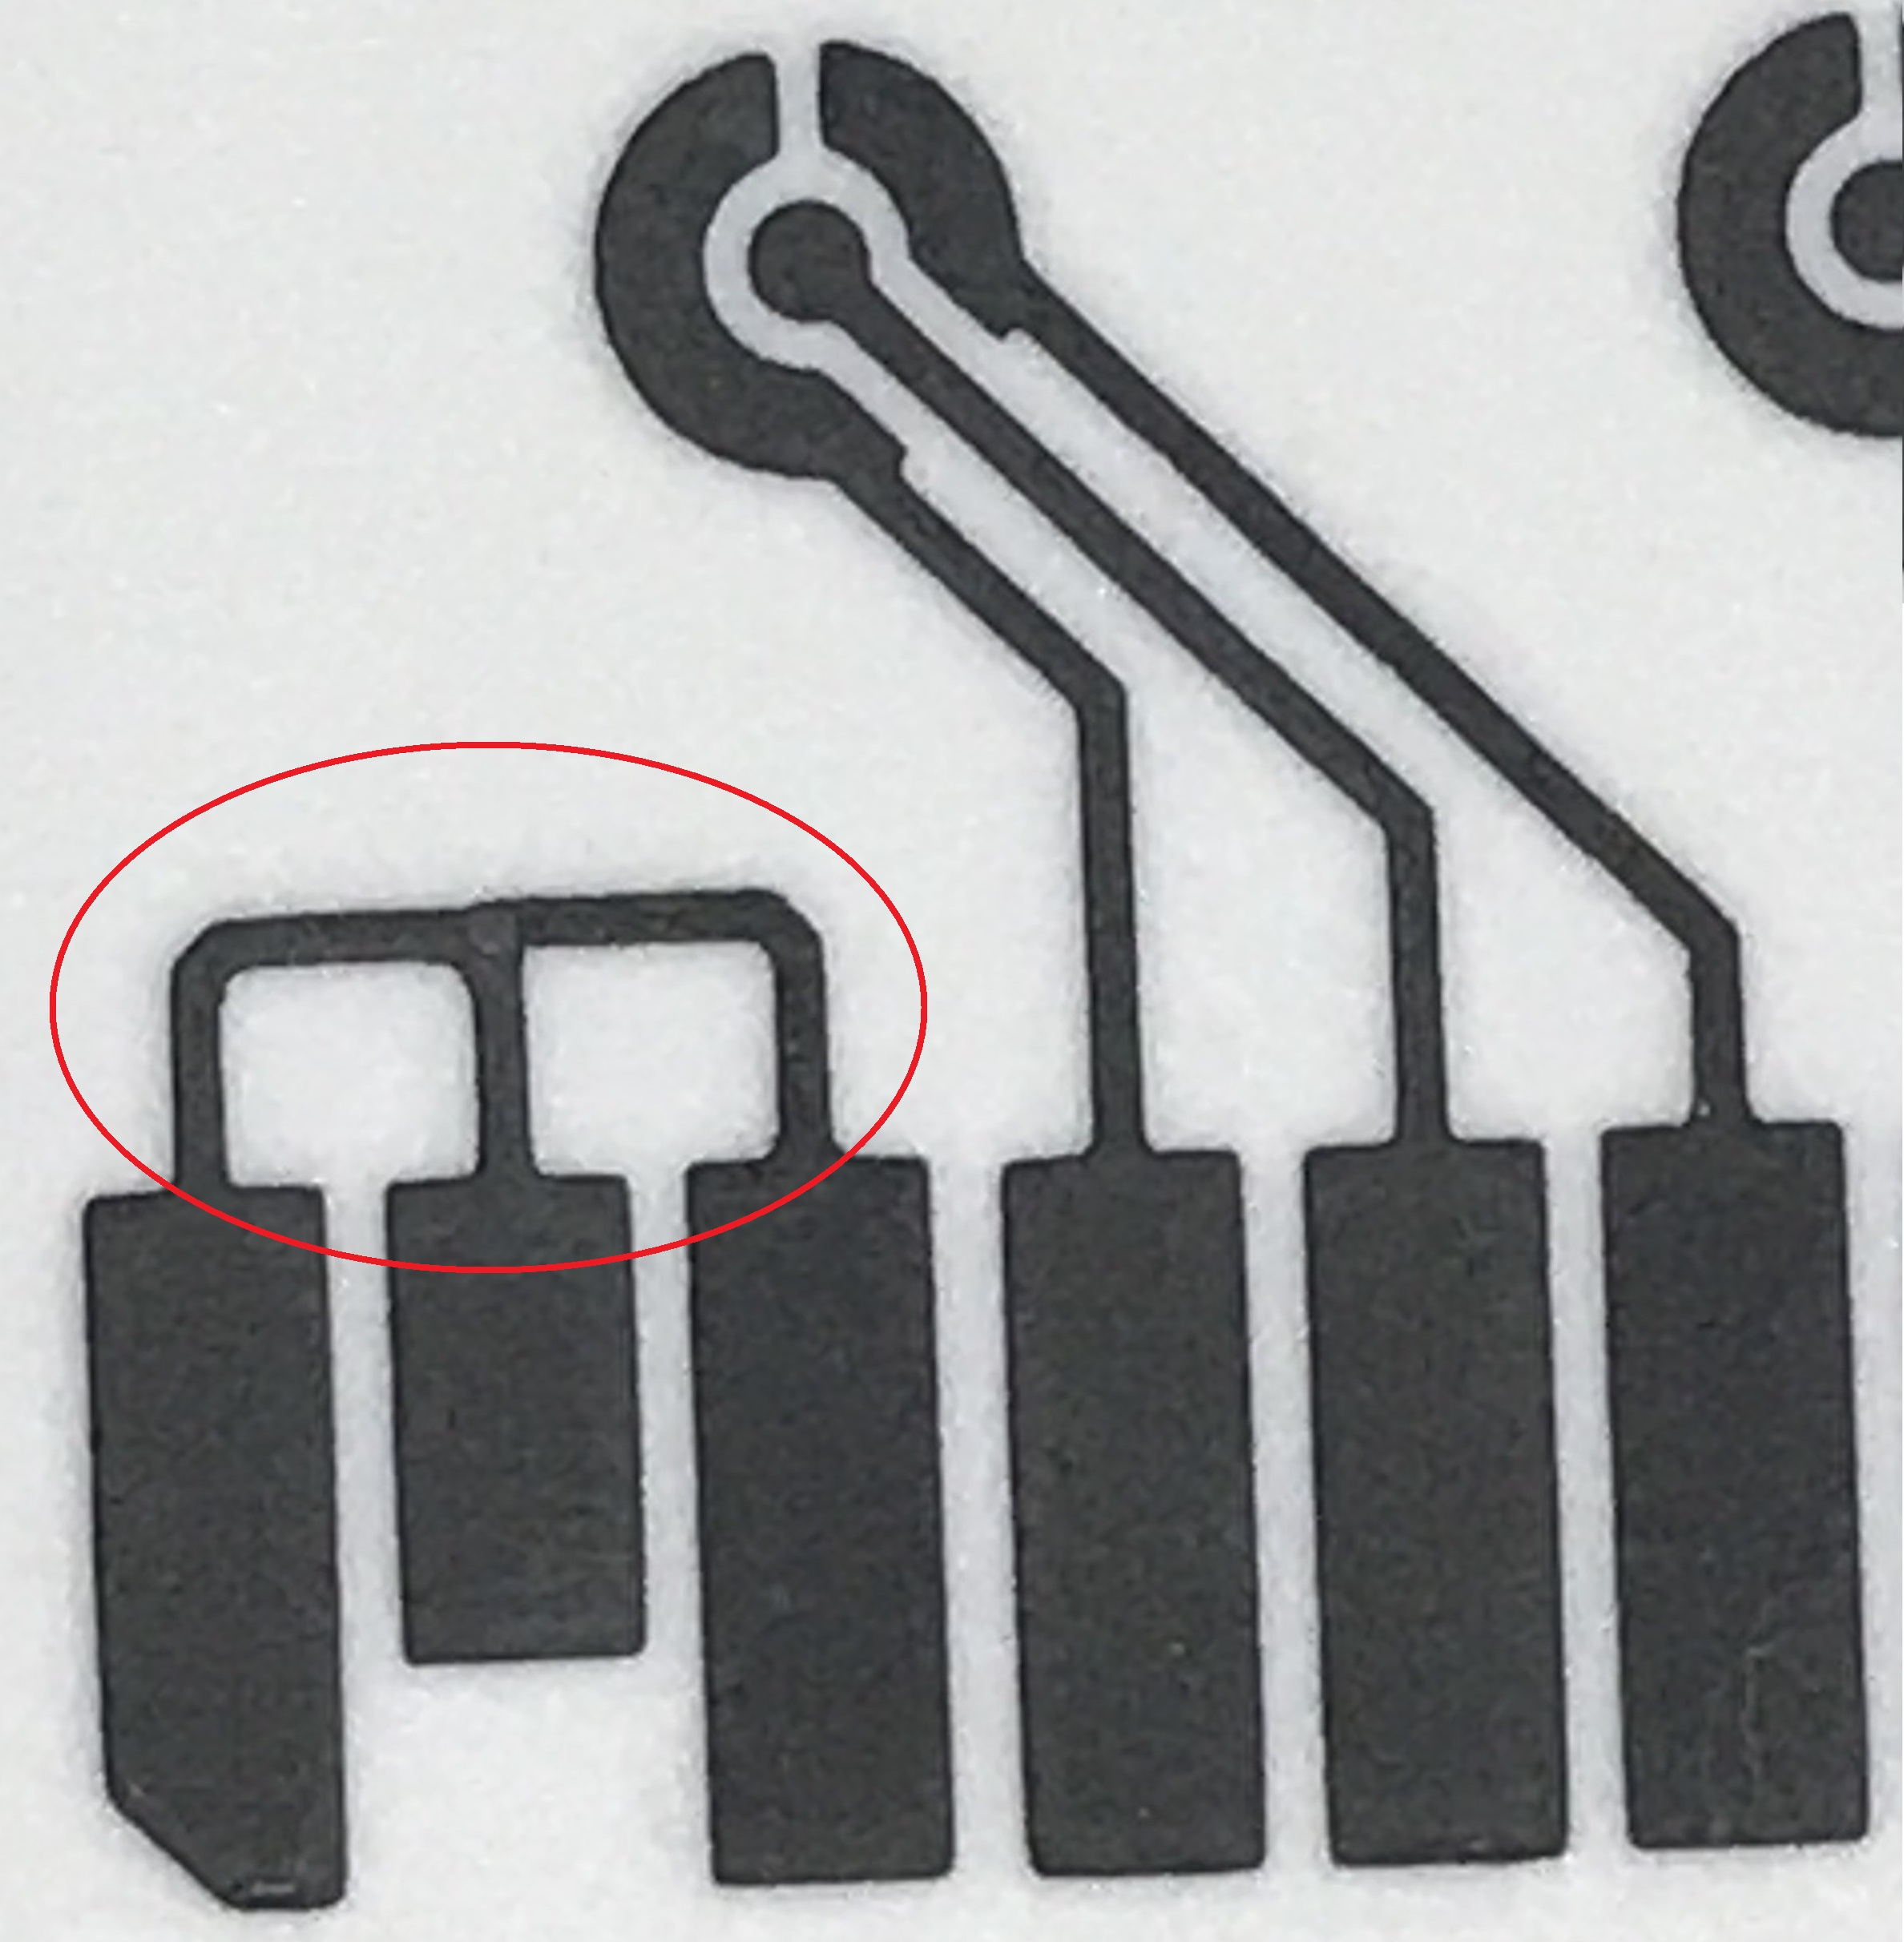
\includegraphics[width=0.45\textwidth]{Figures/Figura_contactos_prueba}
  \caption{Test contacts in biosensor.}
  \label{fig:Figura_contactos_prueba}
\end{figure}

The design is 2.5 mm high and 5.5 mm long, the path width is 0.4 mm. For this impression, no reference point was used, but the impression origin point was aligned with the beginning of the carbon pathways. An extra of 1 mm was added over the contacts for a better carbon-gold nanoparticle ratio. Given the good anchorage of the gold nanoparticle ink on the carbon, the desired design was obtained correctly, almost without spills (Figure ~\ref{fig:Figura_contactos_prueba_con_Oro}). Two layers of the design were printed, both cured on \textit{Hot Plate} at 80°C for 80 minutes.

\begin{figure}[H]
  \centering
    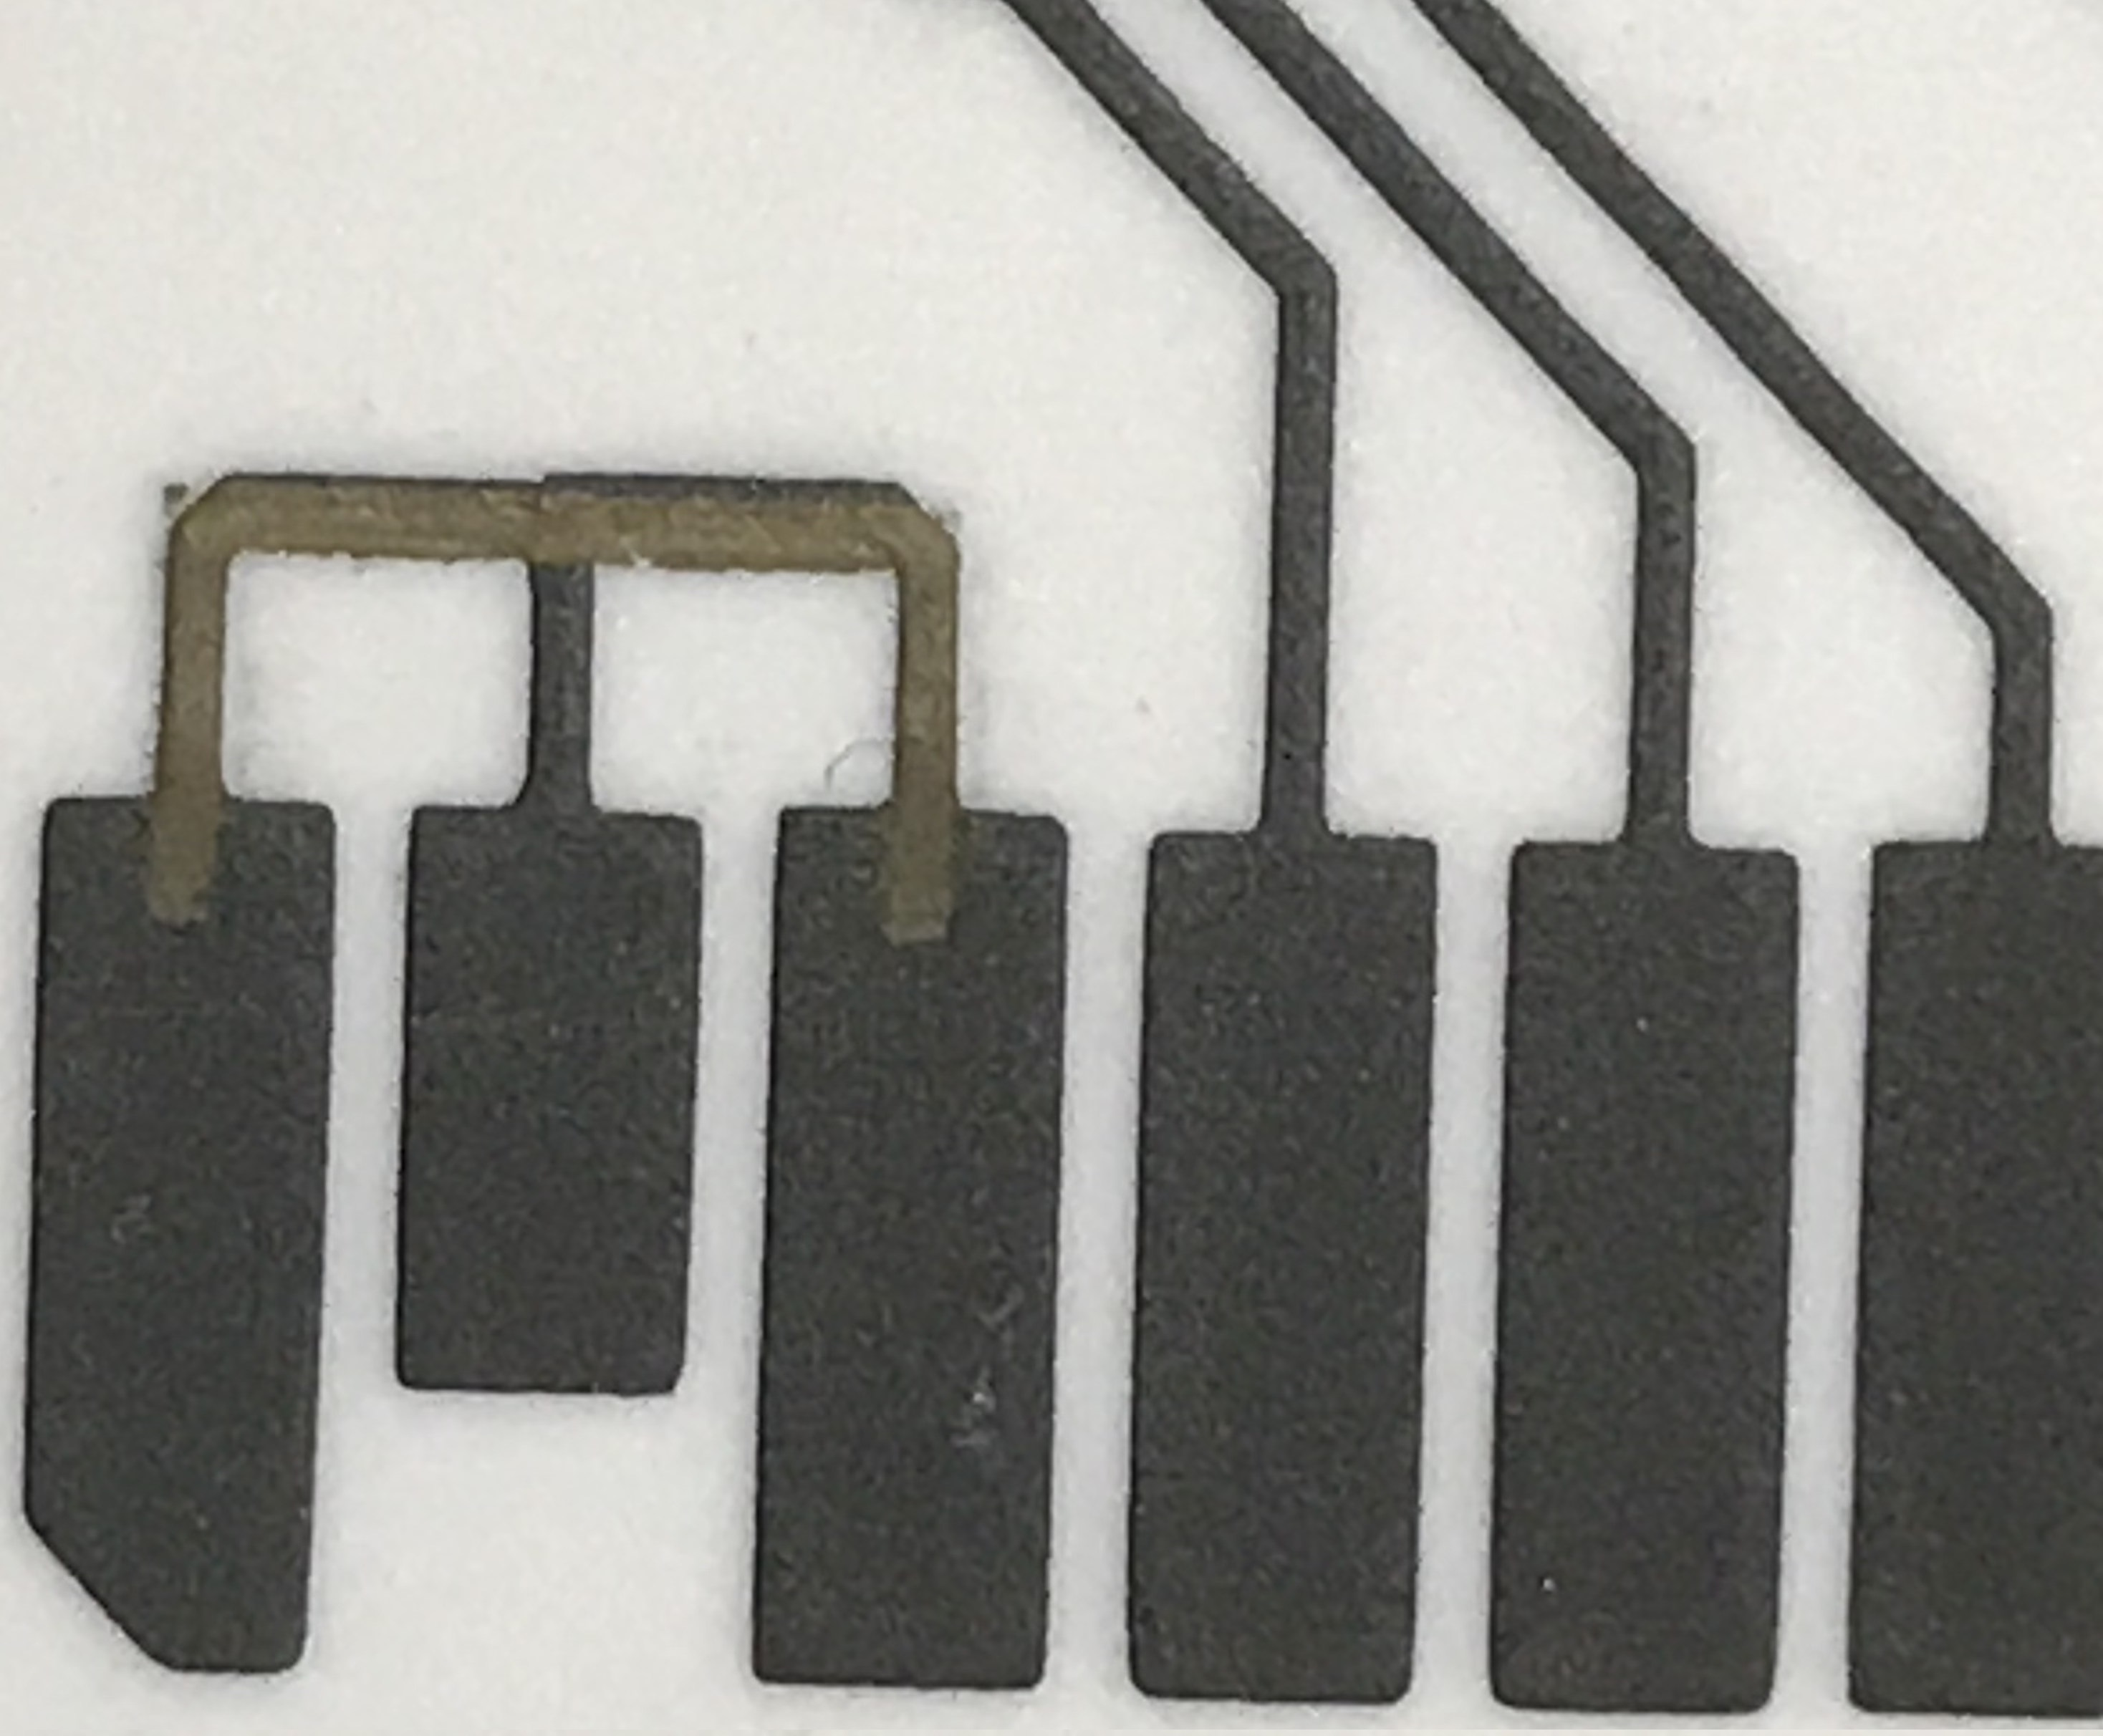
\includegraphics[width=0.45\textwidth]{Figures/Figura_contactos_prueba_con_Oro}
  \caption{Test contacts with printed gold nanoparticles ink.}
  \label{fig:Figura_contactos_prueba_con_Oro}
\end{figure}

In order to have a greater amount of tests in the electrochemical characterization, prints were made with gold nanoparticle ink on \textit{Valox} substrate, without carbon ink (Figure ~\ref{fig:Figura_impresion_sustrato_valox_tinta_Oro}), on a PET (Polyethylene Terephthalate) substrate and a cellulose pulp sheet (conventional notebook sheet).

\begin{figure}[H]
  \centering
    \includegraphics[width=0.5\textwidth]{Figures/Figura_impresion_sustrato_valox_tinta_Oro}
  \caption{Printing on \textit{Valox} substrate.}
  \label{fig:Figura_impresion_sustrato_valox_tinta_Oro}
\end{figure}

Two circles of 1 mm diameter separated 16 mm were printed on the \textit{Valox} substrate and the cellulose pulp sheet, which were then joined by a line 17 mm long and 0.4 mm wide, thus the ink was printed from half a circle to half the other, ensuring the continuity of the material. Two identical layers were printed, for the \textit{Valox} substrate a cure was made between each impression in \textit{Hot Plate} at 80ºC for 80 minutes.

A different design was made for the PET substrate (Figure ~\ref{fig:Figura_impresion_sobre_PET}) because there was no reference to how the ink would anchor on the base. An arrangement of six drawings was made in two columns, composed of two squares of 1 mm side separated 16 mm and a bar 17 mm long and 0.4 mm wide. The separation between columns is 65 mm and 20 mm between rows. The separation into columns is due to the fact that half of the substrate was cleaned with ethyl alcohol, in this way, will be observed the differences between the treated and untreated substrate. Two identical layers were printed with their respective cures on \textit{Hot Plate} at 80°C for 80 minutes.

\begin{figure}[H]
  \centering
    \includegraphics[width=0.5\textwidth]{Figures/Figura_impresion_sobre_PET}
  \caption{Printed design on PET substrate.}
  \label{fig:Figura_impresion_sobre_PET}
\end{figure}

\section{Characterizations}
\subsection{Electrical characterization}
The electrical characterization consists of the 4-tip resistance measurement, explained earlier in Chapter 2, \hyperref[subsec:carac_elec]{section 2.3.1}. The resistance measurements were made on carbon ink, carbon ink plus one layer, and two layers of cured gold nanoparticles ink.

It should be noted that the results obtained from this measurement is made up of an electrical parallel between the resistance of the carbon ink and the resistance of the gold nanoparticles ink. A considerable decrease in resistance was obtained (compared to a parallel of two carbon resistors) in accordance with the proposed theory, since the resistivity of gold (2.44·10\textsuperscript{-8} Ohm·m) is much lower than that of carbon (3.5·10\textsuperscript{-5} Ohm·m) \cite{Resistividad}.

\subsection{Dimensional characterization}
For the dimensional characterization the fiducial camera of the \textit{Dimatix} printer was used, obtaining the dimensions of the \emph{WE} and the separations between it, the \emph{CE} and the \emph{RE} (Figure ~\ref{fig:Figura_medicion_WE}).

\begin{figure}[H]
  \centering
    \includegraphics[width=0.5\textwidth]{Figures/Figura_medicion_WE}
  \caption{\emph{WE} diameter measurement.}
  \label{fig:Figura_medicion_WE}
\end{figure}

The roughness and thickness of the carbon film and the film obtained with the gold nanoparticles ink were obtained using a \textit{Bruker} model \textit{Dektak XT} contact profilometer with a 12.5 $\mu$m \textit{Stylus} tip (Figure ~\ref{fig:Figura_Perfilometro}). The force applied by the tip was in both cases 3 mgf.

\begin{figure}[H]
  \centering
    \includegraphics[width=0.5\textwidth]{Figures/Figura_Perfilometro}
  \caption{Dektak XT Advanced Profilometer.}
  \label{fig:Figura_Perfilometro}
\end{figure}

For this characterization, a 2000 $\mu$m path was determined on the working electrode for 15 seconds and then the area of interest was selected to measure the roughness. Three values were taken on the entire sample:

$\bullet$ The average value of maximum roughness (Rz).

$\bullet$ The highest peak roughness (Rt).

$\bullet$ The average roughness value (Ra).
\\

To characterize the thickness of the \emph{WE}, a path of 1000 $\mu$m was set for 15 seconds. The length of the route was determined at that value in order to obtain the rise/fall steps and with this obtain a reference (Figure ~\ref{fig:Figura_grafico_perfilometro}). To determine the thickness of the gold ink, the thickness of a carbon pad and that of a \emph{WE} with gold nanoparticles ink were measured. Making the difference between the two, the thickness of two layers of gold ink printed by \textit{Inkjet} was obtained.

\begin{figure}[H]
  \centering
    \includegraphics[width=0.8\textwidth]{Figures/Figura_grafico_perfilometro}
  \caption{Thickness characterization graph.}
  \label{fig:Figura_grafico_perfilometro}
\end{figure}

For these studies, two samples were used, identified as nPoc3 and nPoc5 cartridges, having two cured layers of 1 mm and 1.1 mm in diameter (Gold nanoparticles ink) respectively. From each one, the working electrodes identified as 3 and 4 were used to obtain a varied sampling. Two measurements were made on each and then averaged.

\subsection{Electrochemical characterization}
The electrochemical characterization was carried out on different configurations of substrates and inks to obtain multiple comparisons of interest for the project. Samples are listed in test order (Figure ~\ref{fig:Figura_pruebas_muestras}):

$\bullet$ Gold thin film electrode deposited by sputtering on silicon. (Figure ~\ref{fig:Figura_pruebas_muestras} (a))

$\bullet$ Screen printed carbon film electrode on \textit{Valox} substrate. (Figure ~\ref{fig:Figura_pruebas_muestras} (b))

$\bullet$ Screen printed carbon film electrode and inkjet printed gold nanoparticles ink of 1 mm diameter on \textit{Valox} substrate. (Figure ~\ref{fig:Figura_pruebas_muestras} (c))

$\bullet$ Screen printed carbon film electrode and inkjet printed gold nanoparticles ink of 1.1 mm diameter on \textit{Valox} substrate.

$\bullet$ Inkjet printed gold nanoparticles ink on \textit{Valox} substrate.

$\bullet$ Inkjet printed gold nanoparticles ink on PET substrate. (Figure ~\ref{fig:Figura_pruebas_muestras} (d))

$\bullet$ Inkjet printed gold nanoparticles ink on cellulose pulp substrate. (Figure ~\ref{fig:Figura_pruebas_muestras} (e))

\begin{figure}[H]
  \centering
    \includegraphics[width=1\textwidth]{Figures/Figura_pruebas_muestras}
  \caption{Samples where the electrochemical characterization was carried out.}
  \label{fig:Figura_pruebas_muestras}
\end{figure}
To make the tests comparable to each other, a 2 cm\textsuperscript{2} area platinum counter electrode and a \textit{Cole-Parmer} reference mercury(I) chloride or saturated \textit{Calomel} (Hg\textsubscript{2}Cl\textsubscript{2}) electrode were used, both external to the samples. The electrochemical cell reservoir was made of acrylic with an approximate volume of 3 ml. It has a hole at the bottom where polypropylene seals can be placed. In the experiments a 1 mm diameter seal was used, to have the same geometric area of 0.785 mm\textsuperscript{2} in all the tests.

After contacting the seal with the electrode, the cell is filled from the top with the ferrocyanide (K\textsubscript{4}Fe(CN)\textsubscript{6}) and ferricyanide (K\textsubscript{3}Fe(CN)\textsubscript{6}) probe solution and the supporting electrolyte of potassium chloride (KCl). It was verified that there were no leaks (Figure ~\ref{fig:Figura_prueba_electroquimica}).

\begin{figure}[H]
  \centering
    \includegraphics[width=0.5\textwidth]{Figures/Figura_prueba_electroquimica}
  \caption{Experimental setup for electrochemical measurements.}
  \label{fig:Figura_prueba_electroquimica}
\end{figure}

Special care must be taken so that the seal does not obstruct part of the working electrode, otherwise it will not be completely covered by the probe solution (Figure ~\ref{fig:Figura_electrodo_sonda}). In addition, it must be verified that when filling the cuvette no bubbles are formed, since the working electrode would not be completely covered either.

\begin{figure}[H]
  \centering
    \includegraphics[width=0.5\textwidth]{Figures/Figura_electrodo_sonda}
  \caption{View of the Electrode in the acrylic cell.}
  \label{fig:Figura_electrodo_sonda}
\end{figure}

Measurements were taken with a \textit{Teq4} potentiostat. The excitation signal is a linear potential sweep with a triangular waveform of minimum potential E1 (-200 mV) and a maximum potential E2 (500 mV), with a sweep speed of 50 mV·s\textsuperscript{-1}. Using the potentiostat software, voltages and currents data were taken and exported in \textit{comma separated values} (CSV) format to be further processed in open source software \textit{GNUplot}. In addition, the graphics made by the potentiostat software were saved in PNG format as reference (Figure ~\ref{fig:Figura_software_potenciostato}).

\begin{figure}[H]
  \centering
    \includegraphics[width=0.5\textwidth]{Figures/Figura_software_potenciostato}
  \caption{\textit{Teq4} potentiostat software with measurement graph.}
  \label{fig:Figura_software_potenciostato}
\end{figure}

Once the experiments were carried out on all the samples, the data was processed to know the results and conclusions of the project.

\section{Photo-definable dielectric ink}
\label{sec:tinta_dielec}
This section will set out a project to continue, as a next step to the printing of gold nanoparticles on the working electrodes. Using the photo-definable dielectric ink, micro cuvettes will be made around the \emph{WE}. To generate these 3D structures by \textit{Inkjet} printing, several layers must be printed with their respective cures, forming a cylinder centered on each of the eight \emph{WE}. In this way, it is sought to form a container for each electrochemical cell, where the samples to be analyzed will be deposited. The main advantage for which this project is proposed is to use the \textit{Inkjet} printer for the complete manufacture of the biosensor, without the need to use other processes.

\subsection{Design}
Taking the dimensions of the working electrodes, 3 rings of different sizes were designed as a first approximation. These figures, printed in several layers, will form the microcuvette that will keep the sample contained on the electrochemical cell. The dimensions of the designs were 1050, 1100 and 1150 $\mu$m internal radius and 1350, 1300 and 1250 $\mu$m external radius, respectively. (Figure ~\ref{fig:Figura_anillos_SU8}).

\begin{figure}[H]
  \centering
    \includegraphics[width=0.5\textwidth]{Figures/Figura_anillos_SU8}
  \caption{(a) Ring from 1050 to 1350 $\mu$m. (b) Ring from 1100 to 1300 $\mu$m. (c) Ring from 1150 to 1250 $\mu$m.}
  \label{fig:Figura_anillos_SU8}
\end{figure}

In this way rings of 100, 200 and 300 $\mu$m thick are obtained, with which the optimal values for the printing of several successive layers will be determined, forming the microcuvette.

\subsection{Ink cartridge preparation}
For the formulation of the ink, a resin called \textit{SU-8 2007} was used as the solute and Cyclohexanone as the solvent (Figure ~\ref{fig:Figura_SU8_Ciclohexanona}). To obtain the proper viscosity to form and eject the ink droplets, the necessary proportion of each compound was calculated. It was determined that 2 ml of Cyclohexanone is necessary for every 3 ml of \textit{SU-8 2007}.

\begin{figure}[H]
  \centering
    \includegraphics[width=0.5\textwidth]{Figures/Figura_SU8_Ciclohexanona}
  \caption{Solute and solvent to formulate the photo-definable dielectric ink.}
  \label{fig:Figura_SU8_Ciclohexanona}
\end{figure}

Since said solute is photosensitive, the preparation had to be done in a dark room with UV filters. The cartridge reservoir had to be protected from UV rays because the printer is not in a dark room with the appropriate filters, which would dry the ink inside the reservoir. For this, aluminum foil was used, forming a cover, without blocking the head and its connections with the reel (Figure ~\ref{fig:Figura_cartucho_SU8}).

\begin{figure}[H]
  \centering
    \includegraphics[width=0.5\textwidth]{Figures/Figura_cartucho_SU8}
  \caption{SU-8 ink cartridge protected from UV rays.}
  \label{fig:Figura_cartucho_SU8}
\end{figure}

\subsection{Printer setup and calibration}
When installing the ink cartridge in the printer, the parameters of the ink cartridge were configured using the information provided by the manufacturer \textit{Microchem} \cite{PriElexSU8}, and the first ink ejection tests were carried out on the \textit{Drop Watcher} (Figure ~\ref{fig:Figura_Drop_Watcher_SU8}).

\begin{figure}[H]
  \centering
    \includegraphics[width=0.5\textwidth]{Figures/Figura_Drop_Watcher_SU8}
  \caption{SU-8 drops seen from the \textit{Drop Watcher} camera.}
  \label{fig:Figura_Drop_Watcher_SU8}
\end{figure}

Several purge cycles were necessary to obtain droplet ejection. The voltages of the nozzles were calibrated to have the same flight time between the 3 ejectors to be used.

\subsection{Prints}
The $``$\textit{Line Pattern}$"$ file was printed in order to define the spacing between drops necessary to obtain a continuous line with \textit{SU-8} ink on \textit{Valox} substrate. The optimal \textit{Drop Spacing}was defined to be 15 $\mu$m (Figure ~\ref{fig:Figura_LinePattern_SU8}).

\begin{figure}[H]
  \centering
    \includegraphics[width=0.5\textwidth]{Figures/Figura_LinePattern_SU8}
  \caption{Enlarged image of $``$\textit{Line Pattern}$"$ print.}
  \label{fig:Figura_LinePattern_SU8}
\end{figure}

For this \emph{DS}, the files to be printed must have a resolution of 1693.33 dpi as previously seen in Chapter 3, \hyperref[sec:calib_impresora]{section 3.2}.

Once the imported files were configured using the \textit{DMP} software, the first ring of radii 1050 $\mu$m inside and 1350 $\mu$m outside was printed (Figure ~\ref{fig:Figura_Anillo105a135_SU8}).

\begin{figure}[H]
  \centering
    \includegraphics[width=0.5\textwidth]{Figures/Figura_Anillo105a135_SU8}
  \caption{Printing ring of radii 1050 $\mu$m inside and 1350 $\mu$m outside.}
  \label{fig:Figura_Anillo105a135_SU8}
\end{figure}

Subsequently, a ring with 1100 $\mu$m of internal and 1300 $\mu$m of external radio was printed (Figure ~\ref{fig:Figura_Anillo110a130_SU8}).

\begin{figure}[H]
  \centering
    \includegraphics[width=0.5\textwidth]{Figures/Figura_Anillo110a130_SU8}
  \caption{Print of a ring with 1100 $\mu$m interior and 1300 $\mu$m exterior radio.}
  \label{fig:Figura_Anillo110a130_SU8}
\end{figure}

Finally, the 1150 $\mu$m interio and 1250 $\mu$m exterior radius ring was printed (Figure ~\ref{fig:Figura_Anillo115a125_SU8}).

\begin{figure}[H]
  \centering
    \includegraphics[width=0.5\textwidth]{Figures/Figura_Anillo115a125_SU8}
  \caption{Print of a ring with 1150 $\mu$m interior and 1250 $\mu$m exterior radio.}
  \label{fig:Figura_Anillo115a125_SU8}
\end{figure}

\subsection{Characterizations}
All new micro-cuvette electrochemical cell configurations, obtained by \textit{inkjet} printing with \textit{ad hoc} inks, will be characterized in future work.
\chapter{Mediciones y Resultados}
This chapter will summarize the measurements made and the results obtained after the development of the biosensors. It will be divided into three procedures differentiated by the type of characterization: electrical, dimensional and electrochemical.

\section{Caracterización eléctrica}
Four-point resistance measurements were made obtaining the following results:

$\bullet$ Between two carbon pads: \textbf{2,2 k$\Omega$}.

$\bullet$ Same carbon pads with a layer of cured gold nanoparticles ink: \textbf{1,15 k$\Omega$}.

$\bullet$ Same carbon pads with two layers of cured gold nanoparticles ink: \textbf{500 $\Omega$}.

Given the deposition of the gold ink layer on the carbon, a parallel is formed between the two elements. Using the equation of resistors in parallel (\ref{ecuacion1}), the resistance of the one and two cured layers of gold nanoparticles can be calculated.

\begin{equation}\label{ecuacion1}
R_{1//2}=\frac{R_{1} \times R_{2}}{R_{1}+R_{2}}
\end{equation}

De esta forma se obtienen los siguientes valores:

$\bullet$ A layer of cured gold nanoparticles: \textbf{2,4 k$\Omega$}.

$\bullet$ Two layers of cured gold nanoparticles: \textbf{0,65 $\Omega$}.

Assuming that the gold layers are thin film prints, the equation (\ref{ecuacion2}) is used to obtain the resistivity of the material,

\begin{equation}\label{ecuacion2}
\rho_{Bulk}=\frac{R \times w \times t}{L}
\end{equation}

where $\rho$\textsubscript{Bulk} is the resistivity, $R$ the resistance, $w$ the width, $t$ the thickness and $L$ the length of the material. In this case, the gold nanoparticles path. The width of the design is 0.04 cm, the average thickness for two layers 0.00055 cm (obtained by profilometer) and the length 1.05 cm giving the following results:

$\bullet$ A layer of cured gold nanoparticles ink (assuming half the thickness): \textbf{0,025 $\Omega$ $\times$ cm}

$\bullet$ Two layers of cured gold nanoparticles ink: \textbf{0,0000136 $\Omega$ $\times$ cm o 13,6 $\mu\Omega$ $\times$ cm}

According to the materials resistivity table, pure gold has a resistivity of \textbf{2,35 $\mu\Omega$ $\times$ cm} \cite{Resistividad}.

\section{Dimensional characterization}
After optically measuring the eight electrodes in a cartridge, the diameter was averaged at \textbf{993 $\mu$m} and the separations between elements of the electrochemical cell at \textbf{390 $\mu$m}.

The table of the figure~\ref{fig:Figura_tabla_rugosidades} shows the results of the roughness obtained.

\begin{figure}[H]
  \centering
    \includegraphics[width=0.6\textwidth]{Figures/Figura_tabla_rugosidades}
  \caption{Roughness values obtained for two \emph{WE} from two biosensors (nPoc3 and nPoc5).}
  \label{fig:Figura_tabla_rugosidades}
\end{figure}

The thicknesses of the same \emph{WE} were measured on the same biosensors. In order to obtain the estimated thickness of the 2 layers printed with the gold nanoparticles ink, the thickness was measured on a pure carbon electrode.

The table of the figure~\ref{fig:Figura_tabla_espesores} shows the values obtained from the thicknesses.

\begin{figure}[H]
  \centering
    \includegraphics[width=0.6\textwidth]{Figures/Figura_tabla_espesores}
  \caption{Thickness values obtained for two \emph{WE} of two biosensors (nPoc3 and nPoc5).}
  \label{fig:Figura_tabla_espesores}
\end{figure}

The tables were extracted from the report made at the Center for Physics and Metrology of the National Institute of Industrial Technology \cite{caracdimen}.

\section{Caracterización electroquímica}
The first cyclic voltammetry was performed with a pure gold electrode deposited on silicon using a \textit{Sputtering} process. The response for the ferro and ferricyanide electrochemical probes on a \textit{sputtering} deposited gold electrode was obtained (Figure ~\ref{fig:Figura_EQ_Oro_Sputtering_1mm}), which will be used as a reference to compare with electrodes printed with gold nanoparticles ink using the \textit{Inkjet} printing process.

\begin{figure}[H]
  \centering
    \includegraphics[width=0.8\textwidth]{Figures/Figura_EQ_Oro_Sputtering_1mm}
  \caption{Cyclic voltammetry with gold electrode obtained by Sputtering.}
  \label{fig:Figura_EQ_Oro_Sputtering_1mm}
\end{figure}

As a second measurement, it was decided to observe the behavior of the electrochemical probes on a carbon electrode (Figure ~\ref{fig:Figura_EQ_Carbono}), thus having the two curves that would overlap when testing a carbon electrode covered by the ink of gold nanoparticles.

\begin{figure}[H]
  \centering
    \includegraphics[width=0.8\textwidth]{Figures/Figura_EQ_Carbono}
  \caption{Cyclic voltammetry with carbon electrode.}
  \label{fig:Figura_EQ_Carbono}
\end{figure}
The next electrochemical measurement was performed on a carbon electrode coated with two layers of gold nanoparticle ink with 1 mm (Figure ~\ref{fig:Figura_EQ_Oro_Inkjet_Ambos} (a)) and 1.1 mm (Figure ~\ref{fig:Figura_EQ_Oro_Inkjet_Ambos} (b)) in diameter.

Comparing the result of the cyclical voltammetric curve of the electrochemical cell with gold \emph{WE} deposited by \textit{Sputtering} with the \emph{WE} with gold nanoparticles ink (Figure ~\ref{fig:Figura_EQ_Sputt_2-Inkjet}), the similarity is observed maintaining the current peaks corresponding to the gold.

\begin{figure}[H]
  \centering
    \includegraphics[width=1\textwidth]{Figures/Figura_EQ_Oro_Inkjet_Ambos}
  \caption{Cyclic voltammetry with carbon \emph{WE} coated with gold nanoparticles ink of different diameters: (a) 1 mm; (b) 1.1 mm.}
  \label{fig:Figura_EQ_Oro_Inkjet_Ambos}
\end{figure}

\begin{figure}[H]
  \centering
    \includegraphics[width=0.8\textwidth]{Figures/Figura_EQ_Sputt_2-Inkjet}
  \caption{Comparison of cyclic voltammetries of electrochemical cells with gold \emph{WE} deposited by \textit{Sputtering} and with carbon \emph{WE} with gold nanoparticles ink.}
  \label{fig:Figura_EQ_Sputt_2-Inkjet}
\end{figure}

The increase of intensity in the electrodes with gold \textit{inkjet} printing is due to the presence of carbon underneath it, as can be verified by overlapping the previous curves with that of pure carbon (Figure ~\ref{fig:Figura_EQ_Oro_Inkjet_Ambos}) and also, the increase in the effective area of the \emph{WE} due to the difference in roughness between the gold deposited by \textit{sputtering}  and the ink of gold nanoparticles printed by \textit{inkjet}.

\begin{figure}[H]
  \centering
    \includegraphics[width=0.8\textwidth]{Figures/Figura_EQ_Sptt_AuInkjet_Carbono_Valox}
  \caption{Overlapping \emph{WE} with gold deposited by \textit{Sputtering}, carbon \emph{WE} and carbon \emph{WE} with gold nanoparticles ink.}
  \label{fig:Figura_EQ_Sptt_AuInkjet_Carbono_Valox}
\end{figure}

To have comparisons of the nanoparticles ink on different substrates, measurements of the \textit{Inkjet} printed ink were made on Valox, PET and cellulose pulp sheet (Figure ~\ref{fig:Figura_EQ_Inkjet_Valox_PET_Papel}).

\begin{figure}[H]
  \centering
    \includegraphics[width=1\textwidth]{Figures/Figura_EQ_Inkjet_Valox_PET_Papel}
  \caption{Results of cyclic voltammetry on \textit{inkjet} printing of ink with gold nanoparticles on: (a) Valox; (b) PET and (c) Paper.}
  \label{fig:Figura_EQ_Inkjet_Valox_PET_Papel}
\end{figure}

The comparable results obtained between the gold deposited by \textit{Sputtering} and the \textit{Inkjet} printing on smooth substrate (PET) stands out (Figure ~\ref{fig:Figura_EQ_Sputt_Inkjet_PET}).

\begin{figure}[H]
  \centering
    \includegraphics[width=0.8\textwidth]{Figures/Figura_EQ_Sputt_Inkjet_PET}
  \caption{Comparison of cyclic voltammetry on \emph{WE} of gold deposited by \textit{Sputtering} and \textit{inkjet} printing of ink with gold nanoparticles on PET.}
  \label{fig:Figura_EQ_Sputt_Inkjet_PET}
\end{figure}
\chapter{Conclusions}

\section{Conclusions of the carried out work}
$\bullet$ Throughout this project, concentration and effort were dedicated to the improvement of a \textbf{biosensor} printed in carbon by silk screen printing using gold nanoparticles ink printed by the \textit{Inkjet} method. In turn, it seeks to achieve scalable manufacturing so that, if it is feasible, it can industrialize manufacturing.

$\bullet$ It is concluded that the gold nanoparticles ink has an acceptable anchorage with carbon ink, achieving the designs with acceptable precision. However, on a rough substrate (\textit{Valox}) does not achieve sufficient anchorage to be able to maintain the desired design.

$\bullet$ For a correct curing of each ink layer, it must be in \textit{Hot Plate} for at least 80 minutes at 80ºC.

$\bullet$ Two layers of ink with gold nanoparticles printed by \textit{Inkjet} have a thickness 3 times less than that of a carbon layer printed by screen printing.

$\bullet$ The resistivity of two cured layers is approximately 5 times greater than that of pure gold.

$\bullet$ The electrochemical capacity of a carbon \emph{WE} with 2 layers of cured gold nanoparticles is comparable to that of a gold \emph{WE} deposited by \textit{Sputtering}. Recalling the Randles-Sevcik equation \ref{ecuacion3}, the difference can be attributed, in part, to the difference in the effective areas of the \emph{WE}. Although geometrically identical (1 mm in diameter), the roughness generates a difference in the effective value used in the calculations. The advantages of \textit{inkjet} printing are ease of manufacture and considerably lower cost.

$\bullet$ The printing of two layers of gold nanoparticles ink by \textit{Inkjet} on a smooth substrate at the macroscopic level such as PET, approaches the cyclical voltammetry curve of the gold deposited by \textit{sputtering} on silicon, a smooth surface at the nanometric level.

$\bullet$ Correct droplet ejection and definition of droplet spacing were achieved for SU-8 dielectric ink. This allowed to make the prints with the desired design and motivated to continue with the development of this ink for future projects.

\section{Future work}
The present project on biosensors printed by \textit{Inkjet} method promotes, at least, two immediate steps to develop. The first linked to the composition and printing of carbon ink, to become independent of the intermediate step of screen printing. The second, and with greater impact, achieve the composition of a dielectric ink and its printing by \textit{Inkjet} method for the formation of microcuvettes that will contain the sample to be analyzed on the electrode, without having to go through other manufacturing processes.

In the Experimental Development section (Capítulo 3, \hyperref[sec:tinta_dielec]{section 3.5}) the formulation of the dielectric ink and the first test impressions with it are mentioned, which should be taken into account for the continuity of the technology development and the next improvements in the biosensors.

\nocite{Banica}
\nocite{Prudenziati}
\nocite{Voros}
\nocite{Poc}
\nocite{PosterPoc1}
\nocite{DMPDatasheet}
\nocite{AgParticlesDimatix1}
\nocite{AgParticlesDimatix2}

%% # Apendices de la tesis #
\appendix
\renewcommand{\appendixname}{Anexo}
\chapter{Configuración de impresora}\label{chap:apendiceA}
To start the print job, the procedure manual included with the device \cite{DimatixUM} should be readed and understood. In turn, given the high complexity of these works, publications made at the University of Pennsylvania \cite{UPenn} and the University of Michigan \cite{UMic} were analyzed, where calibrations and sample handling are explained in more detail.

The printer (Figure ~\ref{fig:Figura_Impresora_DMP2850}) consists of a platen with a vacuum system to hold samples and a heating system.

\begin{figure}[H]
  \centering
    \includegraphics[width=0.5\textwidth]{Figures/Figura_Impresora_DMP2850}
  \caption{Fujifilm Dimatix DMP-2850 printer.}
  \label{fig:Figura_Impresora_DMP2850}
\end{figure}

The print head carrying base has a system to vary the angle of the ink cartridge and thus modify the distance between drops of the different ejectors (Figure ~\ref{fig:Figura_Carriage_angulo}) and a fiducial camera, which allows viewing the substrate and printing in real time and making measurements through the Software included with the printer (Figure ~\ref{fig:Figura_Vista_Camara_Fiducial}). 

\begin{figure}[H]
  \centering
    \includegraphics[width=0.8\textwidth]{Figures/Figura_Carriage_angulo}
  \caption{a) Print head carrying system b) System to modify the angle of the cartridge.}
  \label{fig:Figura_Carriage_angulo}
\end{figure}

\begin{figure}[H]
  \centering
    \includegraphics[width=0.5\textwidth]{Figures/Figura_Vista_Camara_Fiducial}
  \caption{Fiducial camera view from DMP Software.}
  \label{fig:Figura_Vista_Camara_Fiducial}
\end{figure}

To observe the status of the head, the ejection of the drops and to calibrate the printing system, the \textit{Drop Watcher} is used. This system consists of a camera oriented at 45º from the horizontal plane, with focus on the ejectors of the head (Figure ~\ref{fig:Figura_Drop_Watcher}). Using a strobe light, photographs or filming of the operation of each of the head holes can be taken (Figure ~\ref{fig:Figura_Drop_Watcher}).

\begin{figure}[H]
  \centering
    \includegraphics[width=0.5\textwidth]{Figures/Figura_Camara_Drop_Watcher}
  \caption{\textit{Drop Watcher} camera, light and reservoir system.}
  \label{fig:Figura_Camara_Drop_Watcher}
\end{figure}

\begin{figure}[H]
  \centering
    \includegraphics[width=0.5\textwidth]{Figures/Figura_Drop_Watcher}
  \caption{Image of drops being ejected using DMP Software.}
  \label{fig:Figura_Drop_Watcher}
\end{figure}

\section{Ink cartridge preparation}
Since the reservoirs and heads can only be used with one type of ink, Fujifilm offers them in the form of Printing Kits (Figure ~\ref{fig:Figura_kit_impresion}). Each Kit consists of a 3 ml reservoir, a head (depending on the model it can be 1 pl or 10 pl, referring to the volume of the drop ejected), a 3 ml syringe, a round tip needle and a $``$\textit{cleaning pad}$"$ Figure ~\ref{fig:Figura_Cleaning_pad}). The size of the syringe does not allow a larger volume of ink to be deposited than that supported by the reservoir system. The length of the needle prevents breakage of the cartridge container.

\begin{figure}[H]
  \centering
    \includegraphics[width=0.5\textwidth]{Figures/Figura_kit_impresion}
  \caption{Print kit for Fujifilm Dimatix DMP2850 with 10 pl printhead filled with gold nanoparticles ink.}
  \label{fig:Figura_kit_impresion}
\end{figure}

\begin{figure}[H]
  \centering
    \includegraphics[width=0.5\textwidth]{Figures/Figura_Cleaning_pad}
  \caption{Usage of \textit{Cleaning Pad}.}
  \label{fig:Figura_Cleaning_pad}
\end{figure}

The \textit{Cleaning Pad} should be replaced once it is saturated with ink. This will be noticed by an excess of material on the substrate, the clogging of the ejectors or irregularities in the printing, such as misalignment of the drops on the substrate. To check if it is ink deposited on the head, the \textit{Drop Watcher} is used, where you can easily see the state of the ejectors and the flight of the drops (Figure ~\ref{fig:Figura_suciedad_cabezal}).

\begin{figure}[H]
  \centering
    \includegraphics[width=0.5\textwidth]{Figures/Figura_suciedad_cabezal}
  \caption{Ink deposited on the head due to the saturated \textit{Cleaning Pad}.}
  \label{fig:Figura_suciedad_cabezal}
\end{figure}

In the first instance, the quantity of ink to be used with the syringe is taken and deposited inside the reservoir. The length of the needle does not allow reaching the end of the reservoir, preventing perforation (Figure ~\ref{fig:Figura_carga_tinta}).

\begin{figure}[H]
  \centering
    \includegraphics[width=1\textwidth]{Figures/Figura_carga_tinta}
  \caption{Reservoir filling procedure.}
  \label{fig:Figura_carga_tinta}
\end{figure}

Once the reservoir is filled with the desired ink, the reservoir is installed over the head. Since it has a connection to a pressure line to generate a vacuum inside by helping the ink movement, the cartridge can only be assembled in one direction. According to Fujifilm's recommendations, it should be adjusted first on the side of the vacuum connector, pressing until you hear a $``$\textit{click}$"$, then check that the ink tank is aligned with the head and force it again until you hear a second $``$\textit{click}$"$. In this way, the ink tank is anchored to the head.

The cartridge must be inserted into the reel (Figure ~\ref{fig:Figura_Carrete1}) keeping in mind that the correct orientation is that which allows the head contacts to be aligned with those of the reel. For this the printer must be turned on and the \textit{Dimatix Drop Manager} Software running with its complete initial checkup procedure.

\begin{figure}[H]
  \centering
    \includegraphics[width=0.5\textwidth]{Figures/Figura_Carrete1}
  \caption{Reel with the cartridge is installed.}
  \label{fig:Figura_Carrete1}
\end{figure}

Once the cartridge is installed, the \textit{Cleaning Pad} is placed in the dedicated hole for this object (Figure ~\ref{fig:Figura_Orificio_Cleaning_Pad}). This should be done before closing the cartridge installation procedure to avoid spilling ink on the reel rest base.

\begin{figure}[H]
  \centering
    \includegraphics[width=0.5\textwidth]{Figures/Figura_Orificio_Cleaning_Pad}
  \caption{\textit{Cleaning Pad} location.}
  \label{fig:Figura_Orificio_Cleaning_Pad}
\end{figure}

By closing the printer cover, the cartridge installation procedure is completed and the software asks to load the configuration file, which is unique for each ink. Within this file is the waveform that handles the ejectors (Figure ~\ref{fig:Figura_Pantalla_Waveform}) and the parameters adjusted so that the formation and deposition of the drops of the material is possible. Within these parameters are the upper limit of voltage for each ejector, the temperature of the head, the vacuum pressure to generate the ink meniscus, the height at which the cartridge will move with respect to the substrate and the cleaning cycles before, during and after printing (Figure ~\ref{fig:Figura_Configuraciones_cartucho}).

\begin{figure}[H]
  \centering
    \includegraphics[width=0.5\textwidth]{Figures/Figura_Pantalla_Waveform}
  \caption{Setup screen with Waveform.}
  \label{fig:Figura_Pantalla_Waveform}
\end{figure}

\begin{figure}[H]
  \centering
    \includegraphics[width=0.8\textwidth]{Figures/Figura_Configuraciones_cartucho}
  \caption{Screens for setting of the printing parameters.}
  \label{fig:Figura_Configuraciones_cartucho}
\end{figure}

To check the correct operation of the system, the \textit{Drop Watcher} is used where the ejection of the drops from the configured \textit{nozzles} can be seen in real time and, at the same time, the voltage adjustment can be made to match the flight time of the different ejectors (Figure ~\ref{fig:Figura_drop_watcher1}).

\begin{figure}[H]
  \centering
    \includegraphics[width=0.5\textwidth]{Figures/Figura_drop_watcher1}
  \caption{Drop Watcher screen.}
  \label{fig:Figura_drop_watcher1}
\end{figure}

Once the use of the cartridge is finished, it must be placed vertically, otherwise the channel that feeds the head will empty of ink (Figure ~\ref{fig:Figura_canal_cartucho_vacio}). If this happens, several purge cycles must be carried out or fill with more ink, but there is no guarantee that the cartridge will work properly again.

\begin{figure}[H]
  \centering
    \includegraphics[width=1\textwidth]{Figures/Figura_canal_cartucho_vacio}
  \caption{Cartridge channel without ink.}
  \label{fig:Figura_canal_cartucho_vacio}
\end{figure}

\section{Substrate clamping and platen configuration}
The printer platen is a metal surface with an arrangement of holes where a vacuum is generated to suck the substrate on which is wanted to print (Figure ~\ref{fig:Figura_platina}). Although the vacuum generated in the holes is considerable, special attention must be paid to ensure that the entire surface is in contact, otherwise the clamping will not be sufficient to keep the substrate fixed at the time of printing. If all the holes are not obstructed by the substrate, the system will not generate the negative pressure stipulated by the manufacturer and the fixing will not be assured.

\begin{figure}[H]
  \centering
    \includegraphics[width=0.5\textwidth]{Figures/Figura_platina}
  \caption{Fujifilm Dimatix DMP-2850 Printer platen.}
  \label{fig:Figura_platina}
\end{figure}

To prevent these problems and ensure the correct anchorage of the surface to be printed, adhesive paper tape is used.

It is important that the base to be printed does not move during the entire printing process, paying the greatest attention after performing the \textit{Theta} calibration, explained in the section on Commissioning and calibration of the printer, since it compensates the angular \textit{offset} that can be generated between the substrate once fixed and the platen.

Once the substrate has been positioned and anchored, the thickness of the substrate and the temperature of the platen must be configured using the printer software. If adhesive tape was used to place the sample, it is advisable to add a greater thickness to avoid spool rubbing, ink loss, or head breakage.
\chapter{Project closure process}
\label{chap:apendiceB}

\section{Learned lessons}
In a research project it is vital to take note of all the work carried out and the results obtained. Having tracking codes of the different deliverables simplifies the development and knowledge of the history of each one.

Keeping the project monitoring files updated day by day helps to improve the quantity and quality of the information that is released.

Regarding to the project carried out, the following points are listed to be taken into account for future work:

$\bullet$ Before starting the printer, check that the printing area is free of obstacles.

$\bullet$ Keep the cartridges upright, with the head down, to prevent air from entering the reservoir channel.

$\bullet$ If the substrate is attached to the platen with adhesive tape, the thickness of it must be taken into account to add in the printing configurations.

$\bullet$ Before printing, check that the ejectors are working correctly and the ink drops have an aligned flight.

$\bullet$ Control the condition of the cleaning pad periodically, if the head begins to show ink drops on its base, it may be due to saturation of the drying material.

%% # Bibliografia #
\bibliography{bibliografia}

\end{document}